
\documentclass{workpackage}


\usepackage{ragged2e}
\usepackage{listings}
\usepackage{color}
\usepackage{url}
\usepackage{graphicx}
\usepackage{textcomp} % additional fonts, required for upquote in listings and \textmu
\usepackage{placeins} % FloatBarrier
\usepackage{url} % for websites
\usepackage[detect-weight]{siunitx} % nice! SI units and print numbers
\usepackage{afterpage} % afterpage{\clearpage}
\usepackage{gensymb} % get the degree symbol as in \celcius
\usepackage{amsmath} 
\usepackage[printonlyused]{acronym}
\usepackage{lastpage}

\usepackage{hyperref}

%the following is required for carriage return symbol
%ftp://ftp.botik.ru/rented/znamensk/CTAN/fonts/mathabx/texinputs/mathabx.dcl
%https://secure.kitserve.org.uk/content/mathabx-font-symbol-redefinition-clash-latex
\DeclareFontFamily{U}{mathb}{\hyphenchar\font45}
\DeclareFontShape{U}{mathb}{m}{n}{
      <5> <6> <7> <8> <9> <10> gen * mathb
      <10.95> mathb10 <12> <14.4> <17.28> <20.74> <24.88> mathb12
      }{}
\DeclareSymbolFont{mathb}{U}{mathb}{m}{n}
\DeclareMathSymbol{\dlsh}{3}{mathb}{"EA}

\usepackage[T1]{fontenc}

%enable smart resizing: large images are resized down but small images are left as they are
\usepackage[Export]{adjustbox}
\adjustboxset{max size={\textwidth}{0.7\textheight}}


\definecolor{LightGrey}{rgb}{0.95,0.95,0.95}
\definecolor{LightRed}{rgb}{1.0,0.9,0.9}

\lstset{ %
upquote=true, % gives the upquote instead of the curly quote
basicstyle=\ttfamily\tiny,       % the size of the fonts that are used for the code
numbers=none,                   % where to put the line-numbers
showspaces=false,               % show spaces adding particular underscores
showstringspaces=false,         % underline spaces within strings
showtabs=false,                 % show tabs within strings adding particular underscores
frame=lines,                   % adds a frame around the code
tabsize=4,              % sets default tabsize to 2 spaces
captionpos=b,                   % sets the caption-position to bottom
framesep=1pt,
xleftmargin=0pt,
xrightmargin=0pt,
 captionpos=t,                    % sets the caption-position to top
%deletekeywords={...},            % if you want to delete keywords from the given language
%escapeinside={\%*}{*)},          % if you want to add LaTeX within your code
%escapeinside={\%}{)},          % if you want to add a comment within your code
breaklines=true,        % sets automatic line breaking
breakatwhitespace=false,    % sets if automatic breaks should only happen at whitespace
prebreak=\raisebox{0ex}[0ex][0ex]{$\dlsh$} % add linebreak symbol
}

\lstdefinestyle{incellstyle}{
  backgroundcolor=\color{LightGrey},  % choose the background color,  add \usepackage{color}
  language=Python,
}

\lstdefinestyle{outcellstyle}{
  backgroundcolor=\color{LightRed},   % choose the background color; you must add \usepackage{color} or \usepackage{xcolor}
}

\usepackage[a4paper, margin=0.75in]{geometry}
\newlength{\textwidthm}
\setlength{\textwidthm}{\textwidth}

\newcommand\purl[1]{\protect\url{#1}} % "protected url"




% then follows the rest of the preamble to be placed before the begin document
% this preamble content is special to the documentclass you defined above.


\WPsubject{Standard Atmospheres}
\WPclassification{Unclassified}
\WPcurrentpackdate{\today}
\WPdocauthor{CJ Willers}
\newlength{\savedparskip}
\WPconclusions{
\setlength{\savedparskip}{\parskip}
\setlength{\parskip}{0.ex plus 0.1ex minus 0.3ex}
\begin{enumerate}
\item 
This work package describes several standard atmospheres used in previous projects: (1) Set-A, (2) OSSIM, and (3) Morticia.  The conditions cover typical and extreme conditions as used in the projects.
\item 
The atmospheric profiles captured here are not all equally analysed. Set-A is analysed in detail (most of this document describes various aspect of Set-A models. The OSSIM and Mortica atmospheric profiles are contained in the repository, but not analysed here.
\end{enumerate}
\setlength{\parskip}{\savedparskip}
}


%and finally the document begin.
\begin{document}
\WPlayout
\tableofcontents

\chapter{Introduction}

A number of 'standard' atmospheres were defined to cover the expected range of climatic conditions to be used in design analyses and optimisations.  This document defines and analyses the Modtran-calculated transmittance data.  Modtran 5.0 was used in these calculations.

The path definitions and data are stored in the git repository at\\
\verb+https://github.com/NelisW/StandardAtmospheres.git+


\section{Atmosphere Scenarios}
\label{sec:AtmosphereScenarios}


\subsection{OSSIM Atmosphere Scenarios}
\label{sec:OSSIMAtmosphereScenarios}

The OSSIM data files have two variations: a Lowtran version and a Modtran version. The Modtran version has the word Modtran appended to the filename.  The filenames have the \lstinline{*.inp} extension, but these are standard \lstinline{tape5} files.

OSSIM Modtran files are normally slant paths.

Modtran  lattitude/longitude conventions is North of the Equator and West of Greenwich.

The files reported here have aerosol types, surface albedo, visibility and date and time of day. OSSIM overwrites these values with the values supplied in the scenario files.

\subsubsection{DCOTBMLSNavMar15Nov11hMod4}
\label{sec:DCOTBMLSNavMar15Nov11hMod4}

\textbf{MLS, Navy Maritime, good 65~\si{\kilo\metre} visibility}

Mid-Latitude Summer, Navy Maritime aerosol with 4.1 \si{\metre\per\second} wind speed (current and 24-hour average) with visibility of 65~\si{\kilo\metre},
ground level P=1012~mbar, T=21C, RH=76\%, 14~g/m$^3$ absolute humidity.
The lattitude/longitude are -34.454\si{\degree} (South) and 339.601\si{\degree} (West from Greenwich).
Local time is 11:00 (09:00 GMT) on day 319 (15 November).

\subsubsection{Irene\purl{_}somer\purl{_}dag}
\label{sec:Irenesomerdag}

\textbf{Summer day in Pretoria, 23~\si{\kilo\metre} visibility}

Summer day in Irene, Pretoria.
User model (21 layers), 23~\si{\kilo\metre} visibility Rural aerosol,  ground level 1413~\si{metre} above sea level,  P=849~mbar, T=24.8C, RH=61\%, 13.9~g/m$^3$  absolute humidity.

\subsubsection{MidlatitudeSummer}
\label{sec:MidlatitudeSummer}

\textbf{MLS, moderate temperature, 23~\si{\kilo\metre} visibility}

MLS, 23~\si{\kilo\metre} visibility Rural aerosol,  P=1012~mbar, T=21C, RH=76\%, 14~g/m$^3$ absolute humidity.

\subsubsection{MidlatitudeWinter}
\label{sec:MidlatitudeWinter}

\textbf{MLW, cold,  23~\si{\kilo\metre} visibility}

MLW, 23~\si{\kilo\metre} visibility Rural aerosol,
  P=1018~mbar, T=-1C, RH=77\%, 3~g/m$^3$ absolute humidity.

\subsubsection{USStandardModtran}
\label{sec:USStandardModtran}

\textbf{US Standard, cool 23~\si{\kilo\metre} visibility}

US Standard, 23~\si{\kilo\metre} visibility Rural aerosol,
P=1013~mbar, T=15C, RH=46\%, 5.9~g/m$^3$ absolute humidity. 

\subsubsection{UserDefinedTemplate}
\label{sec:UserDefinedTemplate}

This file is not used directly in its original form in OSSIM. This file is a template used when a meteorological file is used. The meteorological file contents is used to overwrite some fields in this template file.

\subsubsection{Tropical}
\label{sec:Tropical}

\textbf{Moderate temperature, 23 km Rural visibility}

Tropical, 23 km visibility  Rural aerosol, ground level P=1013~mbar, T=26.5C, RH=75\%, 18.8~g/m$^3$ absolute humidity.

This is the same as Set-A TropicalUrban.

\subsubsection{SubarticWinter}
\label{sec:SubarticWinter}

\textbf{Sub-Artic winter day, very cold with moderate visibility}

Sub-Arctic Winter, 23 km visibility  Rural aerosol
 P=1013~mbar, T=-15.9C, RH=80\%, 1~g/m$^3$ absolute humidity.

\subsubsection{SubarticSummer:}
\label{sec:SubarticSummer}

\textbf{Scandinavian summer day }

Sub-Arctic Summer, 23 km visibility  Rural  aerosol, P=1010~mbar, T=14C, RH=75\%, 9~g/m$^3$ absolute humidity.


\subsubsection{PretoriaTropicalRural23km15NovXXh}
\label{sec:PretoriaTropicalRural23km15NovXXh}

\textbf{Warm temperature, 23 km Rural visibility, different times of day}

Tropical, 23 km visibility  Rural aerosol, ground level P=1013~mbar, T=26.5C, RH=75\%, 18.8~g/m$^3$ absolute humidity.
The lattitude/longitude are for Pretoria at  -25.75\si{\degree} (South) and 331.71\si{\degree} (West from Greenwich).
Three different local times are used in the separate files [09:00, 12:00, 15:00] (07:00, 10:00, 13:00 GMT) on day 319 (15 November).

The terrain albedo is zero for all the terrains, except for 
\lstinline{PretoriaTropicalRural23km15Nov09h-desertAlbedo} which uses the Modtran desert albedo.


\subsubsection{Overberg\purl{_}2\purl{_}2\purl{_}1996}
\label{sec:Overberg221996}

\textbf{Summer day in Pretoria, 23~\si{\kilo\metre} visibility}

Summer day at Overberg Test Range, Western Cape.
User model (33 layers), 23~\si{\kilo\metre} visibility Rural aerosol,  0~\si{metre} above sea level,   at ground level P=1011~mbar, T=26.5C, RH=69\%, 17.3~g/m$^3$  absolute humidity.



\subsection{Morticia Atmosphere Scenarios}
\label{sec:MorticiaAtmosphereScenarios}

To be completed later.

\subsection{Set-A Atmosphere Scenarios}
\label{sec:SetAAtmosphereScenarios}


\subsubsection{ExtremeHotLowHumidity}
\label{sec:ExtremeHotLowHumidity}

\textbf{very hot, low humidity, 75 km Desert visibility - no wind, clear day in the desert}

User model (36 layers), 70 km visibility  Desert aerosol, ground level P=1030~mbar, T=44C, RH=30\%, 18.1~g/m$^3$  absolute humidity.

\subsubsection{ExtremeHumidity:}
\label{sec:ExtremeHumidity}

\textbf{very high humidity - Arabian gulf, tropical Africa / Amazon}

User model (36 layers), 23 km visibility  Rural aerosol, ground level P=1030~mbar, T=35C, RH=95\%, 37.9~g/m$^3$ absolute humidity. 
At sea level, this atmosphere corresponds with  the highest recorded dew point at 34~$^\circ$C.  MIL-HDBK-310 indicates that the probability of absolute humidity exceeding this level is significantly less than 1\%. This corresponds to the highest recorded humidity ever, recorded in Sharjah in the UAE.

\subsubsection{MidLatMaritimeSummer:}
\label{sec:MidLatMaritimeSummer}

\textbf{Mediterranean coastal summer day good visibility}

Mid-Latitude Summer, 23 km visibility  Maritime aerosol, ground level P=1012~mbar, T=21C, RH=76\%, 14~g/m$^3$ absolute humidity.

\subsubsection{MidLatMaritimeWinter:}
\label{sec:MidLatMaritimeWinter}

\textbf{Mediterranean coastal winter day poor visibility}

Mid-Latitude Winter, 10 km visibility  Maritime aerosol, ground level P=1018~mbar, T=-1C, RH=77\%, 3~g/m$^3$ absolute humidity.

\subsubsection{ScandinavianSummer:}
\label{sec:ScandinavianSummer}

\textbf{Scandinavian summer day, windy conditions}

Sub-Arctic Summer, 31 km visibility  Navy Maritime aerosol (wind speed 20 m/s, 24 hr ave 8 m/s), ground level P=1010~mbar, T=14C, RH=75\%, 9~g/m$^3$ absolute humidity.

\subsubsection{ScandinavianWinter:}
\label{sec:ScandinavianWinter}

\textbf{Scandinavian winter day, windy conditions}

Sub-Arctic Winter, 31 km visibility  Navy Maritime aerosol (wind speed 20 m/s, 24 hr ave 8 m/s), ground level P=1010~mbar, T=-15.9C, RH=80\%, 1~g/m$^3$ absolute humidity.

\subsubsection{TropicalDesert:}
\label{sec:TropicalDesert}

\textbf{Moderate temperature, 75 km Desert visibility - no wind, clear day in the desert}

Tropical, 75 km visibility  Desert aerosol, ground level P=1013~mbar, T=26.5C, RH=75\%, 18.8~g/m$^3$ absolute humidity.

\subsubsection{TropicalRural:}
\label{sec:TropicalRural}

\textbf{Moderate temperature, 23 km Rural visibility}

Tropical, 23 km visibility  Rural aerosol, ground level P=1013~mbar, T=26.5C, RH=75\%, 18.8~g/m$^3$ absolute humidity.

\subsubsection{TropicalUrban:}
\label{sec:TropicalUrban}

\textbf{Moderate temperature, 5 km Urban visibility}

Tropical, 5 km visibility  Urban aerosol, ground level P=1013~mbar, T=26.5C, RH=75\%, 18.8~g/m$^3$ absolute humidity.

\subsubsection{USStdNavyMarVis23km:}
\label{sec:USStdNavyMarVis23km}

\textbf{Moderately Low temperature, moderate humidity, 23 km Navy Maritime visibility}

US Standard, 23 km visibility  Navy Maritime aerosol, ground level P=1013~mbar, T=15C, RH=46\%, 5.9~g/m$^3$ absolute humidity.  Windspeed of 7.4 m/s corresponds to a Beaufort sea state 4.


%%%%%%%%%%%%%%%%%%%%%%%%%%%%%%%%%%%%%%%%%%%%%%%%%%%%%%%%%%%%%%%%%%%%%%%%%%%%%%%%%%%%%%%%%%%%%%%%%%%%%%%%%
%%%%%%%%%%%%%%%%%%%%%%%%%%%%%%%%%%%%%%%%%%%%%%%%%%%%%%%%%%%%%%%%%%%%%%%%%%%%%%%%%%%%%%%%%%%%%%%%%%%%%%%%%
%%%%%%%%%%%%%%%%%%%%%%%%%%%%%%%%%%%%%%%%%%%%%%%%%%%%%%%%%%%%%%%%%%%%%%%%%%%%%%%%%%%%%%%%%%%%%%%%%%%%%%%%%
%%%%%%%%%%%%%%%%%%%%%%%%%%%%%%%%%%%%%%%%%%%%%%%%%%%%%%%%%%%%%%%%%%%%%%%%%%%%%%%%%%%%%%%%%%%%%%%%%%%%%%%%%
%%%%%%%%%%%%%%%%%%%%%%%%%%%%%%%%%%%%%%%%%%%%%%%%%%%%%%%%%%%%%%%%%%%%%%%%%%%%%%%%%%%%%%%%%%%%%%%%%%%%%%%%%
\chapter{Set-A Atmospheres}
\label{sec:Set-AAtmospheres}



\section{Introduction}
\label{sec:Introduction}

The ground height for all atmospheric models is at sea level.


The paths were calculated from the stated altitude at a slant angle of 45 deg down to earth (zenith angle of 135 degrees), but then normalised to a 1 km path length (irrespective of the actual path length).  This normalised path length is then later used to calculate the transmittance along the actual path length.


Within the constraints of a few assumptions, the transmittance for a path at a slant angle of -45 degrees can be used to calculate the transmittance at any other downward slant path angle.  These constraints are 


 1. The new path starts at the same altitude for which the original data was calculated.    


 2. The earth is flat, and hence the curvature of atmospheric profiles are ignored.  


 3. The path length is adapted to account for the different path length at a different slant angle.


 4. The path intersects the ground, even if at infinity for slant angles minutely below the horizontal.



\section{Data formats}
\label{sec:Dataformats}


The following data files are available:


\textbf{./scenario/alt/scenario-altm.1km} 


Atmo transmittance normalised to 1 km path length, irrespective of actual path length.
Space delimited text file, col0=wavelength in um, col1=transmittance
First line describes the file scenario and altitude. 
These files conform to the NV-IPM vector file format.


\textbf{./scenario/scenario.png}


A plot of normalised transmittance values for all altitudes.


\textbf{./AllScen-altm.png}


A plot of normalised transmittance values for all scenarios at the stated altitude.


\textbf{./scenario/scenario.xlsx}


An Excel spreadsheet of normalised transmittance values for all altitudes for stated scenario.


\section{Preparing for Analysis}
\label{sec:PreparingforAnalysis}

The analysis is done with the  \lstinline{Analyse-Standard-Atmospheres.ipynb} notebook. 
However, before running the notebook the Python scripts must be executed to create all the Modtran tape5 files in the many different folders.

See Listing~\ref{lst:autolistingcell10} for the code to prepare the environment.

Load the standard atmospheric atmospheres definitions.




See Listing~\ref{lst:autolistingcell12} for the code to define the atmospheres.


\section{Atmospheric Vertical Profiles}
\label{sec:AtmosphericVerticalProfiles}

The vertical profiles are extracted from the tape6 files.




See Listing~\ref{lst:autolistingcell15} for the code to plot the vertical profiles.

\begin{center}
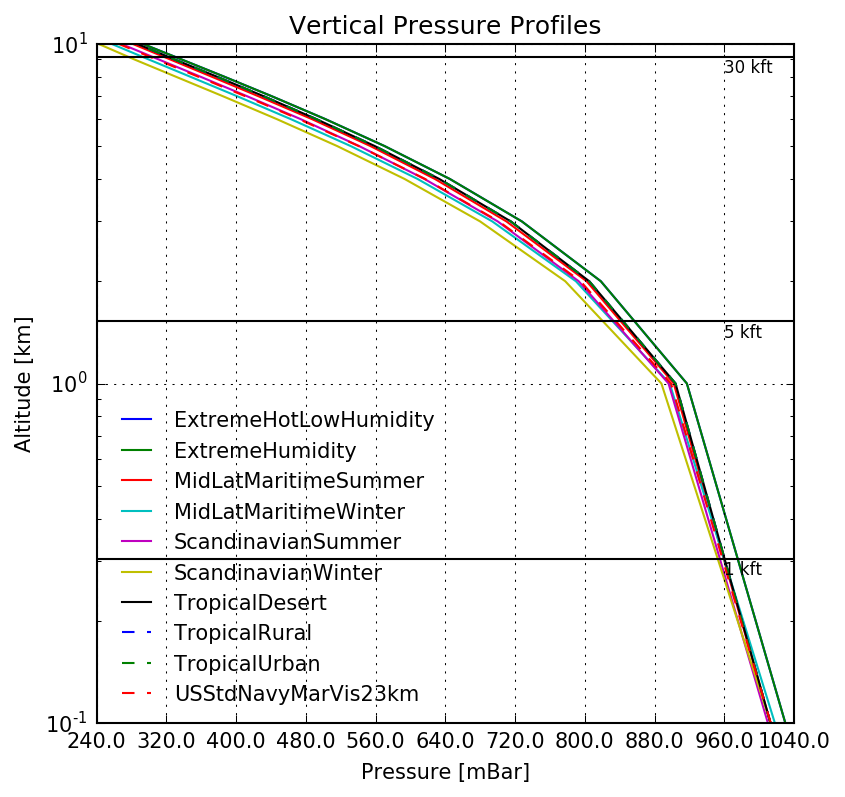
\includegraphics{./pic/Analyse-Standard-Atmospheres_15_0.png}
\end{center}

\begin{center}
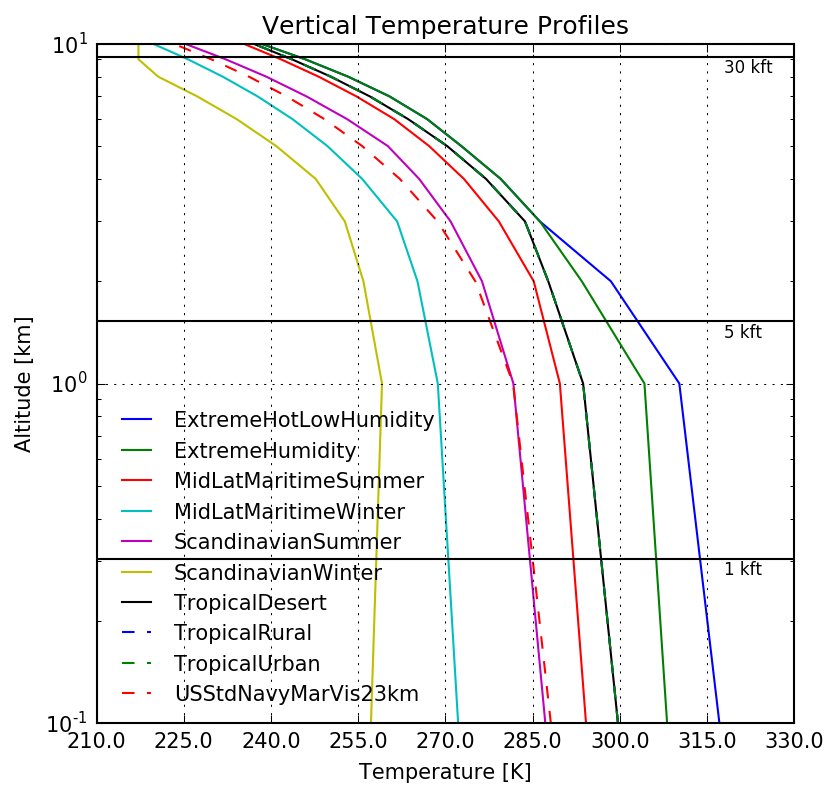
\includegraphics{./pic/Analyse-Standard-Atmospheres_15_1.png}
\end{center}

\begin{center}
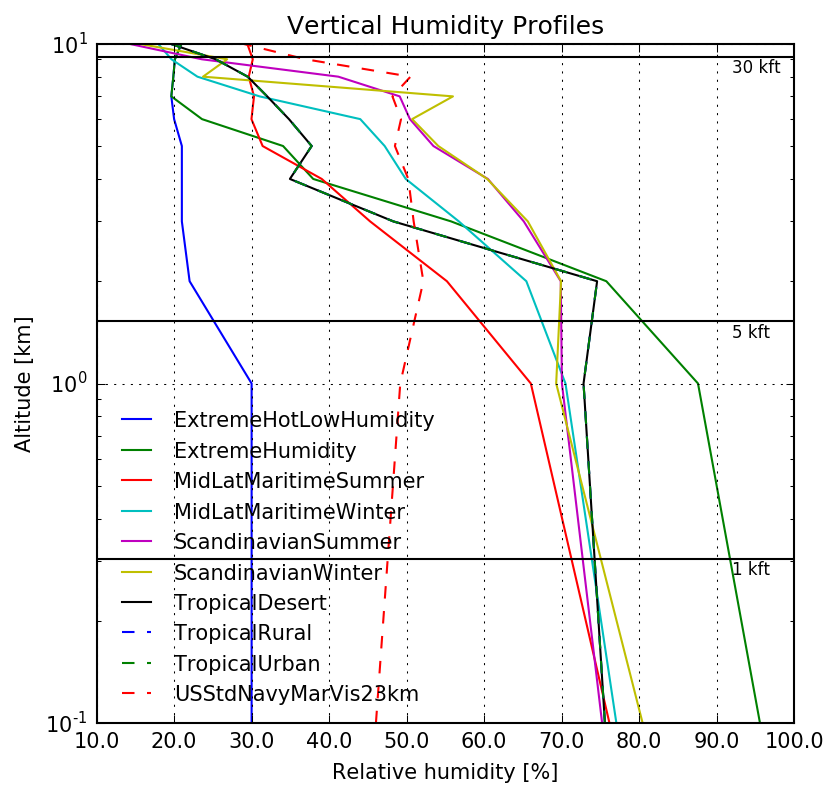
\includegraphics{./pic/Analyse-Standard-Atmospheres_15_2.png}
\end{center}

\begin{center}
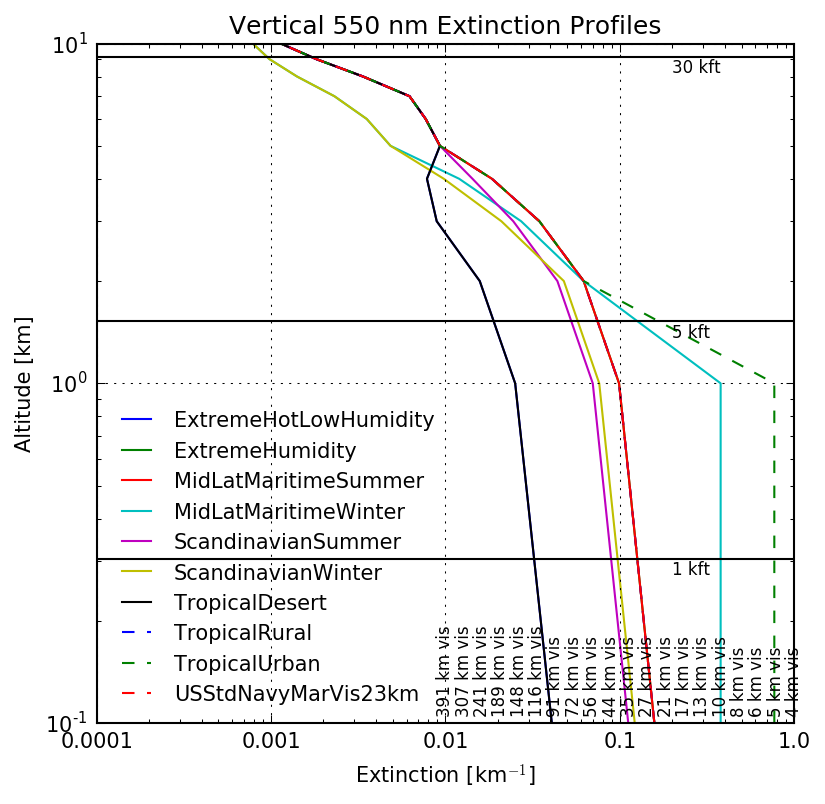
\includegraphics{./pic/Analyse-Standard-Atmospheres_15_3.png}
\end{center}


\section{Spectral Transmittance Plots}
\label{sec:SpectralTransmittancePlots}

Plot the spectral transmittance for 1-km path length. Two sets of plots are shown: 


 1. For each atmosphere, plot the transmittance at different altitudes. 


 2. For shared altitudes, plot the different atmosphere's transmittance.




See Listing~\ref{lst:autolistingcell17} for the code to plot the spectral transmittance.


\begin{lstlisting}[style=outcellstyle]
C:\Miniconda3\envs\py27\lib\site-packages\matplotlib\pyplot.py:516: RuntimeWarning: More than 20 figures have been opened. Figures created through the pyplot interface (`matplotlib.pyplot.figure`) are retained until explicitly closed and may consume too much memory. (To control this warning, see the rcParam `figure.max_open_warning`).
  max_open_warning, RuntimeWarning)

\end{lstlisting}

\begin{center}
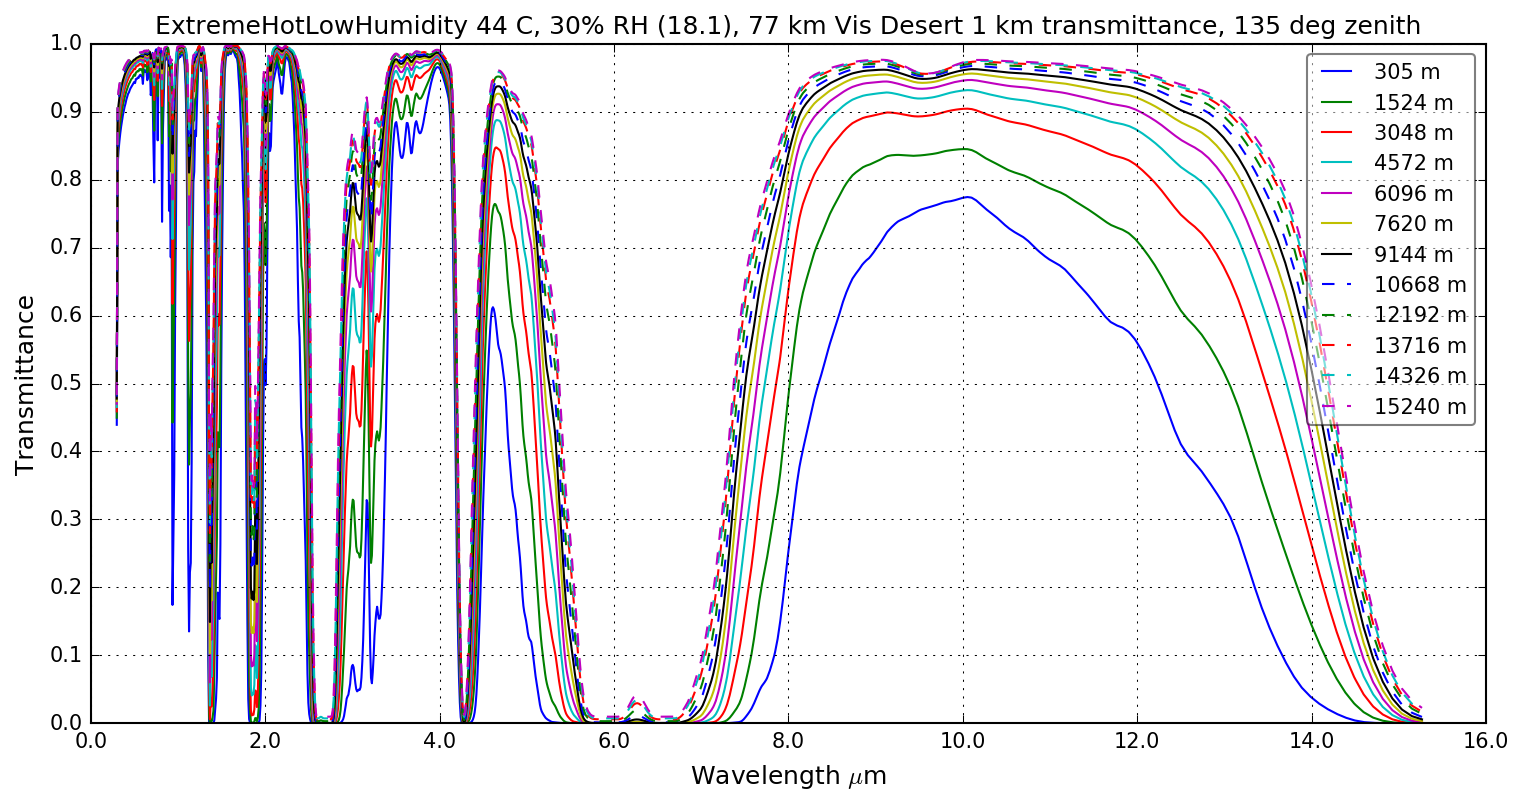
\includegraphics{./pic/Analyse-Standard-Atmospheres_17_1.png}
\end{center}

\begin{center}
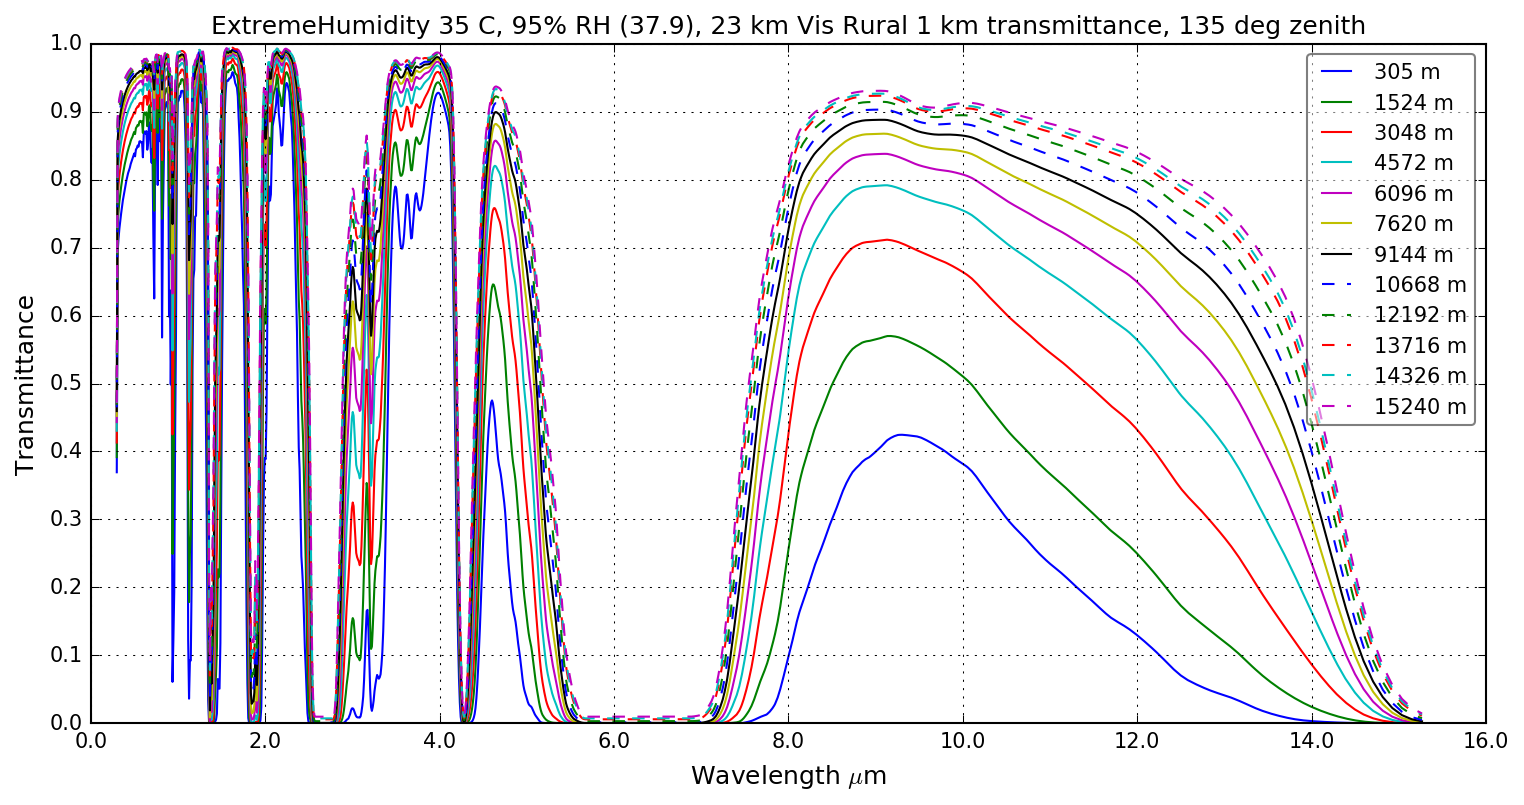
\includegraphics{./pic/Analyse-Standard-Atmospheres_17_2.png}
\end{center}

\begin{center}
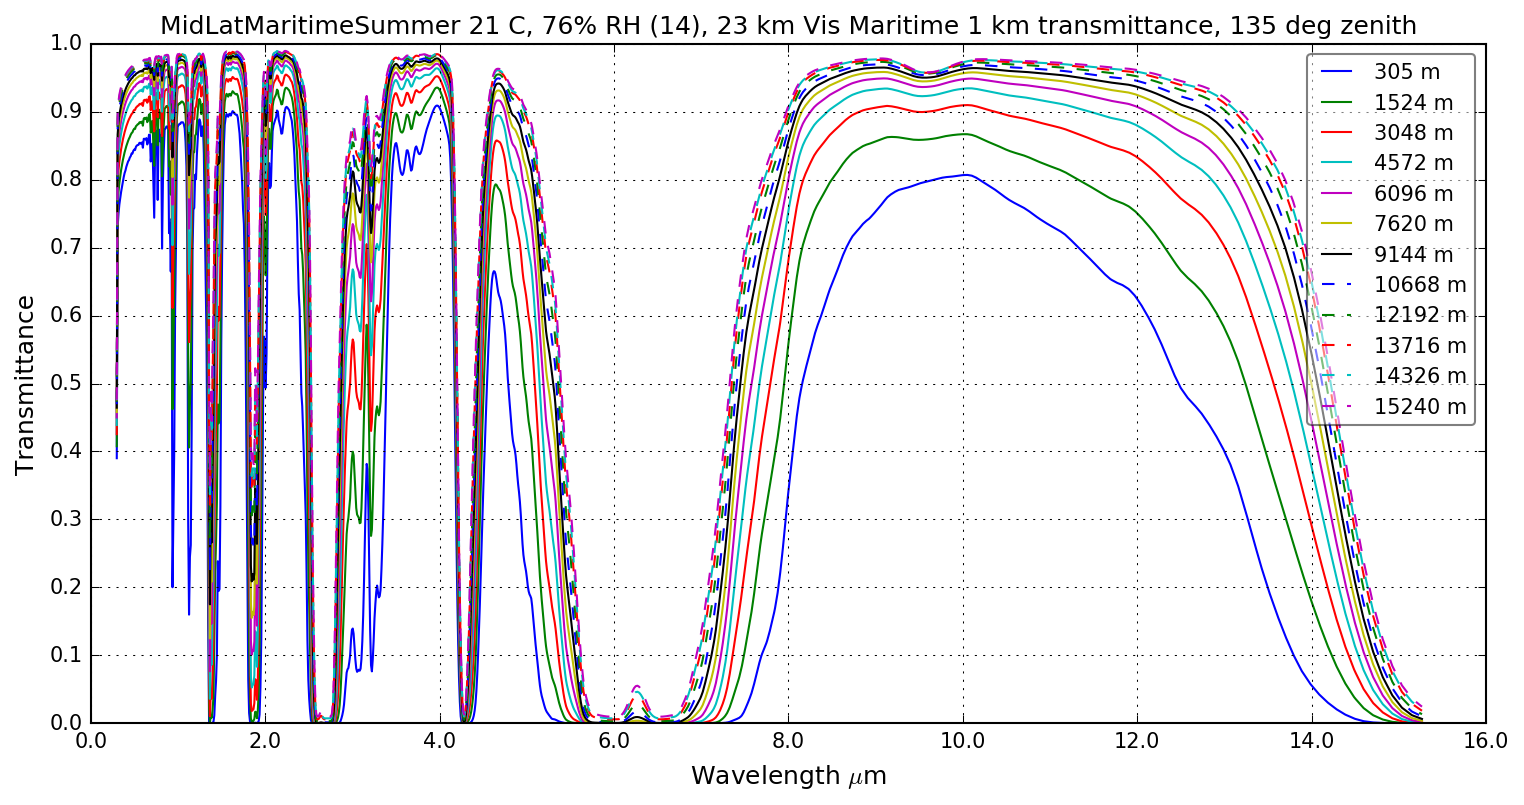
\includegraphics{./pic/Analyse-Standard-Atmospheres_17_3.png}
\end{center}

\begin{center}
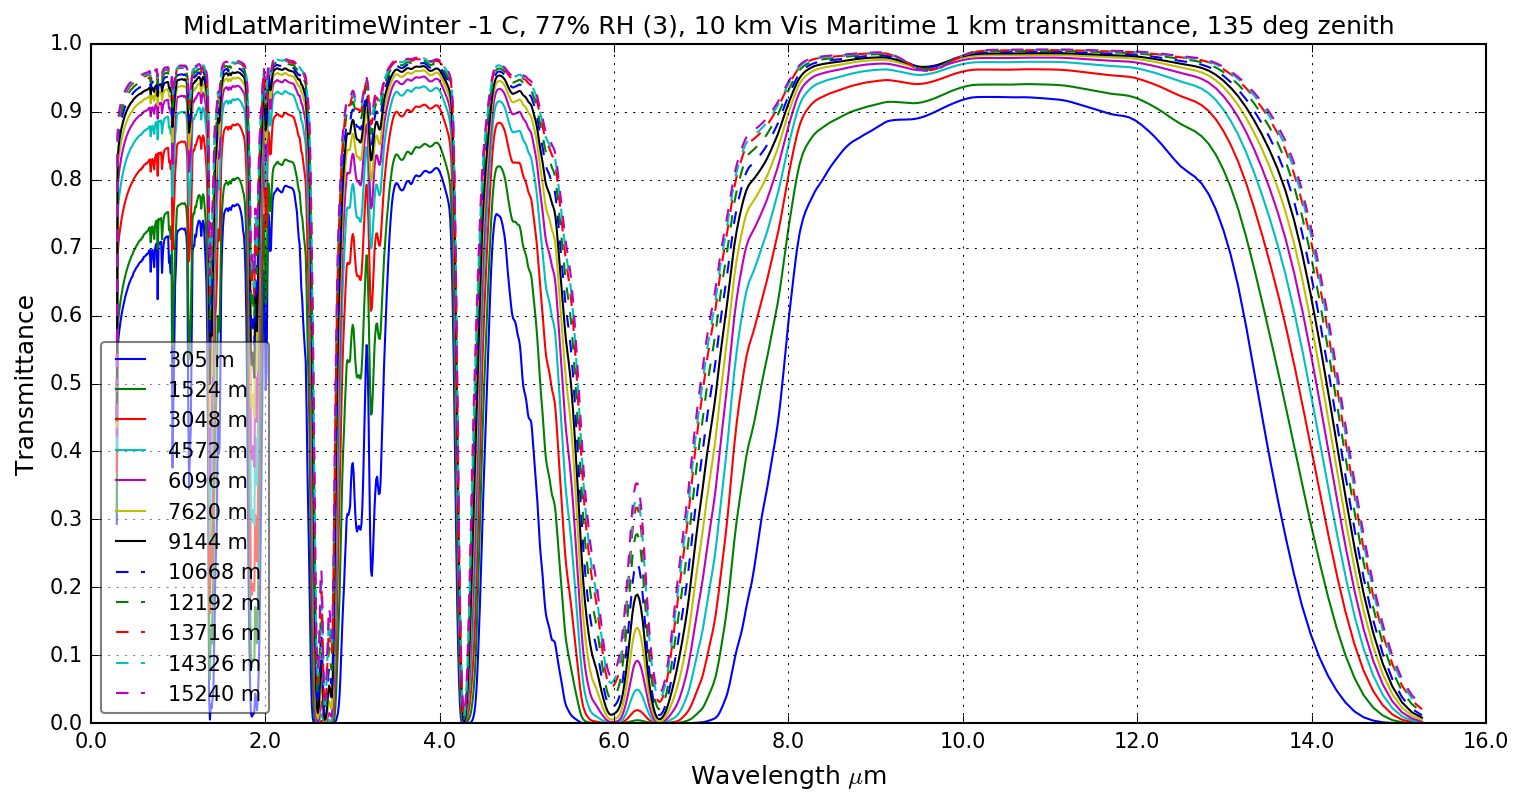
\includegraphics{./pic/Analyse-Standard-Atmospheres_17_4.png}
\end{center}

\begin{center}
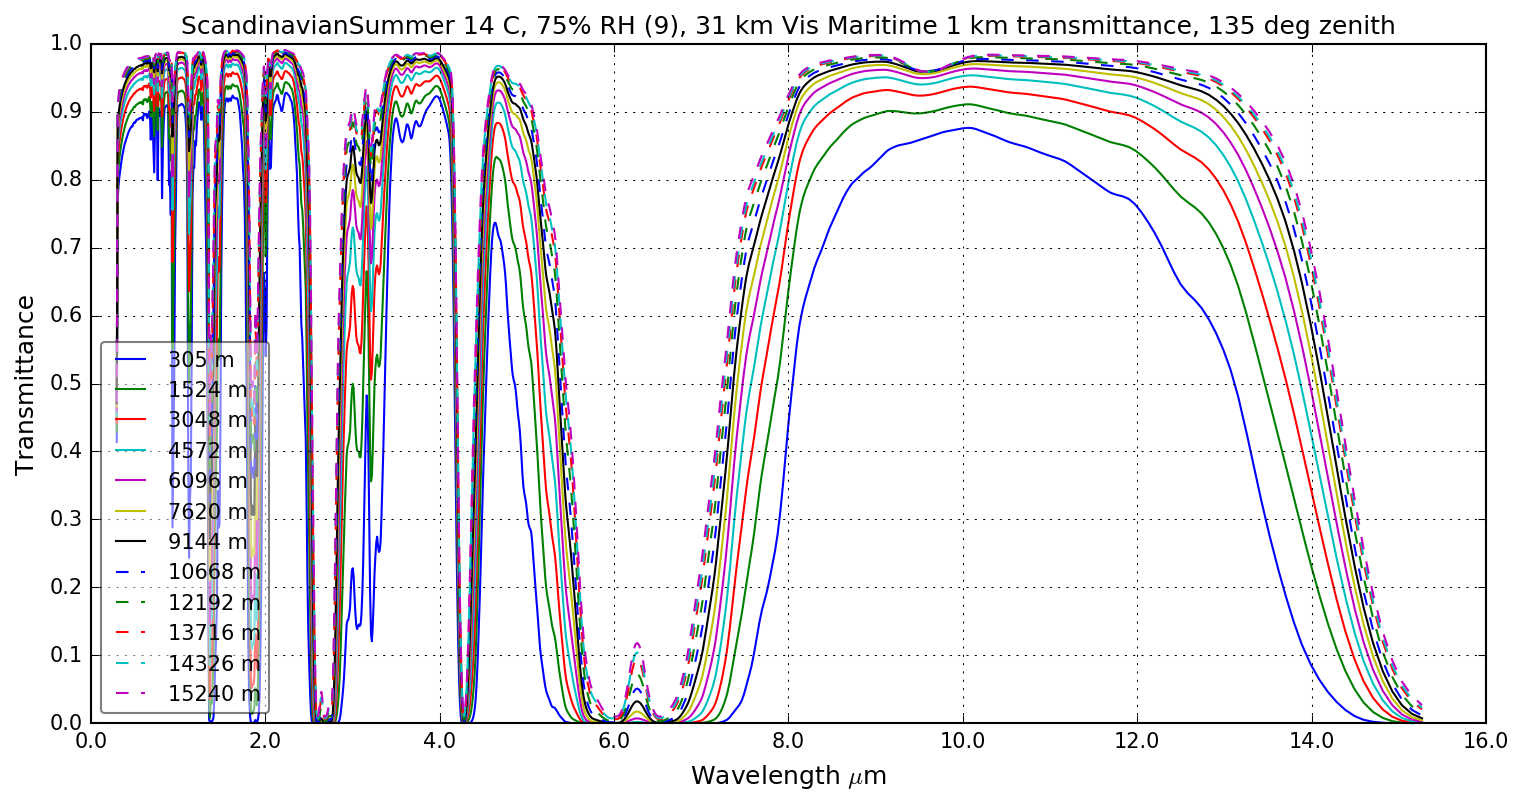
\includegraphics{./pic/Analyse-Standard-Atmospheres_17_5.png}
\end{center}

\begin{center}
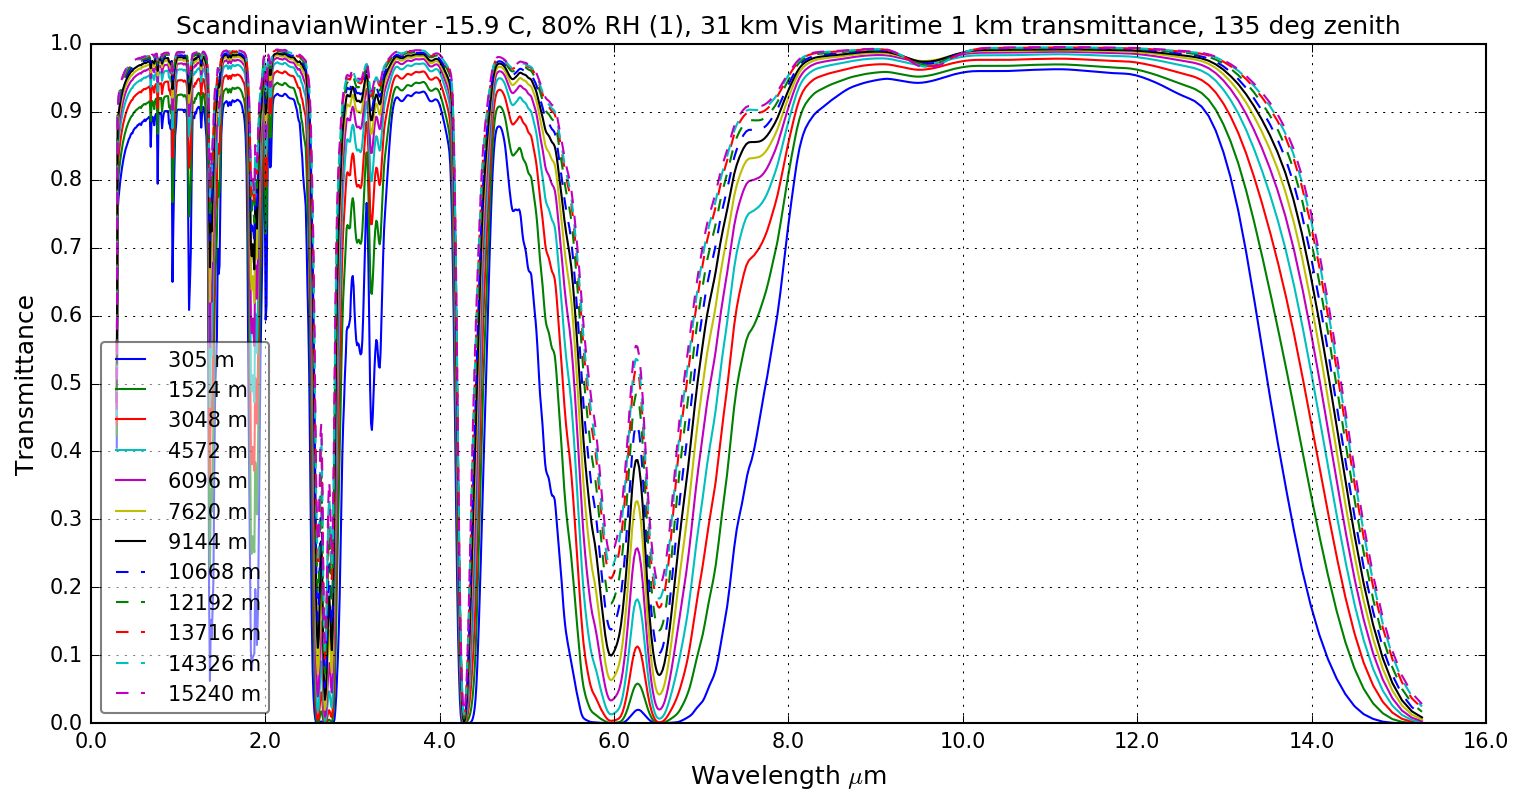
\includegraphics{./pic/Analyse-Standard-Atmospheres_17_6.png}
\end{center}

\begin{center}
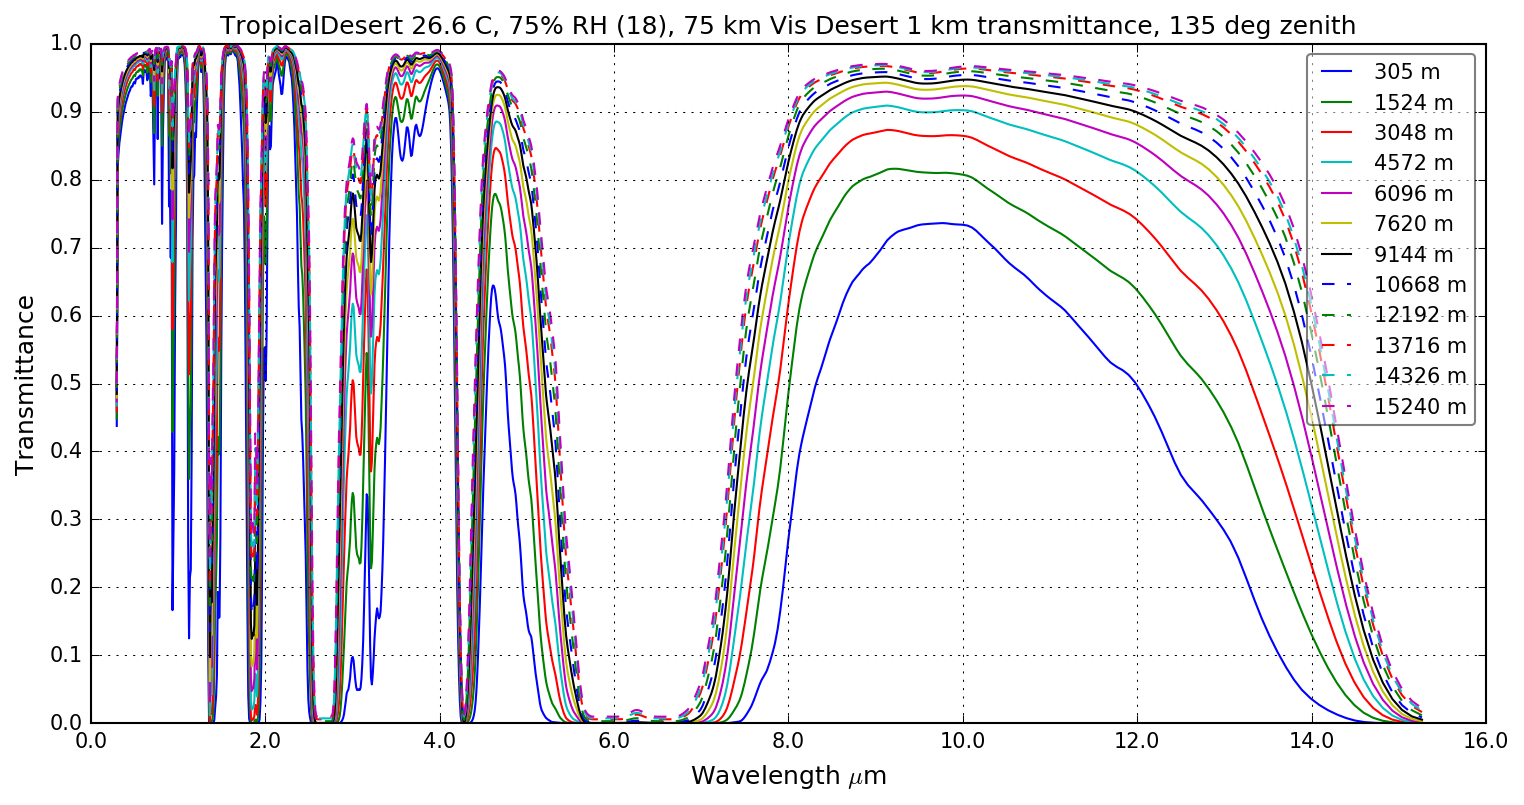
\includegraphics{./pic/Analyse-Standard-Atmospheres_17_7.png}
\end{center}

\begin{center}
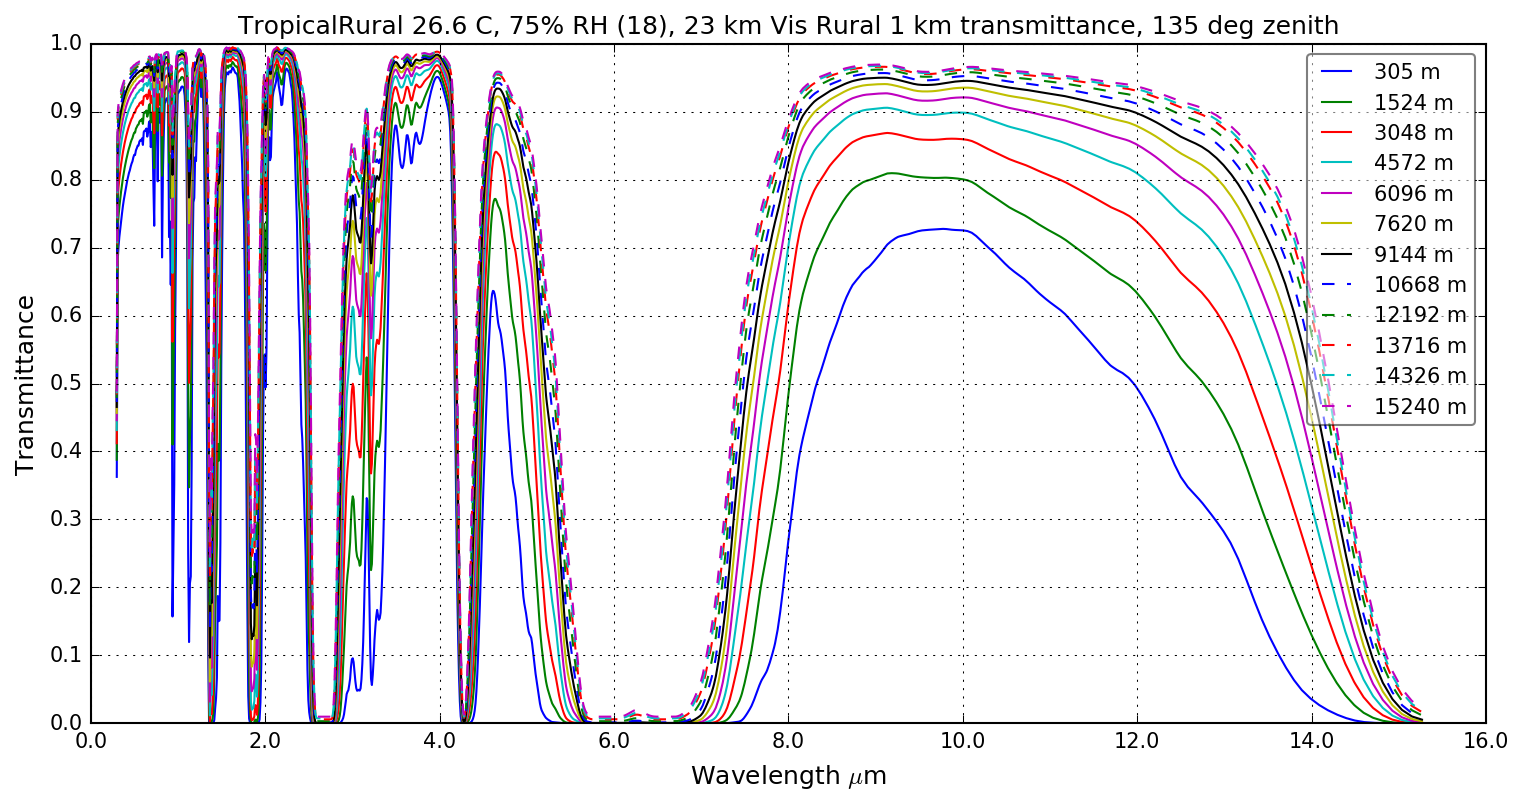
\includegraphics{./pic/Analyse-Standard-Atmospheres_17_8.png}
\end{center}

\begin{center}
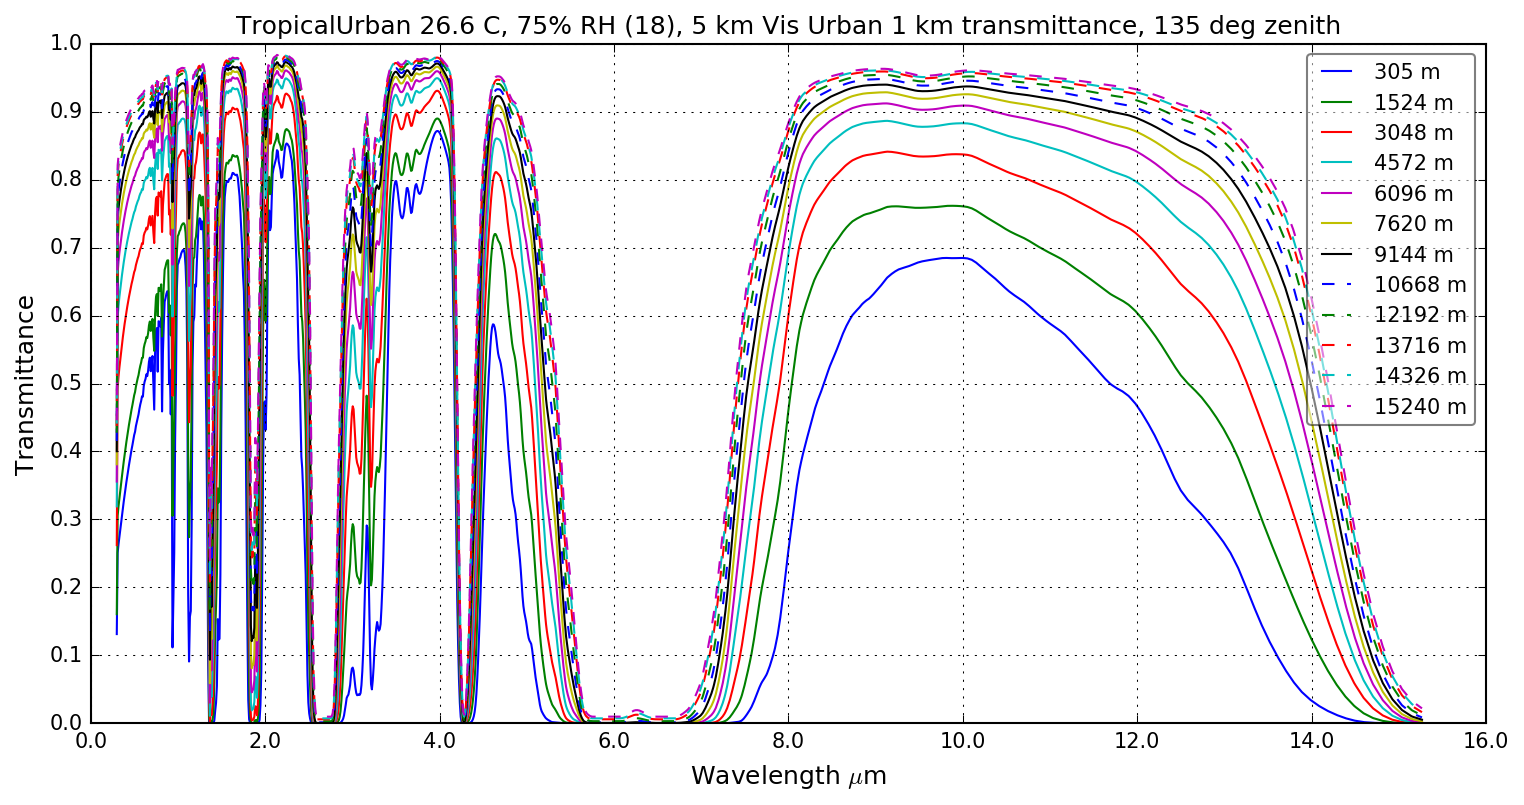
\includegraphics{./pic/Analyse-Standard-Atmospheres_17_9.png}
\end{center}

\begin{center}
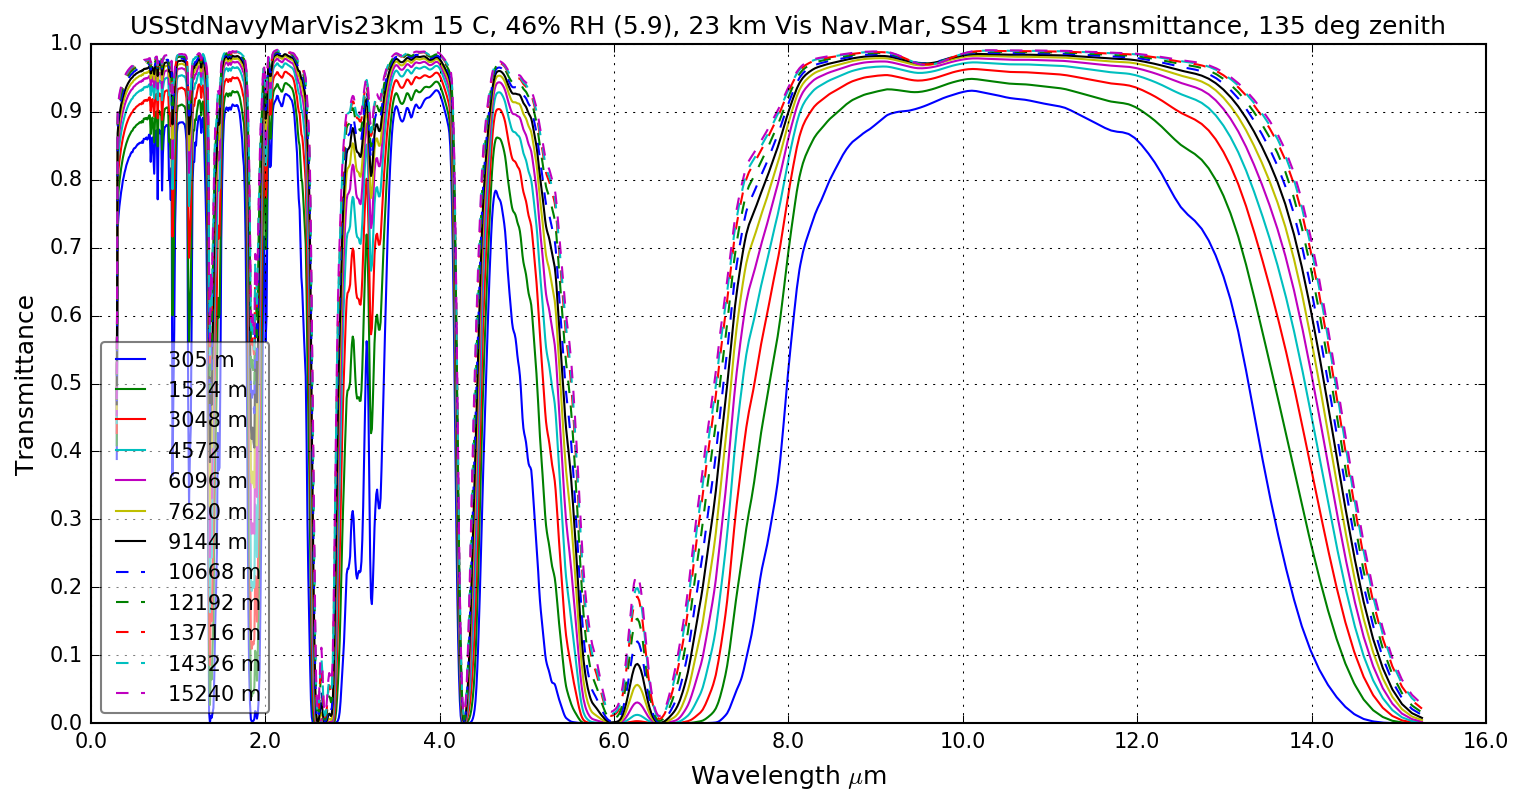
\includegraphics{./pic/Analyse-Standard-Atmospheres_17_10.png}
\end{center}

\begin{center}
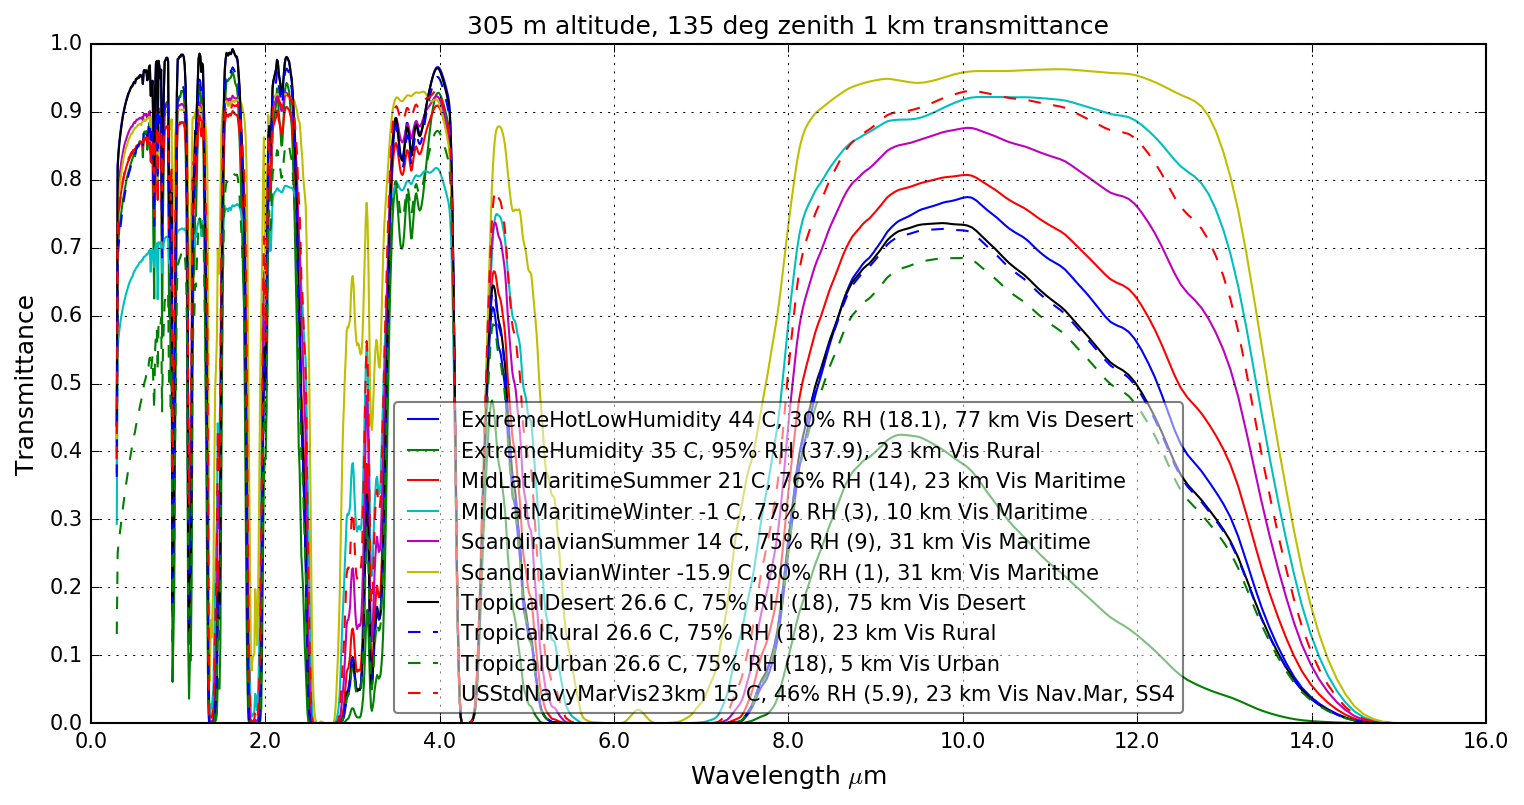
\includegraphics{./pic/Analyse-Standard-Atmospheres_17_11.png}
\end{center}

\begin{center}
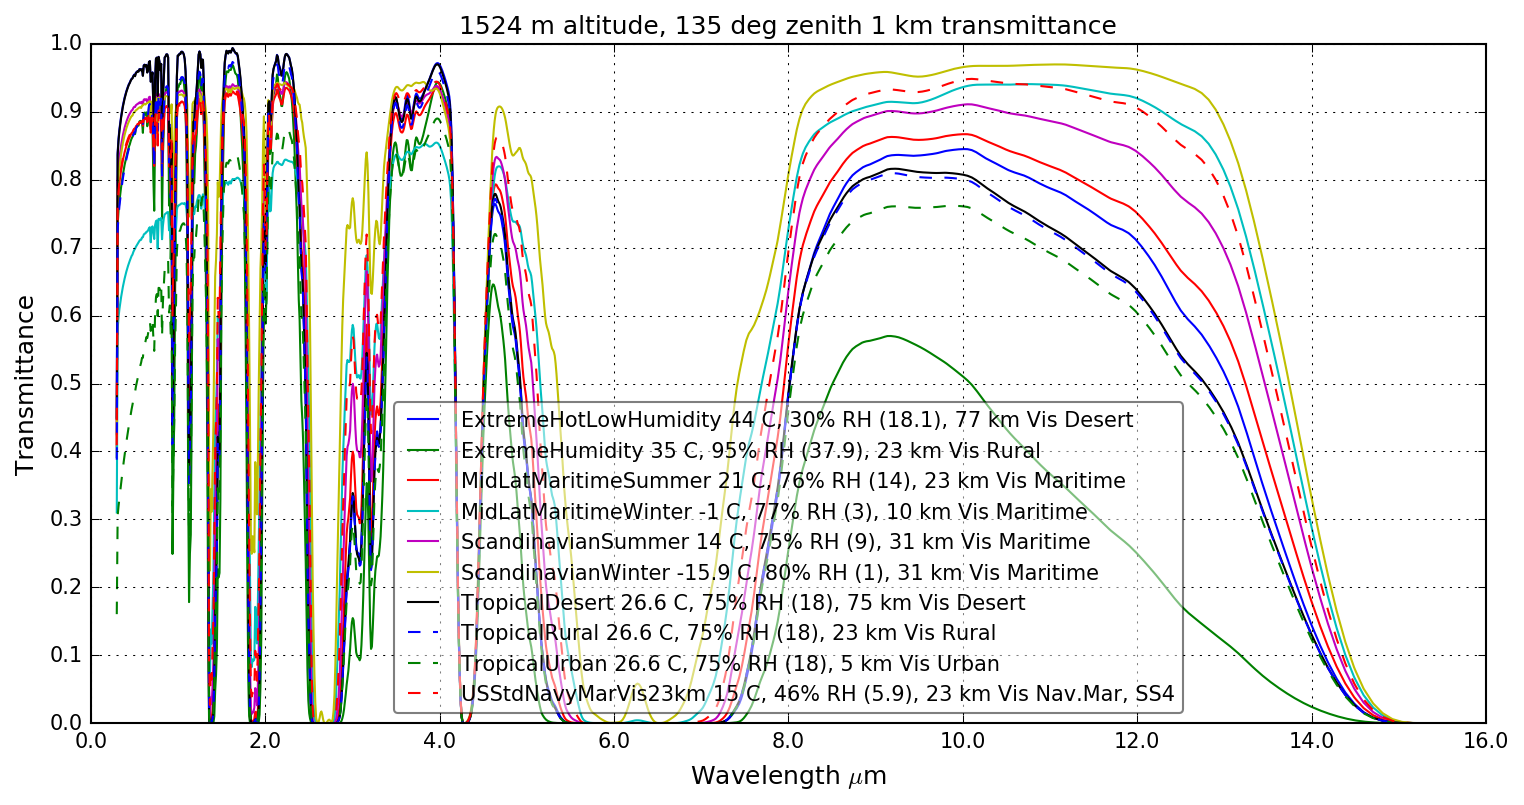
\includegraphics{./pic/Analyse-Standard-Atmospheres_17_12.png}
\end{center}

\begin{center}
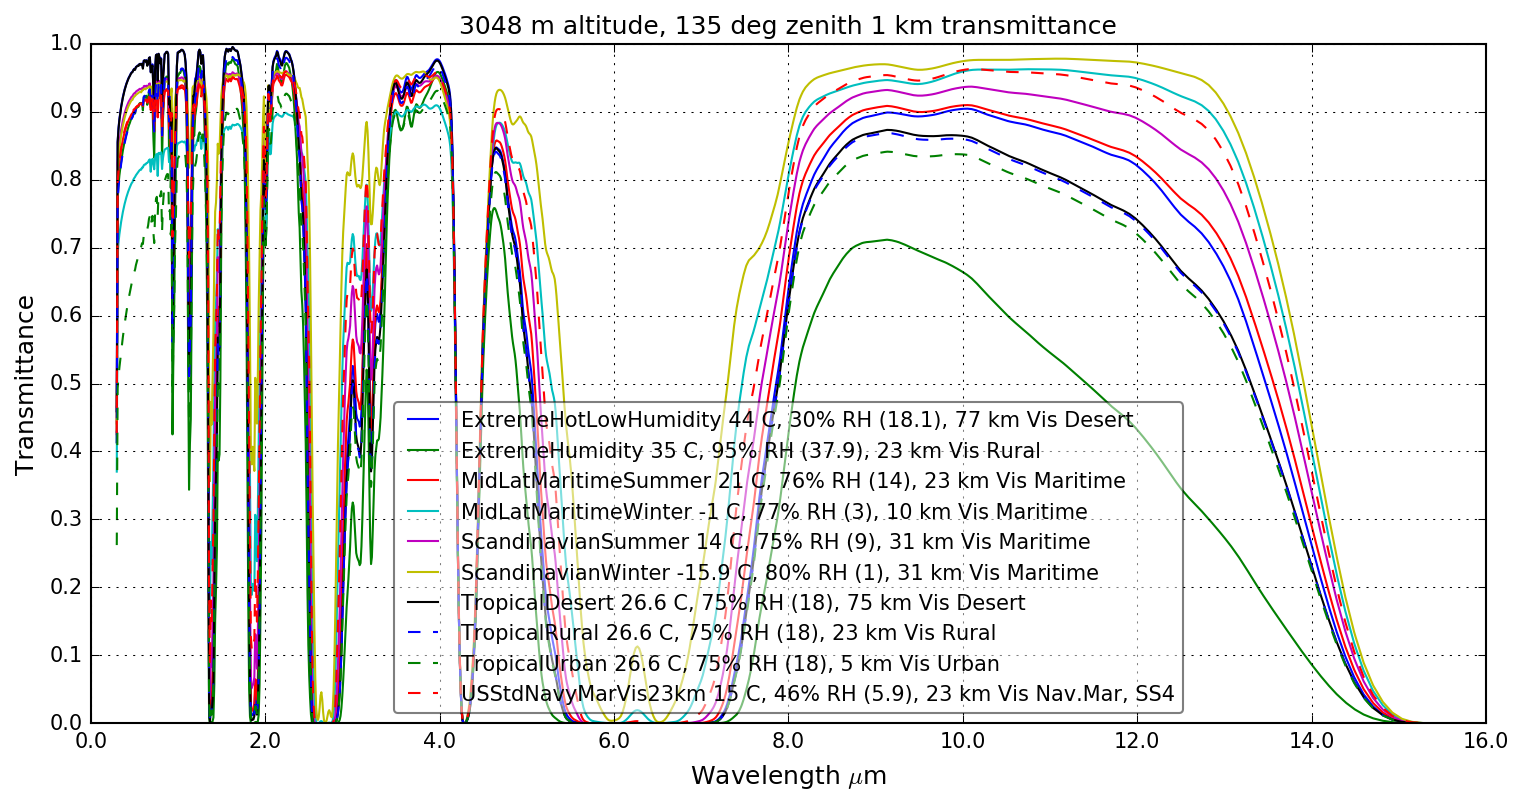
\includegraphics{./pic/Analyse-Standard-Atmospheres_17_13.png}
\end{center}

\begin{center}
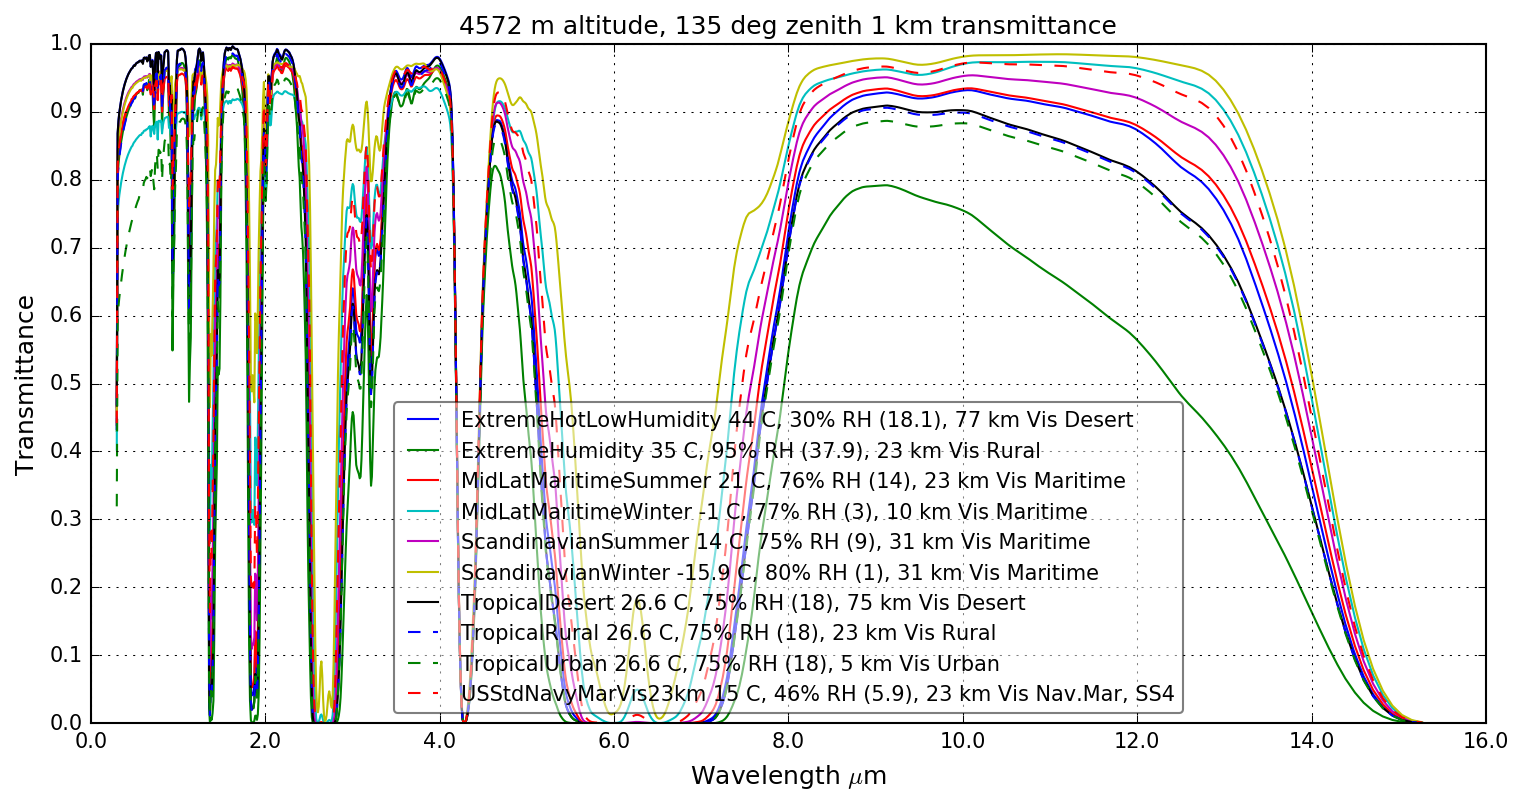
\includegraphics{./pic/Analyse-Standard-Atmospheres_17_14.png}
\end{center}

\begin{center}
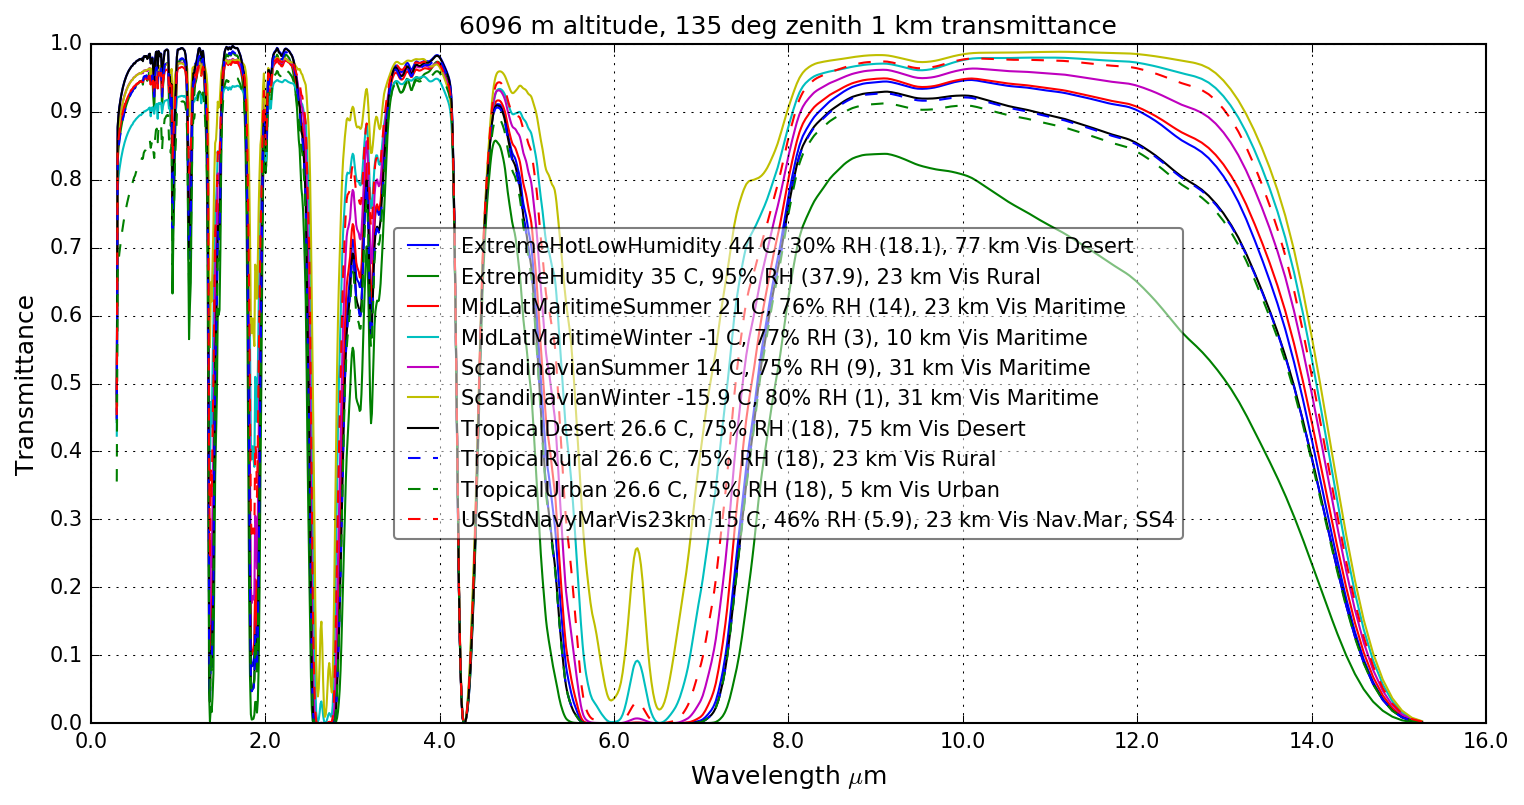
\includegraphics{./pic/Analyse-Standard-Atmospheres_17_15.png}
\end{center}

\begin{center}
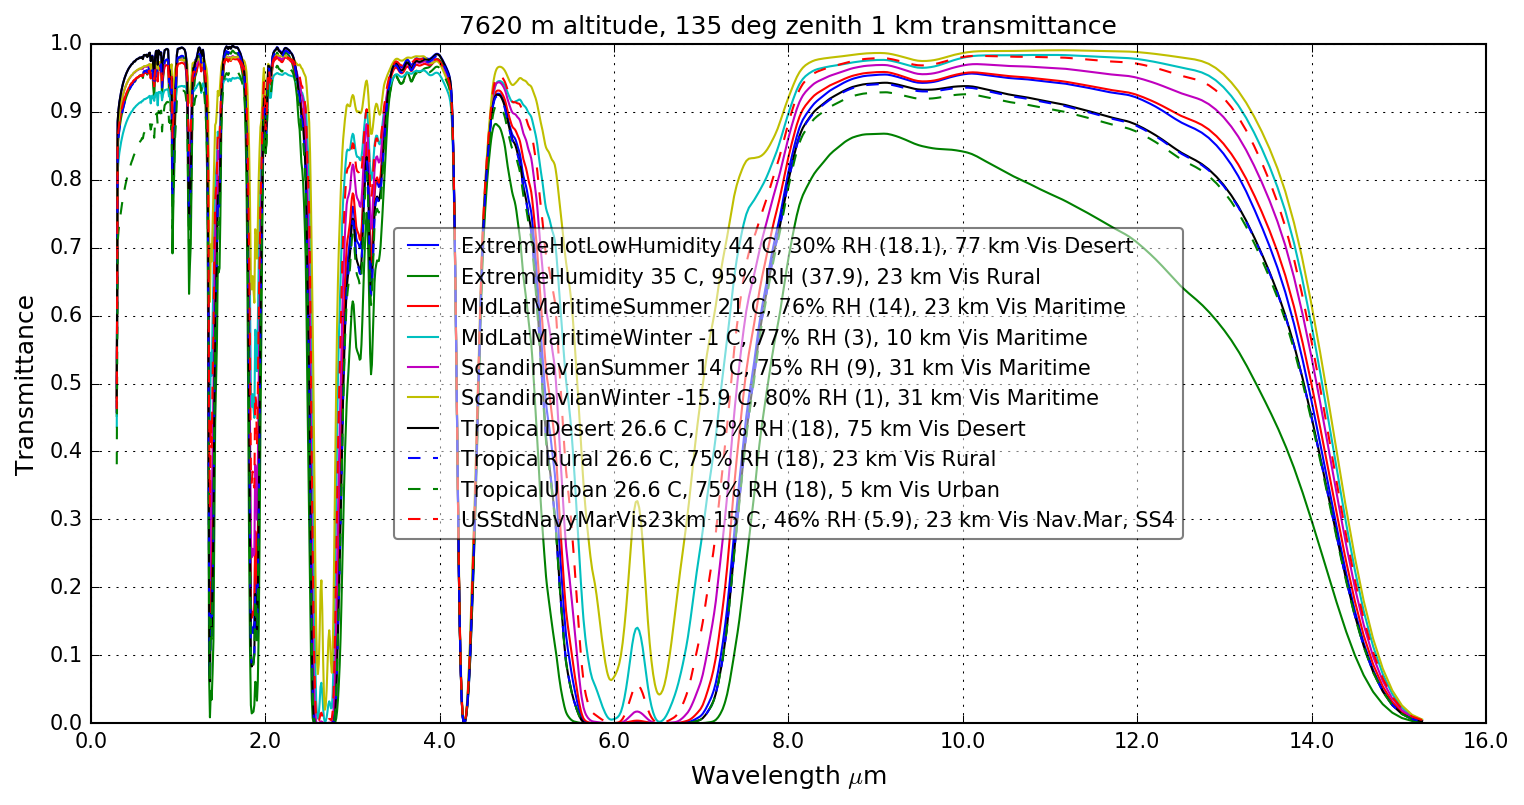
\includegraphics{./pic/Analyse-Standard-Atmospheres_17_16.png}
\end{center}

\begin{center}
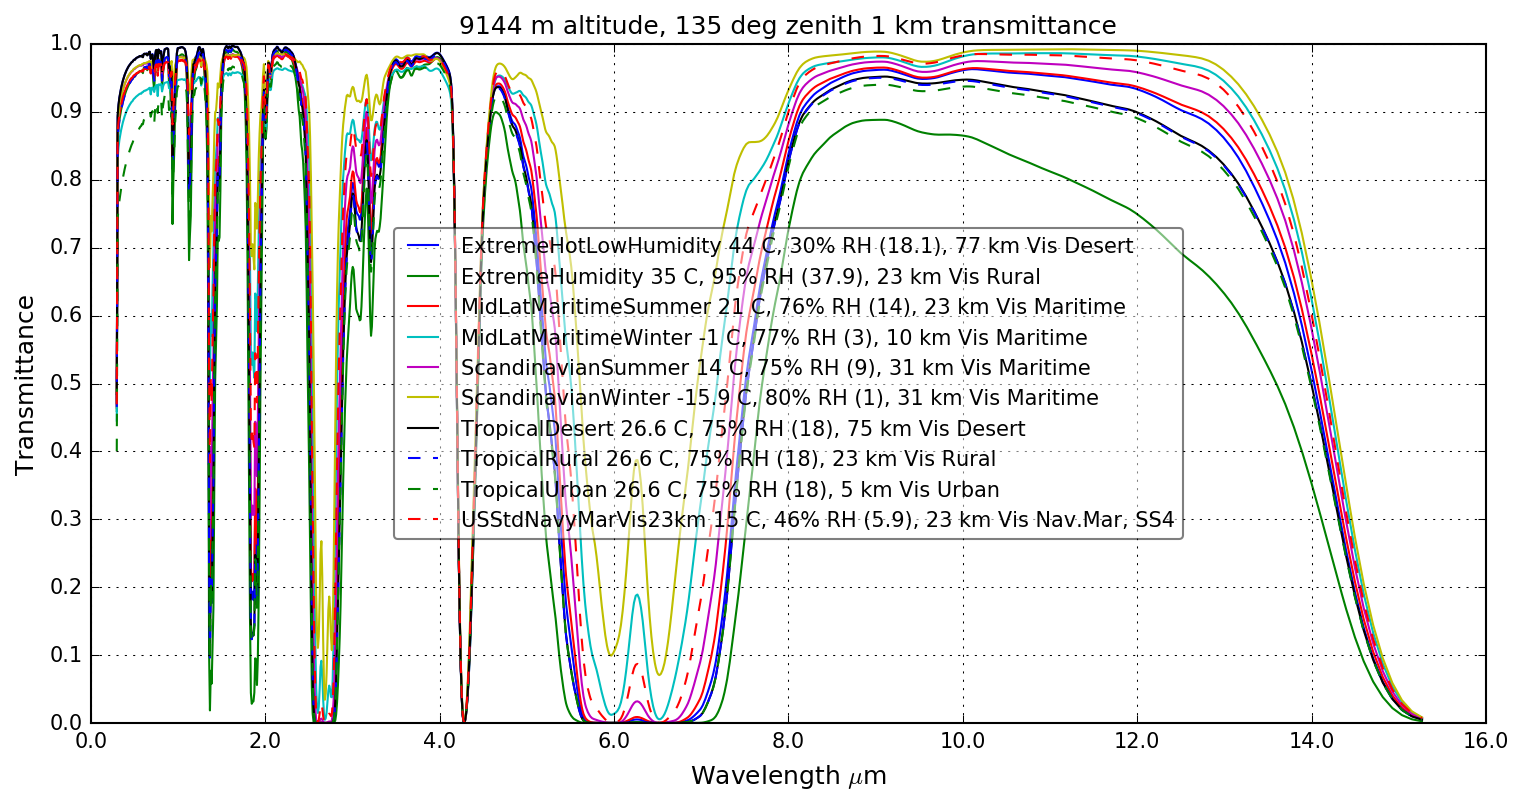
\includegraphics{./pic/Analyse-Standard-Atmospheres_17_17.png}
\end{center}

\begin{center}
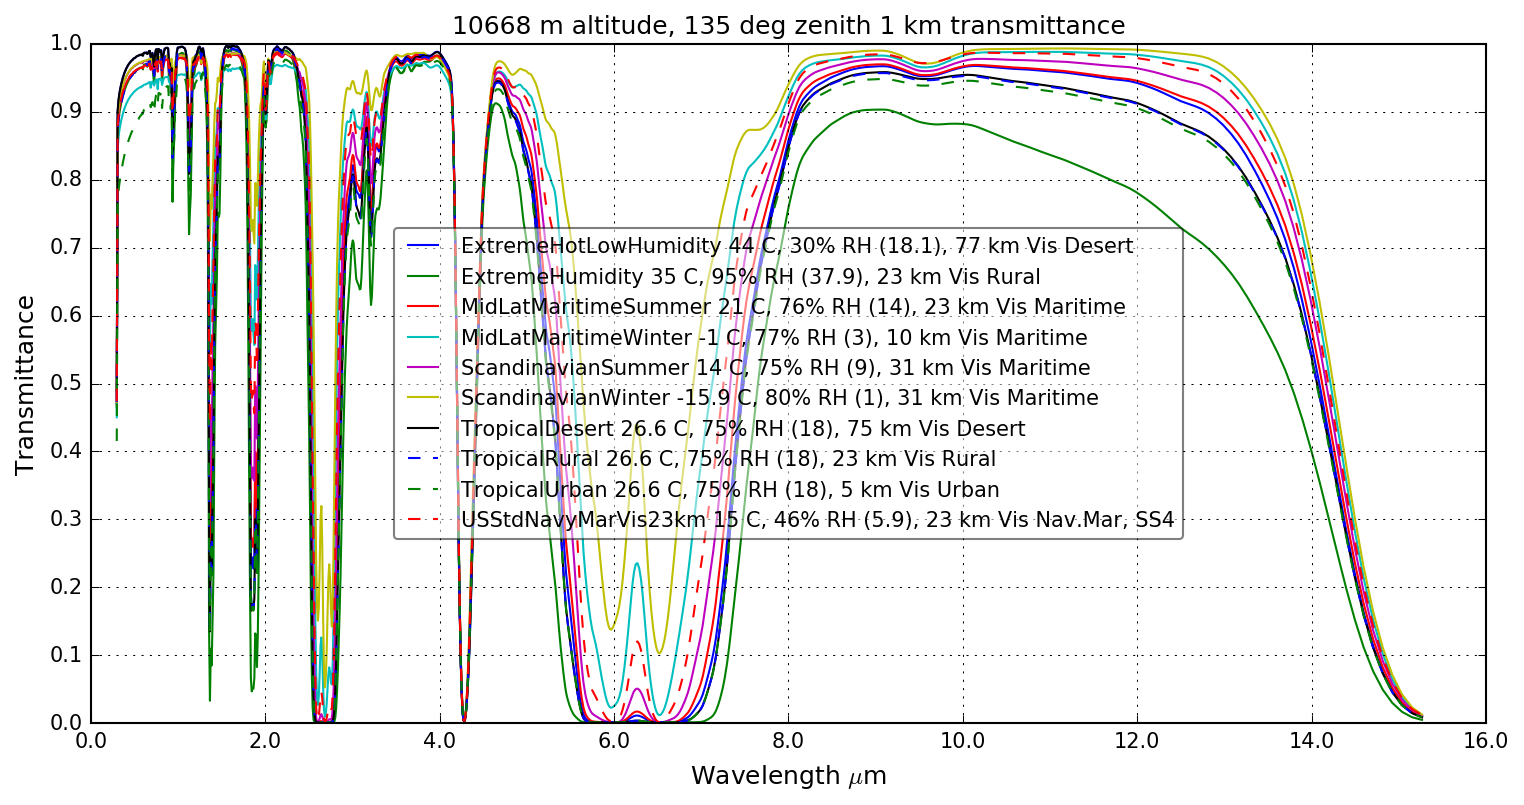
\includegraphics{./pic/Analyse-Standard-Atmospheres_17_18.png}
\end{center}

\begin{center}
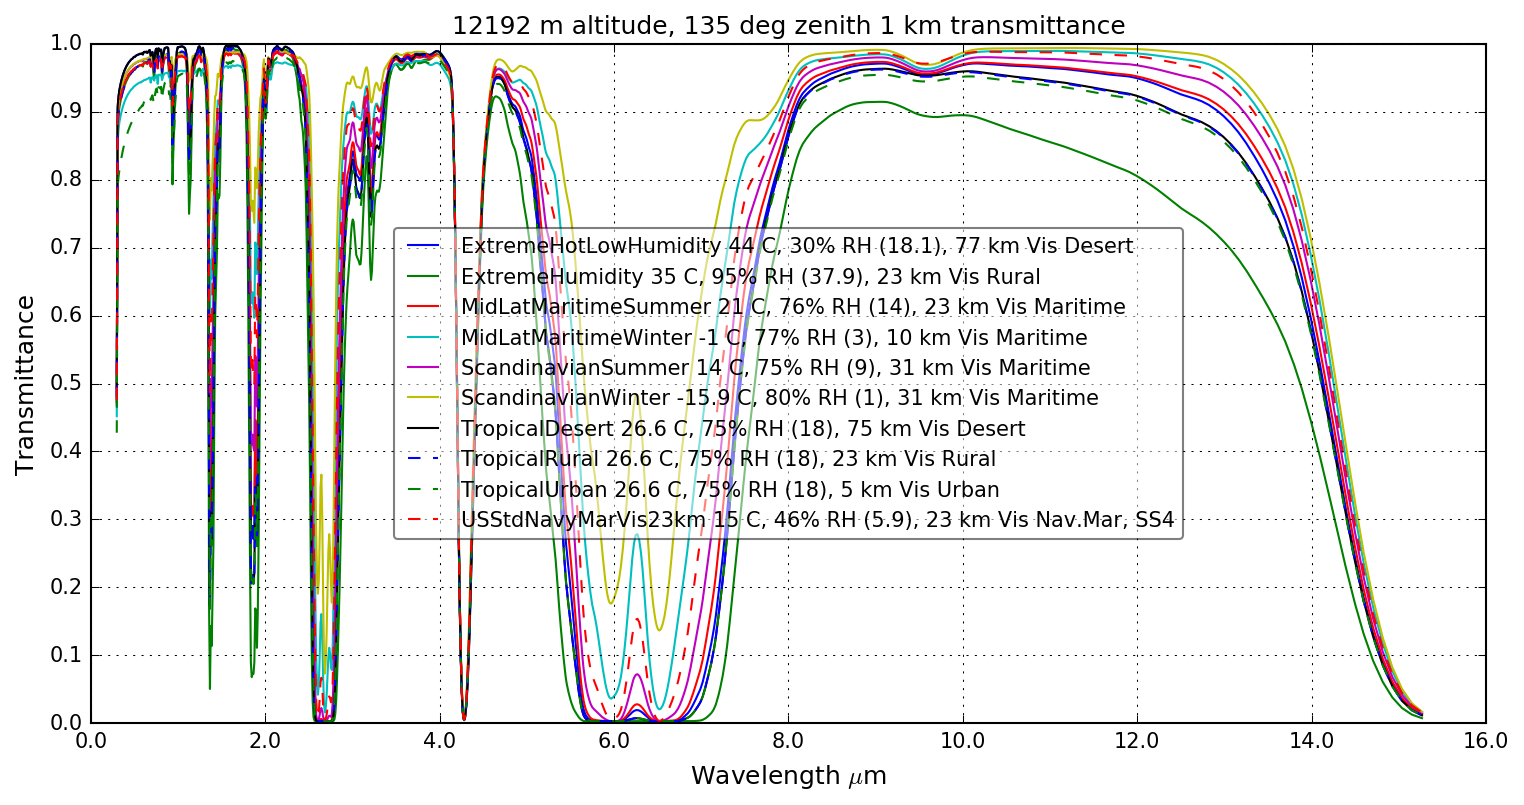
\includegraphics{./pic/Analyse-Standard-Atmospheres_17_19.png}
\end{center}

\begin{center}
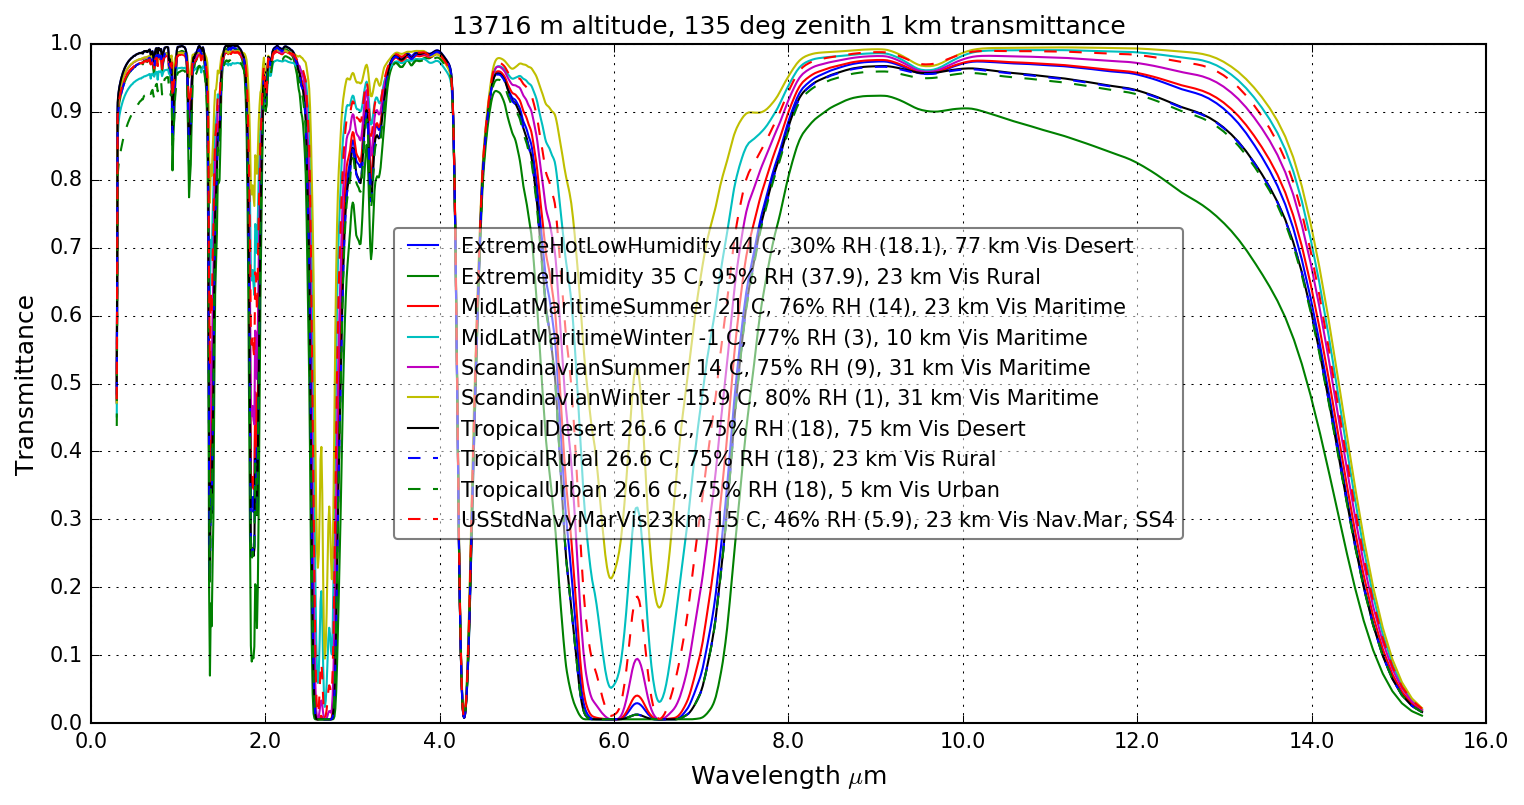
\includegraphics{./pic/Analyse-Standard-Atmospheres_17_20.png}
\end{center}

\begin{center}
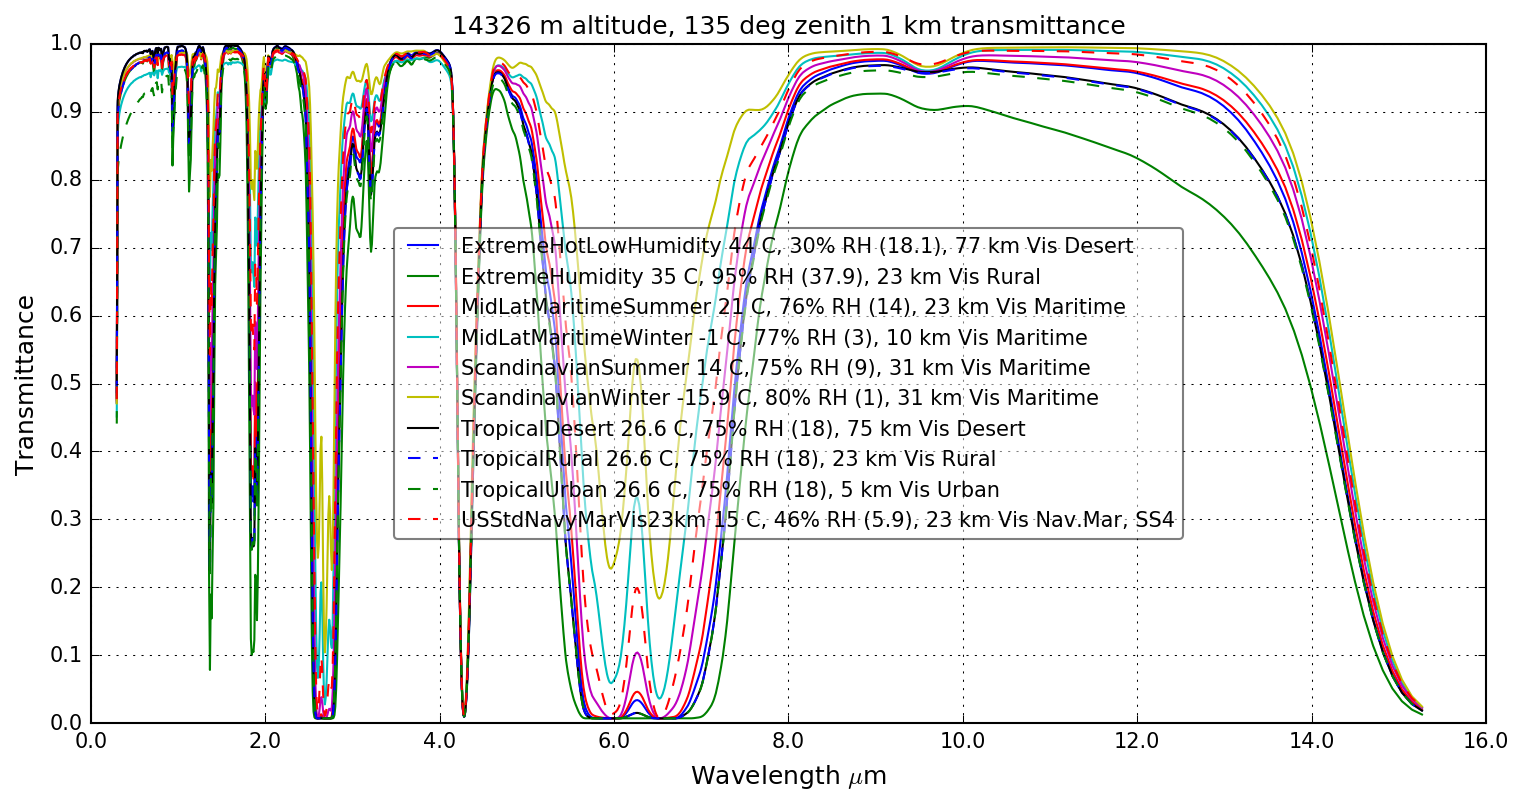
\includegraphics{./pic/Analyse-Standard-Atmospheres_17_21.png}
\end{center}

\begin{center}
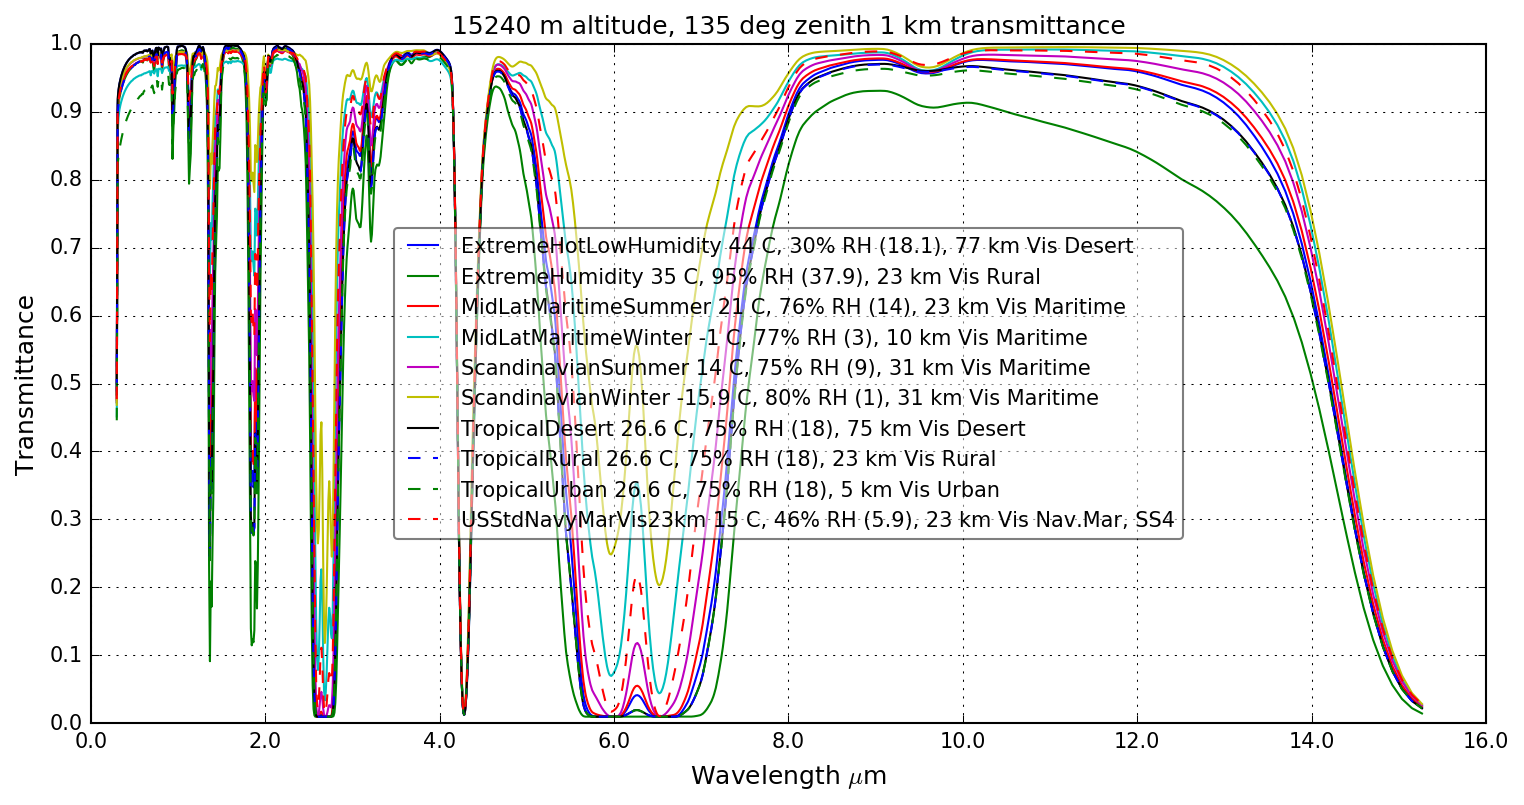
\includegraphics{./pic/Analyse-Standard-Atmospheres_17_22.png}
\end{center}


\section{Apparent Atmospheric Temperature}
\label{sec:ApparentAtmosphericTemperature}

The apparent temperature of the atmosphere is a complex function of the temperature profile along the path.  For slant paths in inhomogeneous atmospheres the effective temperature is affected stronger by the path sections closer to the sensor than path sections further away.


It can be shown that the path radiance in the infrared can be approximated by
\begin{equation}L_\textrm{path} = (1-\tau)\,L(T_\textrm{bb})\end{equation}


This implies that if $L_\textrm{path}$ and $\tau$ are known $T_\textrm{bb}$ can be determined.  The solution is determined by fitting a curve of the above shape to the Modtran-calculated path radiance, finding $T_\textrm{bb}$ for the best fit.  Only the thermal path radiance is used, which has most of its optical flux at wavenumbers below 2500 cm$^{-1}$.


The analysis below considers three spectral bands: (1) a band in the 3.5-4.8 $\mu$m range, (1) a band in the 8.3-12 $\mu$m range, and (3) a band that covers \textit{four} windows in the 3.2-12.5 $\mu$m range.


It turns out that the temperatures calculated for the 3.5-4.8 $\mu$m band is similar to the average or broadband temperature, because of the mix of CO$_2$ absorption and good transmittance in this band.


At low altitudes all the atmospheric temperatures are similar but at high altitudes there can be a significant spread in the values.


The term 'best fit' is not easily defined.  It is not clear what a simple fit through all the data really mean.  Several options were considered: (1) use only the spectral ranges with high transmittance, (2) use only the spectral ranges with poor transmittance, (3) use all the data, and (4) calculate the mean value of the first two options.
The results of these two approaches are shown below in the example graphs.  The temperatures calculated from all the data and the mean of the high and low transmittance temperatures are broadly in agreement.


If the apparent atmosphere temperatures are used in applications where the path radiance in the atmospheric windows are required, it is proposed that the 'high transmittance' temperature values be used. These values will be more applicable to the in-band path radiance.


The results shown in the graphs and tables below are for the following conditions:


\begin{center}

\begin{normalsize}

\begin{tabular}{|c|c|}
\hline
Heading&Meaning\\\hline
TmpLoTau&Apparent temperature in all spectral ranges with low transmittance\\\hline
TmpHiTau&Apparent temperature in all spectral ranges with high transmittance\\\hline
3.5-4.8&Apparent temperature in the full spectral band (including absorption)\\\hline
8.3-12&Apparent temperature in the full spectral band (including absorption)\\\hline
TmpAve&Arithmetic Average (TmpLoTau+TmpHiTau)/2\\\hline
TmpAll&Apparent temperature over the total spectral range\\\hline

\end{tabular}
\end{normalsize}
\end{center}



See Listing~\ref{lst:autolistingcell20} for the code to return Placnk radiator radiance.



See Listing~\ref{lst:autolistingcell21} for the code to calculate and plot atmospheric temperature.

\begin{center}
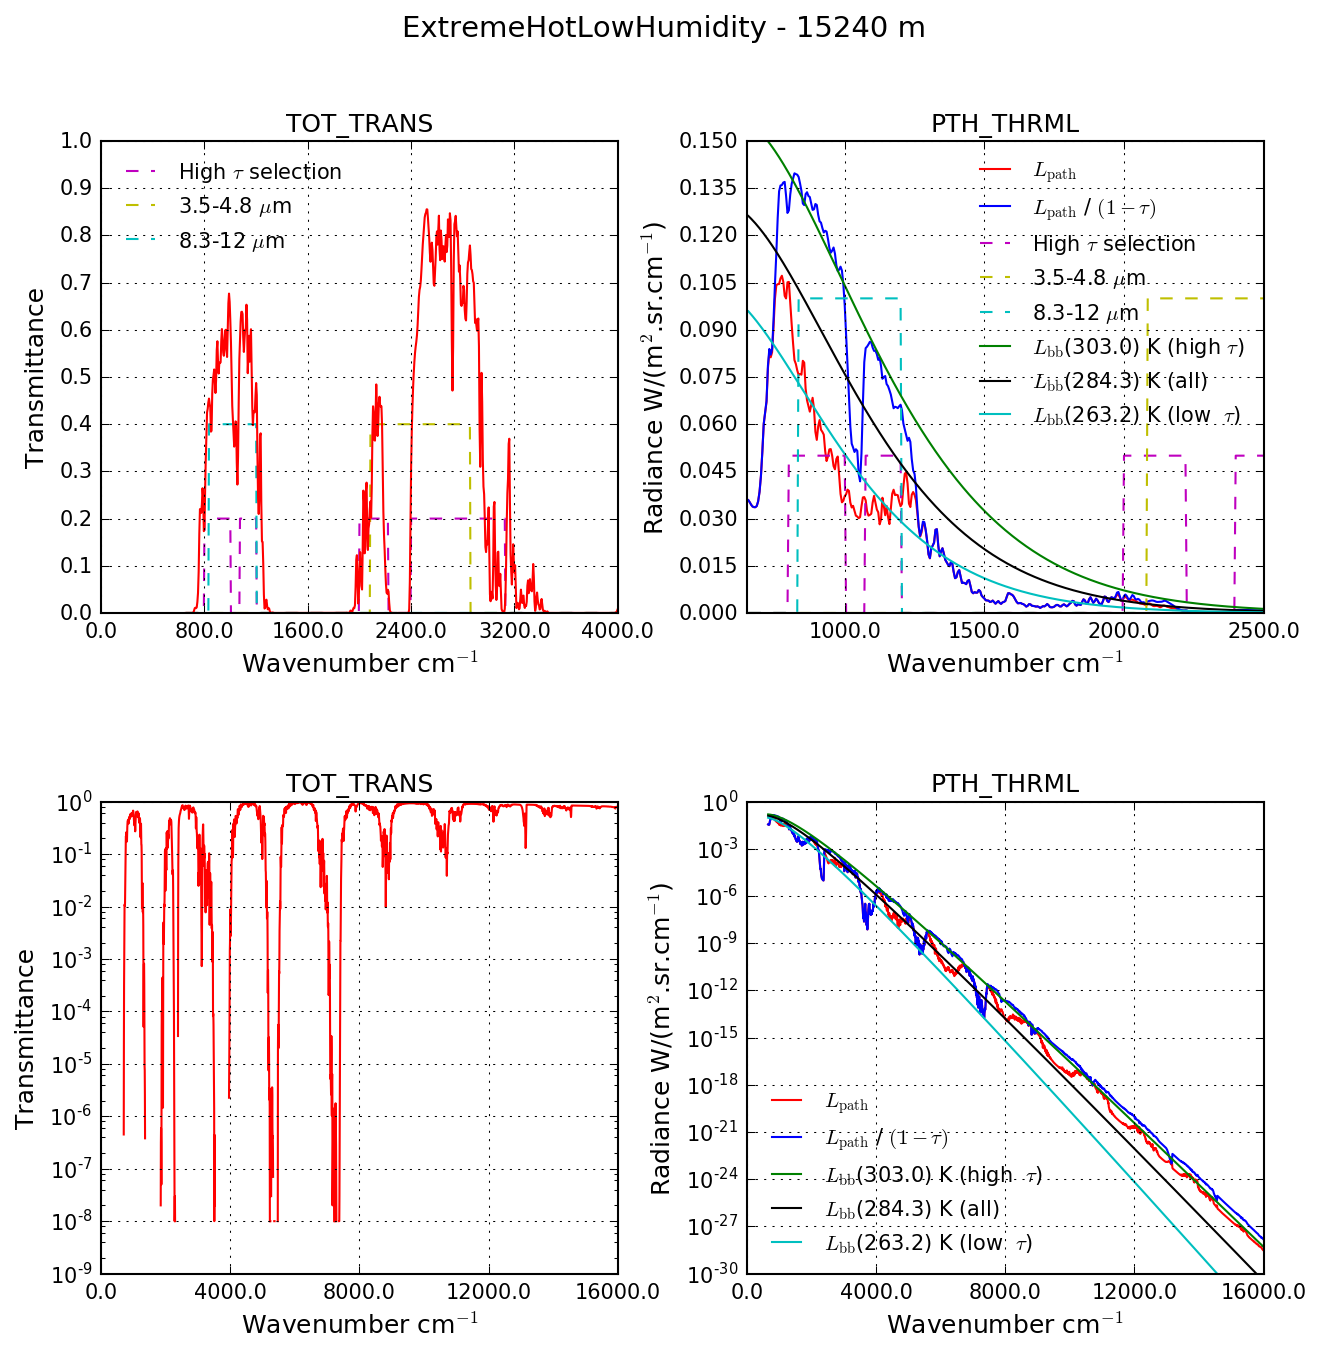
\includegraphics{./pic/Analyse-Standard-Atmospheres_21_0.png}
\end{center}

\begin{center}
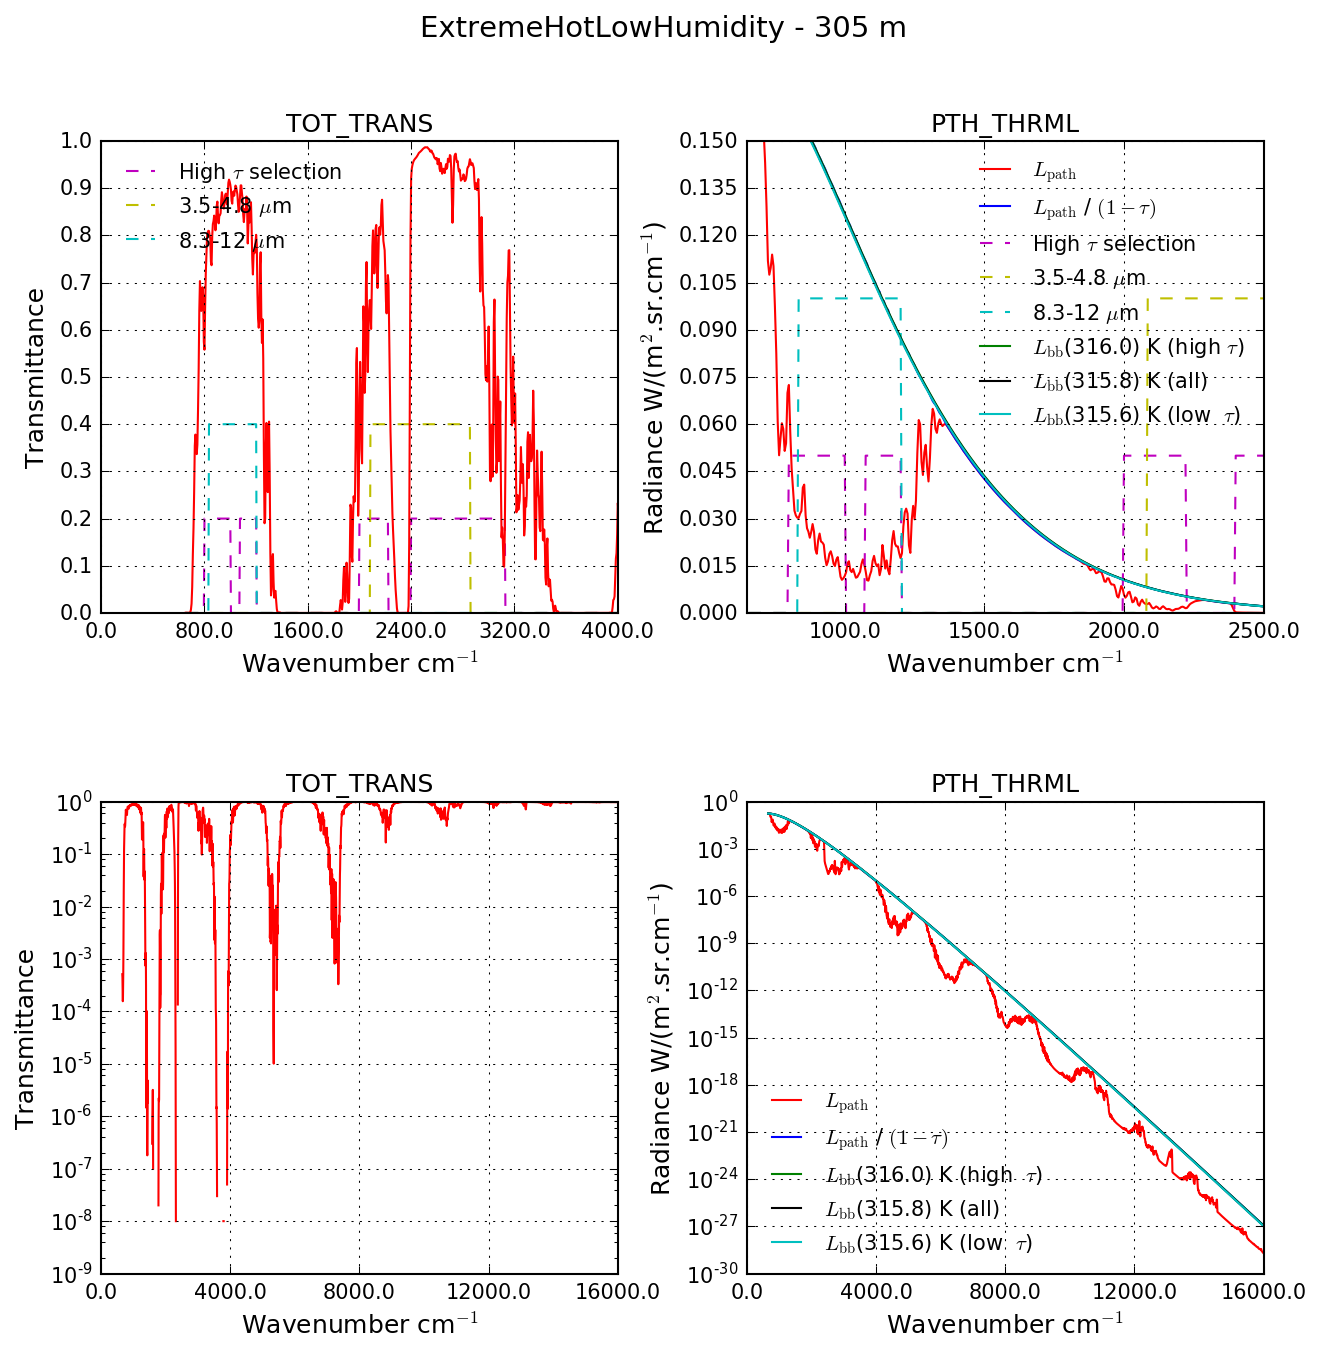
\includegraphics{./pic/Analyse-Standard-Atmospheres_21_1.png}
\end{center}



See Listing~\ref{lst:autolistingcell22} for the code to process and print atmospheric transmittance.

\begin{center}

\begin{normalsize}

\begin{tabular}{|c|c|c|c|c|c|c|c|}
\hline
&Altitude&TmpLoTau&TmpHiTau&3.5-4.8&8.3-12&TmpAve&TmpAll\\\hline
Atmosphere&&&&&&&\\\hline
ExtremeHotLowHumidity&305.0&315.6&316.0&315.8&316.0&315.8&315.8\\\hline
ExtremeHotLowHumidity&1524.0&307.7&311.3&309.5&311.4&309.5&309.4\\\hline
ExtremeHotLowHumidity&3048.0&296.5&307.3&300.7&307.4&301.9&301.6\\\hline
ExtremeHotLowHumidity&4572.0&290.0&305.6&295.5&305.4&297.8&297.5\\\hline
ExtremeHotLowHumidity&6096.0&284.9&304.6&291.9&304.1&294.7&294.5\\\hline
ExtremeHotLowHumidity&7620.0&280.3&304.0&289.4&303.1&292.2&292.1\\\hline
ExtremeHotLowHumidity&9144.0&276.0&303.7&287.5&302.3&289.8&289.9\\\hline
ExtremeHotLowHumidity&10668.0&272.1&303.5&286.1&301.4&287.8&288.2\\\hline
ExtremeHotLowHumidity&12192.0&268.6&303.3&285.2&300.6&286.0&286.6\\\hline
ExtremeHotLowHumidity&13716.0&265.6&303.1&284.5&299.6&284.4&285.3\\\hline
ExtremeHotLowHumidity&14326.0&264.5&303.1&284.3&299.2&283.8&284.8\\\hline
ExtremeHotLowHumidity&15240.0&263.1&303.0&284.0&298.7&283.0&284.2\\\hline

\end{tabular}
\end{normalsize}
\end{center}

\begin{center}

\begin{normalsize}

\begin{tabular}{|c|c|c|c|c|c|c|c|}
\hline
&Altitude&TmpLoTau&TmpHiTau&3.5-4.8&8.3-12&TmpAve&TmpAll\\\hline
Atmosphere&&&&&&&\\\hline
ExtremeHumidity&305.0&307.2&307.4&307.4&307.4&307.3&307.3\\\hline
ExtremeHumidity&1524.0&301.0&303.6&302.8&303.7&302.3&302.2\\\hline
ExtremeHumidity&3048.0&291.6&298.6&295.6&299.1&295.1&294.9\\\hline
ExtremeHumidity&4572.0&285.8&297.1&291.2&297.6&291.5&291.2\\\hline
ExtremeHumidity&6096.0&281.1&296.6&288.1&296.9&288.8&288.6\\\hline
ExtremeHumidity&7620.0&277.0&296.3&285.7&296.4&286.6&286.5\\\hline
ExtremeHumidity&9144.0&272.9&296.1&284.0&296.0&284.5&284.6\\\hline
ExtremeHumidity&10668.0&269.3&296.0&282.7&295.5&282.7&282.9\\\hline
ExtremeHumidity&12192.0&266.0&295.9&281.8&294.9&281.0&281.4\\\hline
ExtremeHumidity&13716.0&263.3&295.9&281.3&294.3&279.6&280.3\\\hline
ExtremeHumidity&14326.0&262.3&295.8&281.1&294.0&279.1&279.8\\\hline
ExtremeHumidity&15240.0&261.0&295.8&280.8&293.6&278.4&279.3\\\hline

\end{tabular}
\end{normalsize}
\end{center}

\begin{center}

\begin{normalsize}

\begin{tabular}{|c|c|c|c|c|c|c|c|}
\hline
&Altitude&TmpLoTau&TmpHiTau&3.5-4.8&8.3-12&TmpAve&TmpAll\\\hline
Atmosphere&&&&&&&\\\hline
MidLatMaritimeSummer&305.0&293.2&293.4&293.3&293.4&293.3&293.3\\\hline
MidLatMaritimeSummer&1524.0&289.1&290.7&289.8&290.7&289.9&289.8\\\hline
MidLatMaritimeSummer&3048.0&283.7&288.3&285.4&288.4&286.0&285.9\\\hline
MidLatMaritimeSummer&4572.0&278.5&287.0&281.5&286.9&282.7&282.6\\\hline
MidLatMaritimeSummer&6096.0&273.8&286.3&278.4&286.0&280.1&279.9\\\hline
MidLatMaritimeSummer&7620.0&269.5&285.9&276.0&285.3&277.7&277.6\\\hline
MidLatMaritimeSummer&9144.0&265.5&285.6&274.1&284.6&275.6&275.6\\\hline
MidLatMaritimeSummer&10668.0&262.1&285.5&272.9&283.9&273.8&274.0\\\hline
MidLatMaritimeSummer&12192.0&258.9&285.3&272.0&283.2&272.1&272.5\\\hline
MidLatMaritimeSummer&13716.0&256.4&285.2&271.3&282.4&270.8&271.4\\\hline
MidLatMaritimeSummer&14326.0&255.8&285.1&271.2&282.1&270.5&271.1\\\hline
MidLatMaritimeSummer&15240.0&255.1&285.1&270.9&281.7&270.1&270.7\\\hline

\end{tabular}
\end{normalsize}
\end{center}

\begin{center}

\begin{normalsize}

\begin{tabular}{|c|c|c|c|c|c|c|c|}
\hline
&Altitude&TmpLoTau&TmpHiTau&3.5-4.8&8.3-12&TmpAve&TmpAll\\\hline
Atmosphere&&&&&&&\\\hline
MidLatMaritimeWinter&305.0&271.5&271.6&271.5&271.6&271.5&271.5\\\hline
MidLatMaritimeWinter&1524.0&268.4&269.6&268.9&269.6&269.0&269.0\\\hline
MidLatMaritimeWinter&3048.0&265.0&268.2&266.2&268.2&266.6&266.5\\\hline
MidLatMaritimeWinter&4572.0&260.4&267.4&263.2&267.3&263.9&263.8\\\hline
MidLatMaritimeWinter&6096.0&255.9&266.9&260.6&266.5&261.4&261.3\\\hline
MidLatMaritimeWinter&7620.0&251.9&266.5&258.6&265.7&259.2&259.1\\\hline
MidLatMaritimeWinter&9144.0&248.0&266.3&257.1&264.9&257.1&257.2\\\hline
MidLatMaritimeWinter&10668.0&244.9&266.0&256.1&263.8&255.4&255.6\\\hline
MidLatMaritimeWinter&12192.0&243.2&265.8&255.4&262.8&254.5&254.8\\\hline
MidLatMaritimeWinter&13716.0&242.0&265.5&254.9&262.0&253.8&254.1\\\hline
MidLatMaritimeWinter&14326.0&241.7&265.4&254.7&261.7&253.5&253.9\\\hline
MidLatMaritimeWinter&15240.0&241.2&265.3&254.4&261.4&253.3&253.6\\\hline

\end{tabular}
\end{normalsize}
\end{center}

\begin{center}

\begin{normalsize}

\begin{tabular}{|c|c|c|c|c|c|c|c|}
\hline
&Altitude&TmpLoTau&TmpHiTau&3.5-4.8&8.3-12&TmpAve&TmpAll\\\hline
Atmosphere&&&&&&&\\\hline
ScandinavianSummer&305.0&286.0&286.3&286.2&286.3&286.2&286.2\\\hline
ScandinavianSummer&1524.0&281.2&283.0&281.9&283.1&282.1&282.0\\\hline
ScandinavianSummer&3048.0&275.6&280.2&277.3&280.2&277.9&277.8\\\hline
ScandinavianSummer&4572.0&270.7&278.8&273.7&278.7&274.8&274.6\\\hline
ScandinavianSummer&6096.0&265.9&278.0&270.6&277.7&271.9&271.8\\\hline
ScandinavianSummer&7620.0&261.3&277.6&268.2&276.9&269.4&269.4\\\hline
ScandinavianSummer&9144.0&257.2&277.3&266.5&276.1&267.2&267.4\\\hline
ScandinavianSummer&10668.0&254.0&277.1&265.4&275.2&265.6&265.8\\\hline
ScandinavianSummer&12192.0&252.5&277.0&264.7&274.3&264.7&265.1\\\hline
ScandinavianSummer&13716.0&251.5&276.8&264.2&273.5&264.1&264.5\\\hline
ScandinavianSummer&14326.0&251.2&276.7&264.0&273.3&263.9&264.3\\\hline
ScandinavianSummer&15240.0&250.8&276.6&263.8&272.9&263.7&264.1\\\hline

\end{tabular}
\end{normalsize}
\end{center}

\begin{center}

\begin{normalsize}

\begin{tabular}{|c|c|c|c|c|c|c|c|}
\hline
&Altitude&TmpLoTau&TmpHiTau&3.5-4.8&8.3-12&TmpAve&TmpAll\\\hline
Atmosphere&&&&&&&\\\hline
ScandinavianWinter&305.0&257.5&257.4&257.5&257.4&257.5&257.5\\\hline
ScandinavianWinter&1524.0&258.0&258.1&258.1&258.1&258.1&258.0\\\hline
ScandinavianWinter&3048.0&255.1&257.1&255.9&257.1&256.1&256.1\\\hline
ScandinavianWinter&4572.0&251.0&256.5&253.0&256.4&253.7&253.6\\\hline
ScandinavianWinter&6096.0&246.1&256.0&250.1&255.6&251.1&250.9\\\hline
ScandinavianWinter&7620.0&241.6&255.6&247.8&254.7&248.6&248.5\\\hline
ScandinavianWinter&9144.0&238.0&255.3&246.3&253.6&246.7&246.7\\\hline
ScandinavianWinter&10668.0&236.4&255.0&245.4&252.5&245.7&245.7\\\hline
ScandinavianWinter&12192.0&235.5&254.7&244.8&251.8&245.1&245.1\\\hline
ScandinavianWinter&13716.0&234.8&254.4&244.3&251.1&244.6&244.7\\\hline
ScandinavianWinter&14326.0&234.6&254.3&244.1&250.9&244.5&244.5\\\hline
ScandinavianWinter&15240.0&234.3&254.2&243.8&250.6&244.2&244.3\\\hline

\end{tabular}
\end{normalsize}
\end{center}

\begin{center}

\begin{normalsize}

\begin{tabular}{|c|c|c|c|c|c|c|c|}
\hline
&Altitude&TmpLoTau&TmpHiTau&3.5-4.8&8.3-12&TmpAve&TmpAll\\\hline
Atmosphere&&&&&&&\\\hline
TropicalDesert&305.0&298.4&298.7&298.6&298.7&298.5&298.5\\\hline
TropicalDesert&1524.0&292.7&294.8&293.8&294.9&293.8&293.7\\\hline
TropicalDesert&3048.0&287.3&291.7&289.0&291.9&289.5&289.4\\\hline
TropicalDesert&4572.0&281.9&290.5&284.9&290.6&286.2&286.0\\\hline
TropicalDesert&6096.0&276.8&289.7&281.4&289.7&283.3&283.1\\\hline
TropicalDesert&7620.0&272.5&289.3&278.8&289.2&280.9&280.8\\\hline
TropicalDesert&9144.0&268.8&289.1&277.0&288.8&278.9&278.9\\\hline
TropicalDesert&10668.0&265.6&289.0&275.7&288.4&277.3&277.5\\\hline
TropicalDesert&12192.0&262.8&288.9&274.8&288.1&275.9&276.2\\\hline
TropicalDesert&13716.0&260.4&288.8&274.2&287.7&274.6&275.2\\\hline
TropicalDesert&14326.0&259.5&288.8&274.1&287.6&274.2&274.8\\\hline
TropicalDesert&15240.0&258.3&288.8&273.8&287.4&273.6&274.3\\\hline

\end{tabular}
\end{normalsize}
\end{center}

\begin{center}

\begin{normalsize}

\begin{tabular}{|c|c|c|c|c|c|c|c|}
\hline
&Altitude&TmpLoTau&TmpHiTau&3.5-4.8&8.3-12&TmpAve&TmpAll\\\hline
Atmosphere&&&&&&&\\\hline
TropicalRural&305.0&298.4&298.7&298.6&298.7&298.5&298.5\\\hline
TropicalRural&1524.0&292.7&294.8&293.8&294.9&293.8&293.7\\\hline
TropicalRural&3048.0&287.3&291.7&289.1&291.8&289.5&289.3\\\hline
TropicalRural&4572.0&281.9&290.5&285.0&290.6&286.2&286.0\\\hline
TropicalRural&6096.0&276.8&289.7&281.6&289.7&283.3&283.1\\\hline
TropicalRural&7620.0&272.5&289.3&279.0&289.2&280.9&280.8\\\hline
TropicalRural&9144.0&268.8&289.1&277.2&288.8&279.0&279.0\\\hline
TropicalRural&10668.0&265.6&289.0&275.9&288.4&277.3&277.5\\\hline
TropicalRural&12192.0&262.9&288.9&275.0&288.1&275.9&276.2\\\hline
TropicalRural&13716.0&260.5&288.8&274.5&287.7&274.7&275.2\\\hline
TropicalRural&14326.0&259.6&288.8&274.3&287.6&274.2&274.8\\\hline
TropicalRural&15240.0&258.4&288.8&274.1&287.4&273.6&274.3\\\hline

\end{tabular}
\end{normalsize}
\end{center}

\begin{center}

\begin{normalsize}

\begin{tabular}{|c|c|c|c|c|c|c|c|}
\hline
&Altitude&TmpLoTau&TmpHiTau&3.5-4.8&8.3-12&TmpAve&TmpAll\\\hline
Atmosphere&&&&&&&\\\hline
TropicalUrban&305.0&298.4&298.7&298.5&298.7&298.5&298.5\\\hline
TropicalUrban&1524.0&292.7&294.8&293.8&294.9&293.7&293.7\\\hline
TropicalUrban&3048.0&287.3&291.8&289.4&292.0&289.6&289.5\\\hline
TropicalUrban&4572.0&282.0&290.7&285.6&290.9&286.3&286.1\\\hline
TropicalUrban&6096.0&276.9&290.0&282.4&290.1&283.5&283.3\\\hline
TropicalUrban&7620.0&272.7&289.7&280.0&289.6&281.2&281.1\\\hline
TropicalUrban&9144.0&269.0&289.5&278.2&289.2&279.2&279.2\\\hline
TropicalUrban&10668.0&265.8&289.3&277.0&288.9&277.6&277.8\\\hline
TropicalUrban&12192.0&263.1&289.3&276.2&288.6&276.2&276.5\\\hline
TropicalUrban&13716.0&260.8&289.2&275.7&288.2&275.0&275.5\\\hline
TropicalUrban&14326.0&259.9&289.2&275.5&288.1&274.5&275.1\\\hline
TropicalUrban&15240.0&258.7&289.1&275.3&287.9&273.9&274.6\\\hline

\end{tabular}
\end{normalsize}
\end{center}

\begin{center}

\begin{normalsize}

\begin{tabular}{|c|c|c|c|c|c|c|c|}
\hline
&Altitude&TmpLoTau&TmpHiTau&3.5-4.8&8.3-12&TmpAve&TmpAll\\\hline
Atmosphere&&&&&&&\\\hline
USStdNavyMarVis23km&305.0&286.8&287.1&286.9&287.1&286.9&286.9\\\hline
USStdNavyMarVis23km&1524.0&281.1&283.3&282.0&283.3&282.2&282.1\\\hline
USStdNavyMarVis23km&3048.0&274.5&279.9&276.5&279.9&277.2&277.1\\\hline
USStdNavyMarVis23km&4572.0&268.8&278.2&272.4&278.1&273.5&273.4\\\hline
USStdNavyMarVis23km&6096.0&263.8&277.3&269.2&276.9&270.5&270.4\\\hline
USStdNavyMarVis23km&7620.0&259.4&276.8&266.8&276.0&268.1&268.1\\\hline
USStdNavyMarVis23km&9144.0&255.4&276.4&265.1&275.2&265.9&266.1\\\hline
USStdNavyMarVis23km&10668.0&251.8&276.2&264.0&274.2&264.0&264.3\\\hline
USStdNavyMarVis23km&12192.0&249.3&275.9&263.2&273.1&262.6&263.1\\\hline
USStdNavyMarVis23km&13716.0&248.0&275.7&262.6&272.2&261.8&262.4\\\hline
USStdNavyMarVis23km&14326.0&247.5&275.6&262.5&271.9&261.6&262.1\\\hline
USStdNavyMarVis23km&15240.0&247.0&275.5&262.2&271.4&261.2&261.8\\\hline

\end{tabular}
\end{normalsize}
\end{center}


See Listing~\ref{lst:autolistingcell23} for the code to plot atmospheric temperature.

\begin{center}
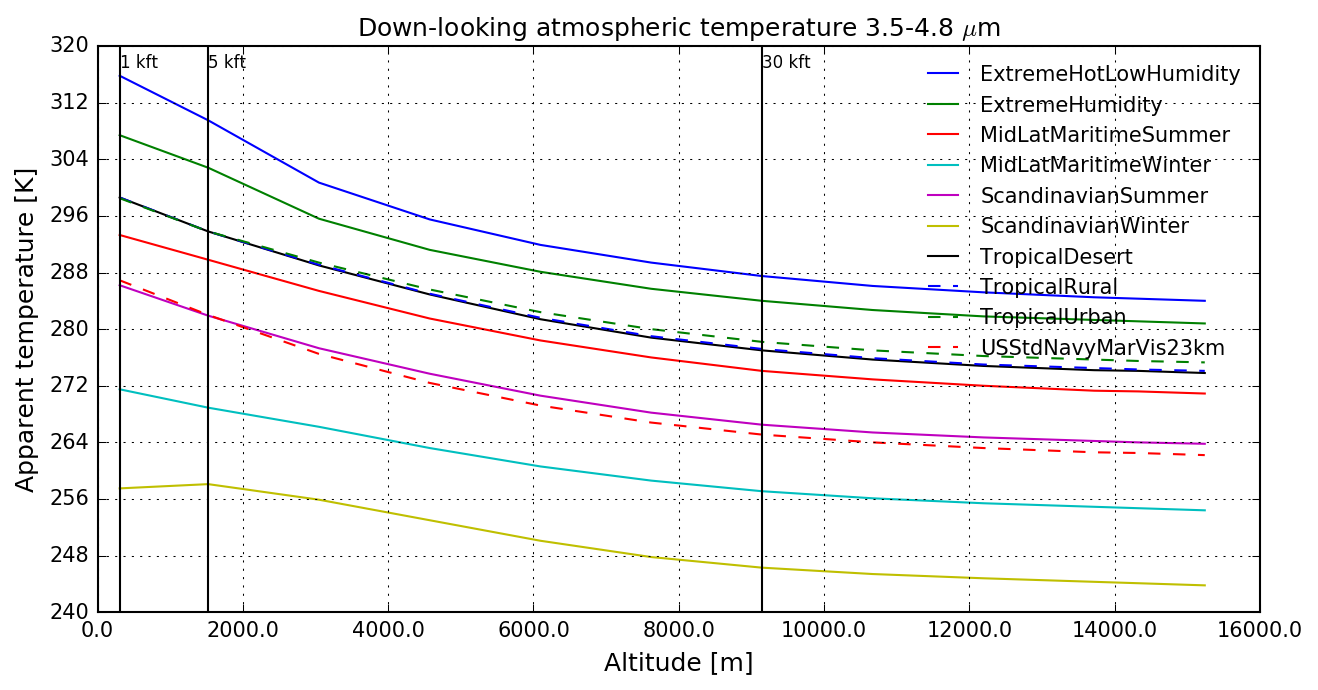
\includegraphics{./pic/Analyse-Standard-Atmospheres_23_0.png}
\end{center}


\section{Effective Transmittance in Spectral Bands}
\label{sec:EffectiveTransmittanceinSpectralBands}

The effective transmittance in a number of spectral bands are calculated next.  The effective transmittance is calculated using 
\begin{equation}\tau_\textrm{eff} = \frac{\int_{\lambda_1}^{\lambda_2} \tau_\lambda\,L_{\lambda\textrm{source}}\,d\lambda}{\int_{\lambda_1}^{\lambda_2} L_{\lambda\textrm{source}}\,d\lambda} = e^{-\gamma R}\end{equation}
where the integration limits are defined by the spectral band, and the source radiance is calculated as a sum of reflected sunlight and emitted thermal radiation at 300 K, 
\begin{equation}L_{\lambda\textrm{source}} = (1\,-\,\rho)\,L_\textrm{planck}(300K) + \xi\,\rho \,L_\textrm{planck}(6000K)\end{equation}
where $\xi=2.1\times10^{-5}$ accounts for the sun's distance and area, $\rho$ is the surface reflection (default value 0.3) and $L_\textrm{planck}$ is Planck law radiance.  The exact value of reflectance is only important in the MWIR spectral band; in other bands the value divides out in the normalisation, and becomes unimportant.


The spectral bands are defined as follows:




See Listing~\ref{lst:autolistingcell25} for the code to define the spectral bands.


\begin{lstlisting}[style=outcellstyle]
{'NIR': [0.7, 0.9], 'Visible': [0.43, 0.69], 'MWIR': [3.6, 4.9], 'LWIR': [8.0, 12.0], 'SWIR': [1.0, 1.7]}
['Visible', 'NIR', 'SWIR', 'MWIR', 'LWIR']

\end{lstlisting}

The function \verb+analyseTau+ calculates the effective transmittance and creates a Pandas dataframe with the results.




See Listing~\ref{lst:autolistingcell27} for the code to calculate effective transmittance.

Calculate the effective transmittance dataframe for the path length as shown below.  The source spectral radiance used in the calculation is also shown below.




See Listing~\ref{lst:autolistingcell29} for the code to define atmospheric conditions.

\begin{center}
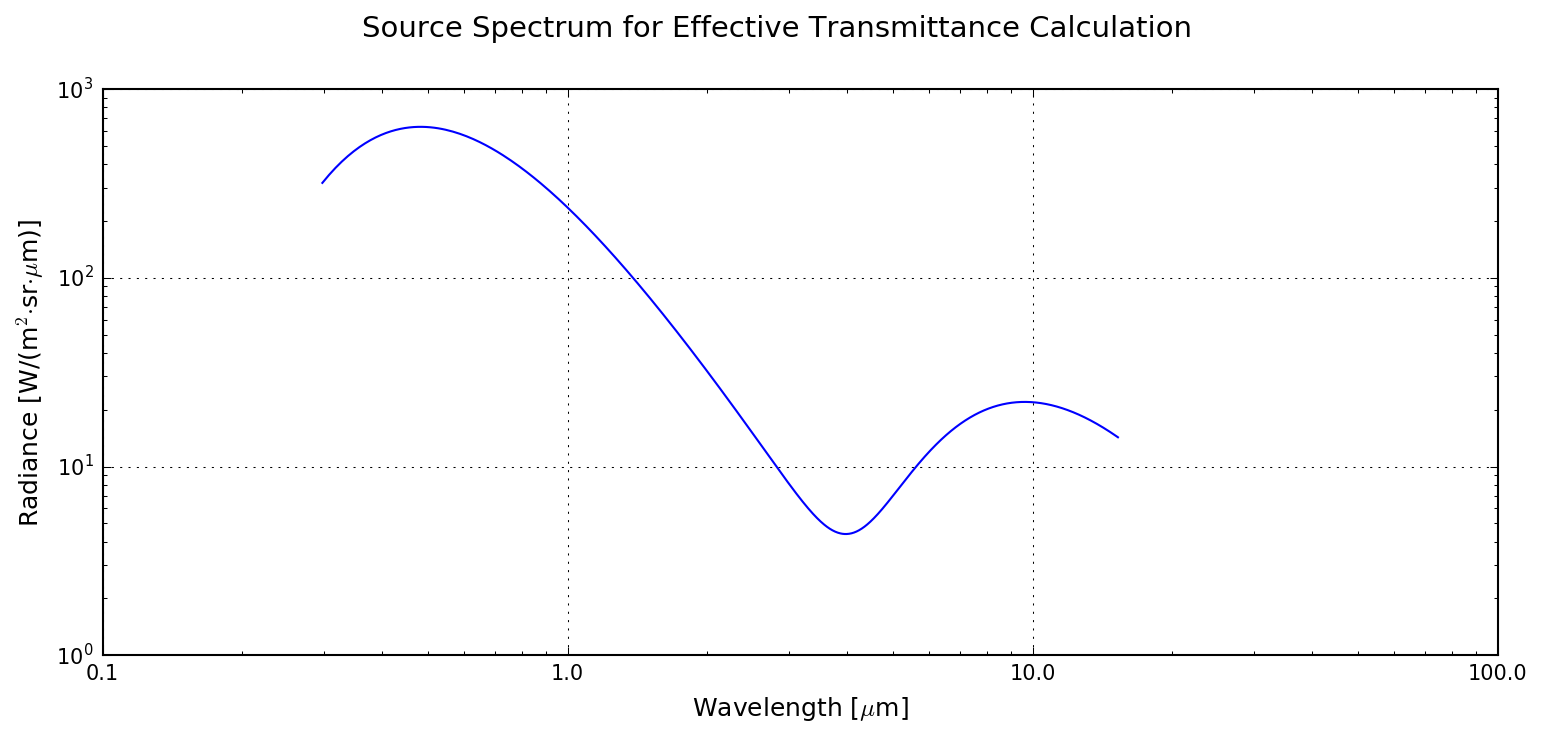
\includegraphics{./pic/Analyse-Standard-Atmospheres_29_0.png}
\end{center}



See Listing~\ref{lst:autolistingcell30} for the code to sort and process the data.

Next manipulate the data to extract and display the effective transmittance values in tabular form for the different altitudes.


The data in the following tables describe two different path types in a somewhat confusing manner. Please note the following:


\begin{enumerate}
\item Slant path from altitude to ground: The first table in the set provides the effective transmittance along the slant path, from the stated altitude to ground, with a slant angle of -45 deg.  The path length quoted here ranges from altitude to ground at a fixed slant angle.
\item Near horizontal path: The second table in the set provides the effective transmittance but scaled to a fixed path length (e.g. 5 km) from the stated altitude, but at some arbitrary slant angle that would give a path length of the stated fixed path length.  In other words the slant angle is adjusted to provide a path length of 5 km. This does not make sense for altitudes above 5 km, but the values are calculated anyway.
\end{enumerate}



See Listing~\ref{lst:autolistingcell32} for the code to build the result tables.




Altitude 305 m, slant path length 431 m, (recalculated from 1 km data set)


\begin{center}

\begin{footnotesize}

\begin{tabular}{|c|c|c|c|c|c|}
\hline
&\multicolumn{5}{|c|}{EffTauSlant}\\\hline
SpecRange&Visible&NIR&SWIR&MWIR&LWIR\\\hline
Atmosphere&&&&&\\\hline
ExtremeHotLowHumidity 44 C, 30\% RH (18.1), 77 km Vis Desert&0.977&0.962&0.783&0.694&0.835\\\hline
ExtremeHumidity 35 C, 95\% RH (37.9), 23 km Vis Rural&0.930&0.914&0.718&0.636&0.585\\\hline
MidLatMaritimeSummer 21 C, 76\% RH (14), 23 km Vis Maritime&0.931&0.923&0.770&0.702&0.865\\\hline
MidLatMaritimeWinter -1 C, 77\% RH (3), 10 km Vis Maritime&0.843&0.855&0.779&0.712&0.946\\\hline
ScandinavianSummer 14 C, 75\% RH (9), 31 km Vis Maritime&0.949&0.943&0.805&0.725&0.910\\\hline
ScandinavianWinter -15.9 C, 80\% RH (1), 31 km Vis Maritime&0.945&0.950&0.892&0.759&0.974\\\hline
TropicalDesert 26.6 C, 75\% RH (18), 75 km Vis Desert&0.976&0.962&0.784&0.702&0.818\\\hline
TropicalRural 26.6 C, 75\% RH (18), 23 km Vis Rural&0.931&0.933&0.770&0.698&0.814\\\hline
TropicalUrban 26.6 C, 75\% RH (18), 5 km Vis Urban&0.714&0.779&0.692&0.673&0.794\\\hline
USStdNavyMarVis23km 15 C, 46\% RH (5.9), 23 km Vis Nav.Mar, SS4&0.932&0.932&0.819&0.738&0.943\\\hline

\end{tabular}
\end{footnotesize}
\end{center}

Altitude 305 m, fixed path length 5000 m, (recalculated from 1 km data set)


\begin{center}

\begin{footnotesize}

\begin{tabular}{|c|c|c|c|c|c|}
\hline
&\multicolumn{5}{|c|}{EffTauRange}\\\hline
SpecRange&Visible&NIR&SWIR&MWIR&LWIR\\\hline
Atmosphere&&&&&\\\hline
ExtremeHotLowHumidity 44 C, 30\% RH (18.1), 77 km Vis Desert&0.764&0.688&0.500&0.252&0.156\\\hline
ExtremeHumidity 35 C, 95\% RH (37.9), 23 km Vis Rural&0.438&0.419&0.351&0.166&0.004\\\hline
MidLatMaritimeSummer 21 C, 76\% RH (14), 23 km Vis Maritime&0.440&0.415&0.316&0.206&0.216\\\hline
MidLatMaritimeWinter -1 C, 77\% RH (3), 10 km Vis Maritime&0.139&0.164&0.149&0.172&0.550\\\hline
ScandinavianSummer 14 C, 75\% RH (9), 31 km Vis Maritime&0.548&0.521&0.385&0.253&0.370\\\hline
ScandinavianWinter -15.9 C, 80\% RH (1), 31 km Vis Maritime&0.522&0.557&0.458&0.352&0.752\\\hline
TropicalDesert 26.6 C, 75\% RH (18), 75 km Vis Desert&0.763&0.689&0.503&0.252&0.122\\\hline
TropicalRural 26.6 C, 75\% RH (18), 23 km Vis Rural&0.444&0.482&0.410&0.236&0.116\\\hline
TropicalUrban 26.6 C, 75\% RH (18), 5 km Vis Urban&0.022&0.061&0.122&0.152&0.086\\\hline
USStdNavyMarVis23km 15 C, 46\% RH (5.9), 23 km Vis Nav.Mar, SS4&0.445&0.455&0.361&0.291&0.541\\\hline

\end{tabular}
\end{footnotesize}
\end{center}



Altitude 1524 m, slant path length 2155 m, (recalculated from 1 km data set)


\begin{center}

\begin{footnotesize}

\begin{tabular}{|c|c|c|c|c|c|}
\hline
&\multicolumn{5}{|c|}{EffTauSlant}\\\hline
SpecRange&Visible&NIR&SWIR&MWIR&LWIR\\\hline
Atmosphere&&&&&\\\hline
ExtremeHotLowHumidity 44 C, 30\% RH (18.1), 77 km Vis Desert&0.911&0.890&0.671&0.497&0.599\\\hline
ExtremeHumidity 35 C, 95\% RH (37.9), 23 km Vis Rural&0.756&0.752&0.569&0.400&0.185\\\hline
MidLatMaritimeSummer 21 C, 76\% RH (14), 23 km Vis Maritime&0.758&0.757&0.594&0.492&0.654\\\hline
MidLatMaritimeWinter -1 C, 77\% RH (3), 10 km Vis Maritime&0.472&0.514&0.469&0.467&0.828\\\hline
ScandinavianSummer 14 C, 75\% RH (9), 31 km Vis Maritime&0.815&0.810&0.642&0.525&0.752\\\hline
ScandinavianWinter -15.9 C, 80\% RH (1), 31 km Vis Maritime&0.802&0.823&0.729&0.581&0.906\\\hline
TropicalDesert 26.6 C, 75\% RH (18), 75 km Vis Desert&0.910&0.889&0.671&0.501&0.540\\\hline
TropicalRural 26.6 C, 75\% RH (18), 23 km Vis Rural&0.759&0.789&0.627&0.491&0.532\\\hline
TropicalUrban 26.6 C, 75\% RH (18), 5 km Vis Urban&0.243&0.363&0.395&0.418&0.475\\\hline
USStdNavyMarVis23km 15 C, 46\% RH (5.9), 23 km Vis Nav.Mar, SS4&0.760&0.772&0.641&0.551&0.835\\\hline

\end{tabular}
\end{footnotesize}
\end{center}

Altitude 1524 m, fixed path length 5000 m, (recalculated from 1 km data set)


\begin{center}

\begin{footnotesize}

\begin{tabular}{|c|c|c|c|c|c|}
\hline
&\multicolumn{5}{|c|}{EffTauRange}\\\hline
SpecRange&Visible&NIR&SWIR&MWIR&LWIR\\\hline
Atmosphere&&&&&\\\hline
ExtremeHotLowHumidity 44 C, 30\% RH (18.1), 77 km Vis Desert&0.806&0.774&0.563&0.329&0.316\\\hline
ExtremeHumidity 35 C, 95\% RH (37.9), 23 km Vis Rural&0.524&0.532&0.426&0.233&0.026\\\hline
MidLatMaritimeSummer 21 C, 76\% RH (14), 23 km Vis Maritime&0.527&0.529&0.408&0.302&0.382\\\hline
MidLatMaritimeWinter -1 C, 77\% RH (3), 10 km Vis Maritime&0.176&0.214&0.206&0.251&0.651\\\hline
ScandinavianSummer 14 C, 75\% RH (9), 31 km Vis Maritime&0.623&0.617&0.465&0.339&0.524\\\hline
ScandinavianWinter -15.9 C, 80\% RH (1), 31 km Vis Maritime&0.601&0.638&0.539&0.417&0.799\\\hline
TropicalDesert 26.6 C, 75\% RH (18), 75 km Vis Desert&0.804&0.772&0.564&0.330&0.251\\\hline
TropicalRural 26.6 C, 75\% RH (18), 23 km Vis Rural&0.530&0.586&0.482&0.314&0.242\\\hline
TropicalUrban 26.6 C, 75\% RH (18), 5 km Vis Urban&0.039&0.098&0.167&0.215&0.185\\\hline
USStdNavyMarVis23km 15 C, 46\% RH (5.9), 23 km Vis Nav.Mar, SS4&0.530&0.552&0.444&0.375&0.665\\\hline

\end{tabular}
\end{footnotesize}
\end{center}



Altitude 3048 m, slant path length 4311 m, (recalculated from 1 km data set)


\begin{center}

\begin{footnotesize}

\begin{tabular}{|c|c|c|c|c|c|}
\hline
&\multicolumn{5}{|c|}{EffTauSlant}\\\hline
SpecRange&Visible&NIR&SWIR&MWIR&LWIR\\\hline
Atmosphere&&&&&\\\hline
ExtremeHotLowHumidity 44 C, 30\% RH (18.1), 77 km Vis Desert&0.863&0.857&0.644&0.441&0.548\\\hline
ExtremeHumidity 35 C, 95\% RH (37.9), 23 km Vis Rural&0.656&0.677&0.526&0.341&0.133\\\hline
MidLatMaritimeSummer 21 C, 76\% RH (14), 23 km Vis Maritime&0.658&0.674&0.530&0.419&0.578\\\hline
MidLatMaritimeWinter -1 C, 77\% RH (3), 10 km Vis Maritime&0.404&0.456&0.416&0.407&0.789\\\hline
ScandinavianSummer 14 C, 75\% RH (9), 31 km Vis Maritime&0.732&0.739&0.580&0.449&0.681\\\hline
ScandinavianWinter -15.9 C, 80\% RH (1), 31 km Vis Maritime&0.718&0.755&0.660&0.509&0.867\\\hline
TropicalDesert 26.6 C, 75\% RH (18), 75 km Vis Desert&0.861&0.850&0.634&0.432&0.443\\\hline
TropicalRural 26.6 C, 75\% RH (18), 23 km Vis Rural&0.659&0.713&0.574&0.419&0.433\\\hline
TropicalUrban 26.6 C, 75\% RH (18), 5 km Vis Urban&0.204&0.320&0.356&0.354&0.385\\\hline
USStdNavyMarVis23km 15 C, 46\% RH (5.9), 23 km Vis Nav.Mar, SS4&0.660&0.689&0.570&0.478&0.781\\\hline

\end{tabular}
\end{footnotesize}
\end{center}

Altitude 3048 m, fixed path length 5000 m, (recalculated from 1 km data set)


\begin{center}

\begin{footnotesize}

\begin{tabular}{|c|c|c|c|c|c|}
\hline
&\multicolumn{5}{|c|}{EffTauRange}\\\hline
SpecRange&Visible&NIR&SWIR&MWIR&LWIR\\\hline
Atmosphere&&&&&\\\hline
ExtremeHotLowHumidity 44 C, 30\% RH (18.1), 77 km Vis Desert&0.843&0.838&0.625&0.411&0.500\\\hline
ExtremeHumidity 35 C, 95\% RH (37.9), 23 km Vis Rural&0.613&0.638&0.500&0.310&0.098\\\hline
MidLatMaritimeSummer 21 C, 76\% RH (14), 23 km Vis Maritime&0.615&0.633&0.497&0.385&0.531\\\hline
MidLatMaritimeWinter -1 C, 77\% RH (3), 10 km Vis Maritime&0.350&0.402&0.369&0.370&0.760\\\hline
ScandinavianSummer 14 C, 75\% RH (9), 31 km Vis Maritime&0.696&0.705&0.548&0.416&0.641\\\hline
ScandinavianWinter -15.9 C, 80\% RH (1), 31 km Vis Maritime&0.681&0.722&0.626&0.480&0.847\\\hline
TropicalDesert 26.6 C, 75\% RH (18), 75 km Vis Desert&0.841&0.829&0.614&0.401&0.390\\\hline
TropicalRural 26.6 C, 75\% RH (18), 23 km Vis Rural&0.617&0.677&0.548&0.387&0.381\\\hline
TropicalUrban 26.6 C, 75\% RH (18), 5 km Vis Urban&0.159&0.267&0.315&0.318&0.332\\\hline
USStdNavyMarVis23km 15 C, 46\% RH (5.9), 23 km Vis Nav.Mar, SS4&0.618&0.650&0.535&0.447&0.752\\\hline

\end{tabular}
\end{footnotesize}
\end{center}



Altitude 4572 m, slant path length 6466 m, (recalculated from 1 km data set)


\begin{center}

\begin{footnotesize}

\begin{tabular}{|c|c|c|c|c|c|}
\hline
&\multicolumn{5}{|c|}{EffTauSlant}\\\hline
SpecRange&Visible&NIR&SWIR&MWIR&LWIR\\\hline
Atmosphere&&&&&\\\hline
ExtremeHotLowHumidity 44 C, 30\% RH (18.1), 77 km Vis Desert&0.830&0.840&0.634&0.416&0.533\\\hline
ExtremeHumidity 35 C, 95\% RH (37.9), 23 km Vis Rural&0.613&0.652&0.513&0.320&0.125\\\hline
MidLatMaritimeSummer 21 C, 76\% RH (14), 23 km Vis Maritime&0.615&0.648&0.516&0.393&0.557\\\hline
MidLatMaritimeWinter -1 C, 77\% RH (3), 10 km Vis Maritime&0.384&0.443&0.407&0.385&0.775\\\hline
ScandinavianSummer 14 C, 75\% RH (9), 31 km Vis Maritime&0.692&0.716&0.564&0.422&0.658\\\hline
ScandinavianWinter -15.9 C, 80\% RH (1), 31 km Vis Maritime&0.685&0.738&0.646&0.484&0.854\\\hline
TropicalDesert 26.6 C, 75\% RH (18), 75 km Vis Desert&0.829&0.831&0.622&0.405&0.424\\\hline
TropicalRural 26.6 C, 75\% RH (18), 23 km Vis Rural&0.617&0.686&0.559&0.393&0.414\\\hline
TropicalUrban 26.6 C, 75\% RH (18), 5 km Vis Urban&0.192&0.308&0.346&0.332&0.368\\\hline
USStdNavyMarVis23km 15 C, 46\% RH (5.9), 23 km Vis Nav.Mar, SS4&0.617&0.664&0.555&0.451&0.763\\\hline

\end{tabular}
\end{footnotesize}
\end{center}

Altitude 4572 m, fixed path length 5000 m, (recalculated from 1 km data set)


\begin{center}

\begin{footnotesize}

\begin{tabular}{|c|c|c|c|c|c|}
\hline
&\multicolumn{5}{|c|}{EffTauRange}\\\hline
SpecRange&Visible&NIR&SWIR&MWIR&LWIR\\\hline
Atmosphere&&&&&\\\hline
ExtremeHotLowHumidity 44 C, 30\% RH (18.1), 77 km Vis Desert&0.866&0.873&0.668&0.468&0.612\\\hline
ExtremeHumidity 35 C, 95\% RH (37.9), 23 km Vis Rural&0.685&0.716&0.557&0.374&0.195\\\hline
MidLatMaritimeSummer 21 C, 76\% RH (14), 23 km Vis Maritime&0.687&0.714&0.572&0.450&0.634\\\hline
MidLatMaritimeWinter -1 C, 77\% RH (3), 10 km Vis Maritime&0.476&0.533&0.485&0.446&0.820\\\hline
ScandinavianSummer 14 C, 75\% RH (9), 31 km Vis Maritime&0.752&0.772&0.617&0.477&0.722\\\hline
ScandinavianWinter -15.9 C, 80\% RH (1), 31 km Vis Maritime&0.746&0.790&0.700&0.532&0.885\\\hline
TropicalDesert 26.6 C, 75\% RH (18), 75 km Vis Desert&0.864&0.865&0.655&0.458&0.512\\\hline
TropicalRural 26.6 C, 75\% RH (18), 23 km Vis Rural&0.688&0.746&0.604&0.448&0.503\\\hline
TropicalUrban 26.6 C, 75\% RH (18), 5 km Vis Urban&0.278&0.401&0.417&0.393&0.459\\\hline
USStdNavyMarVis23km 15 C, 46\% RH (5.9), 23 km Vis Nav.Mar, SS4&0.689&0.728&0.613&0.503&0.810\\\hline

\end{tabular}
\end{footnotesize}
\end{center}



Altitude 6096 m, slant path length 8621 m, (recalculated from 1 km data set)


\begin{center}

\begin{footnotesize}

\begin{tabular}{|c|c|c|c|c|c|}
\hline
&\multicolumn{5}{|c|}{EffTauSlant}\\\hline
SpecRange&Visible&NIR&SWIR&MWIR&LWIR\\\hline
Atmosphere&&&&&\\\hline
ExtremeHotLowHumidity 44 C, 30\% RH (18.1), 77 km Vis Desert&0.801&0.826&0.627&0.401&0.524\\\hline
ExtremeHumidity 35 C, 95\% RH (37.9), 23 km Vis Rural&0.591&0.640&0.508&0.309&0.122\\\hline
MidLatMaritimeSummer 21 C, 76\% RH (14), 23 km Vis Maritime&0.593&0.637&0.510&0.379&0.547\\\hline
MidLatMaritimeWinter -1 C, 77\% RH (3), 10 km Vis Maritime&0.373&0.438&0.403&0.372&0.766\\\hline
ScandinavianSummer 14 C, 75\% RH (9), 31 km Vis Maritime&0.667&0.703&0.557&0.407&0.647\\\hline
ScandinavianWinter -15.9 C, 80\% RH (1), 31 km Vis Maritime&0.667&0.730&0.640&0.469&0.847\\\hline
TropicalDesert 26.6 C, 75\% RH (18), 75 km Vis Desert&0.800&0.816&0.614&0.390&0.416\\\hline
TropicalRural 26.6 C, 75\% RH (18), 23 km Vis Rural&0.595&0.674&0.552&0.379&0.407\\\hline
TropicalUrban 26.6 C, 75\% RH (18), 5 km Vis Urban&0.185&0.303&0.342&0.320&0.361\\\hline
USStdNavyMarVis23km 15 C, 46\% RH (5.9), 23 km Vis Nav.Mar, SS4&0.595&0.653&0.548&0.436&0.754\\\hline

\end{tabular}
\end{footnotesize}
\end{center}

Altitude 6096 m, fixed path length 5000 m, (recalculated from 1 km data set)


\begin{center}

\begin{footnotesize}

\begin{tabular}{|c|c|c|c|c|c|}
\hline
&\multicolumn{5}{|c|}{EffTauRange}\\\hline
SpecRange&Visible&NIR&SWIR&MWIR&LWIR\\\hline
Atmosphere&&&&&\\\hline
ExtremeHotLowHumidity 44 C, 30\% RH (18.1), 77 km Vis Desert&0.879&0.893&0.700&0.509&0.684\\\hline
ExtremeHumidity 35 C, 95\% RH (37.9), 23 km Vis Rural&0.737&0.768&0.599&0.424&0.284\\\hline
MidLatMaritimeSummer 21 C, 76\% RH (14), 23 km Vis Maritime&0.738&0.768&0.625&0.497&0.702\\\hline
MidLatMaritimeWinter -1 C, 77\% RH (3), 10 km Vis Maritime&0.564&0.619&0.564&0.496&0.855\\\hline
ScandinavianSummer 14 C, 75\% RH (9), 31 km Vis Maritime&0.790&0.814&0.665&0.520&0.775\\\hline
ScandinavianWinter -15.9 C, 80\% RH (1), 31 km Vis Maritime&0.790&0.833&0.749&0.567&0.907\\\hline
TropicalDesert 26.6 C, 75\% RH (18), 75 km Vis Desert&0.878&0.887&0.687&0.500&0.596\\\hline
TropicalRural 26.6 C, 75\% RH (18), 23 km Vis Rural&0.739&0.793&0.646&0.492&0.589\\\hline
TropicalUrban 26.6 C, 75\% RH (18), 5 km Vis Urban&0.374&0.498&0.489&0.446&0.550\\\hline
USStdNavyMarVis23km 15 C, 46\% RH (5.9), 23 km Vis Nav.Mar, SS4&0.740&0.780&0.666&0.542&0.847\\\hline

\end{tabular}
\end{footnotesize}
\end{center}



Altitude 7620 m, slant path length 10776 m, (recalculated from 1 km data set)


\begin{center}

\begin{footnotesize}

\begin{tabular}{|c|c|c|c|c|c|}
\hline
&\multicolumn{5}{|c|}{EffTauSlant}\\\hline
SpecRange&Visible&NIR&SWIR&MWIR&LWIR\\\hline
Atmosphere&&&&&\\\hline
ExtremeHotLowHumidity 44 C, 30\% RH (18.1), 77 km Vis Desert&0.779&0.816&0.622&0.392&0.517\\\hline
ExtremeHumidity 35 C, 95\% RH (37.9), 23 km Vis Rural&0.575&0.633&0.505&0.302&0.120\\\hline
MidLatMaritimeSummer 21 C, 76\% RH (14), 23 km Vis Maritime&0.577&0.629&0.506&0.371&0.540\\\hline
MidLatMaritimeWinter -1 C, 77\% RH (3), 10 km Vis Maritime&0.366&0.435&0.401&0.364&0.759\\\hline
ScandinavianSummer 14 C, 75\% RH (9), 31 km Vis Maritime&0.649&0.695&0.553&0.398&0.640\\\hline
ScandinavianWinter -15.9 C, 80\% RH (1), 31 km Vis Maritime&0.654&0.725&0.637&0.459&0.839\\\hline
TropicalDesert 26.6 C, 75\% RH (18), 75 km Vis Desert&0.778&0.807&0.610&0.381&0.411\\\hline
TropicalRural 26.6 C, 75\% RH (18), 23 km Vis Rural&0.579&0.666&0.549&0.370&0.402\\\hline
TropicalUrban 26.6 C, 75\% RH (18), 5 km Vis Urban&0.180&0.299&0.340&0.312&0.357\\\hline
USStdNavyMarVis23km 15 C, 46\% RH (5.9), 23 km Vis Nav.Mar, SS4&0.579&0.645&0.544&0.426&0.748\\\hline

\end{tabular}
\end{footnotesize}
\end{center}

Altitude 7620 m, fixed path length 5000 m, (recalculated from 1 km data set)


\begin{center}

\begin{footnotesize}

\begin{tabular}{|c|c|c|c|c|c|}
\hline
&\multicolumn{5}{|c|}{EffTauRange}\\\hline
SpecRange&Visible&NIR&SWIR&MWIR&LWIR\\\hline
Atmosphere&&&&&\\\hline
ExtremeHotLowHumidity 44 C, 30\% RH (18.1), 77 km Vis Desert&0.890&0.908&0.725&0.541&0.732\\\hline
ExtremeHumidity 35 C, 95\% RH (37.9), 23 km Vis Rural&0.773&0.805&0.632&0.463&0.359\\\hline
MidLatMaritimeSummer 21 C, 76\% RH (14), 23 km Vis Maritime&0.774&0.805&0.663&0.532&0.748\\\hline
MidLatMaritimeWinter -1 C, 77\% RH (3), 10 km Vis Maritime&0.626&0.679&0.621&0.533&0.878\\\hline
ScandinavianSummer 14 C, 75\% RH (9), 31 km Vis Maritime&0.818&0.844&0.701&0.553&0.810\\\hline
ScandinavianWinter -15.9 C, 80\% RH (1), 31 km Vis Maritime&0.820&0.861&0.785&0.594&0.921\\\hline
TropicalDesert 26.6 C, 75\% RH (18), 75 km Vis Desert&0.889&0.903&0.712&0.534&0.657\\\hline
TropicalRural 26.6 C, 75\% RH (18), 23 km Vis Rural&0.775&0.826&0.678&0.526&0.650\\\hline
TropicalUrban 26.6 C, 75\% RH (18), 5 km Vis Urban&0.448&0.569&0.542&0.487&0.616\\\hline
USStdNavyMarVis23km 15 C, 46\% RH (5.9), 23 km Vis Nav.Mar, SS4&0.775&0.815&0.705&0.572&0.872\\\hline

\end{tabular}
\end{footnotesize}
\end{center}



Altitude 9144 m, slant path length 12932 m, (recalculated from 1 km data set)


\begin{center}

\begin{footnotesize}

\begin{tabular}{|c|c|c|c|c|c|}
\hline
&\multicolumn{5}{|c|}{EffTauSlant}\\\hline
SpecRange&Visible&NIR&SWIR&MWIR&LWIR\\\hline
Atmosphere&&&&&\\\hline
ExtremeHotLowHumidity 44 C, 30\% RH (18.1), 77 km Vis Desert&0.765&0.811&0.620&0.386&0.512\\\hline
ExtremeHumidity 35 C, 95\% RH (37.9), 23 km Vis Rural&0.565&0.628&0.503&0.297&0.118\\\hline
MidLatMaritimeSummer 21 C, 76\% RH (14), 23 km Vis Maritime&0.567&0.625&0.504&0.365&0.535\\\hline
MidLatMaritimeWinter -1 C, 77\% RH (3), 10 km Vis Maritime&0.361&0.433&0.400&0.359&0.751\\\hline
ScandinavianSummer 14 C, 75\% RH (9), 31 km Vis Maritime&0.638&0.691&0.551&0.392&0.633\\\hline
ScandinavianWinter -15.9 C, 80\% RH (1), 31 km Vis Maritime&0.644&0.722&0.636&0.453&0.830\\\hline
TropicalDesert 26.6 C, 75\% RH (18), 75 km Vis Desert&0.764&0.801&0.608&0.375&0.408\\\hline
TropicalRural 26.6 C, 75\% RH (18), 23 km Vis Rural&0.569&0.661&0.547&0.364&0.399\\\hline
TropicalUrban 26.6 C, 75\% RH (18), 5 km Vis Urban&0.177&0.297&0.339&0.307&0.355\\\hline
USStdNavyMarVis23km 15 C, 46\% RH (5.9), 23 km Vis Nav.Mar, SS4&0.569&0.641&0.542&0.419&0.743\\\hline

\end{tabular}
\end{footnotesize}
\end{center}

Altitude 9144 m, fixed path length 5000 m, (recalculated from 1 km data set)


\begin{center}

\begin{footnotesize}

\begin{tabular}{|c|c|c|c|c|c|}
\hline
&\multicolumn{5}{|c|}{EffTauRange}\\\hline
SpecRange&Visible&NIR&SWIR&MWIR&LWIR\\\hline
Atmosphere&&&&&\\\hline
ExtremeHotLowHumidity 44 C, 30\% RH (18.1), 77 km Vis Desert&0.901&0.920&0.746&0.566&0.767\\\hline
ExtremeHumidity 35 C, 95\% RH (37.9), 23 km Vis Rural&0.801&0.832&0.658&0.495&0.422\\\hline
MidLatMaritimeSummer 21 C, 76\% RH (14), 23 km Vis Maritime&0.802&0.832&0.694&0.560&0.782\\\hline
MidLatMaritimeWinter -1 C, 77\% RH (3), 10 km Vis Maritime&0.673&0.723&0.664&0.562&0.893\\\hline
ScandinavianSummer 14 C, 75\% RH (9), 31 km Vis Maritime&0.839&0.865&0.729&0.579&0.835\\\hline
ScandinavianWinter -15.9 C, 80\% RH (1), 31 km Vis Maritime&0.843&0.881&0.811&0.615&0.929\\\hline
TropicalDesert 26.6 C, 75\% RH (18), 75 km Vis Desert&0.900&0.915&0.733&0.561&0.702\\\hline
TropicalRural 26.6 C, 75\% RH (18), 23 km Vis Rural&0.803&0.850&0.704&0.554&0.696\\\hline
TropicalUrban 26.6 C, 75\% RH (18), 5 km Vis Urban&0.509&0.623&0.584&0.520&0.665\\\hline
USStdNavyMarVis23km 15 C, 46\% RH (5.9), 23 km Vis Nav.Mar, SS4&0.803&0.841&0.735&0.595&0.889\\\hline

\end{tabular}
\end{footnotesize}
\end{center}


Altitude 10668 m, slant path length 15087 m, (recalculated from 1 km data set)


\begin{center}

\begin{footnotesize}

\begin{tabular}{|c|c|c|c|c|c|}
\hline
&\multicolumn{5}{|c|}{EffTauSlant}\\\hline
SpecRange&Visible&NIR&SWIR&MWIR&LWIR\\\hline
Atmosphere&&&&&\\\hline
ExtremeHotLowHumidity 44 C, 30\% RH (18.1), 77 km Vis Desert&0.755&0.807&0.619&0.381&0.507\\\hline
ExtremeHumidity 35 C, 95\% RH (37.9), 23 km Vis Rural&0.558&0.626&0.502&0.293&0.117\\\hline
MidLatMaritimeSummer 21 C, 76\% RH (14), 23 km Vis Maritime&0.560&0.622&0.503&0.360&0.530\\\hline
MidLatMaritimeWinter -1 C, 77\% RH (3), 10 km Vis Maritime&0.356&0.432&0.399&0.355&0.741\\\hline
ScandinavianSummer 14 C, 75\% RH (9), 31 km Vis Maritime&0.629&0.688&0.550&0.388&0.626\\\hline
ScandinavianWinter -15.9 C, 80\% RH (1), 31 km Vis Maritime&0.637&0.719&0.635&0.448&0.818\\\hline
TropicalDesert 26.6 C, 75\% RH (18), 75 km Vis Desert&0.755&0.798&0.607&0.371&0.406\\\hline
TropicalRural 26.6 C, 75\% RH (18), 23 km Vis Rural&0.562&0.658&0.545&0.360&0.397\\\hline
TropicalUrban 26.6 C, 75\% RH (18), 5 km Vis Urban&0.175&0.296&0.338&0.304&0.353\\\hline
USStdNavyMarVis23km 15 C, 46\% RH (5.9), 23 km Vis Nav.Mar, SS4&0.562&0.638&0.541&0.415&0.736\\\hline

\end{tabular}
\end{footnotesize}
\end{center}

Altitude 10668 m, fixed path length 5000 m, (recalculated from 1 km data set)


\begin{center}

\begin{footnotesize}

\begin{tabular}{|c|c|c|c|c|c|}
\hline
&\multicolumn{5}{|c|}{EffTauRange}\\\hline
SpecRange&Visible&NIR&SWIR&MWIR&LWIR\\\hline
Atmosphere&&&&&\\\hline
ExtremeHotLowHumidity 44 C, 30\% RH (18.1), 77 km Vis Desert&0.910&0.930&0.763&0.588&0.794\\\hline
ExtremeHumidity 35 C, 95\% RH (37.9), 23 km Vis Rural&0.823&0.852&0.680&0.522&0.474\\\hline
MidLatMaritimeSummer 21 C, 76\% RH (14), 23 km Vis Maritime&0.824&0.853&0.718&0.582&0.807\\\hline
MidLatMaritimeWinter -1 C, 77\% RH (3), 10 km Vis Maritime&0.709&0.756&0.698&0.585&0.903\\\hline
ScandinavianSummer 14 C, 75\% RH (9), 31 km Vis Maritime&0.857&0.882&0.752&0.601&0.853\\\hline
ScandinavianWinter -15.9 C, 80\% RH (1), 31 km Vis Maritime&0.860&0.896&0.832&0.633&0.934\\\hline
TropicalDesert 26.6 C, 75\% RH (18), 75 km Vis Desert&0.910&0.926&0.751&0.583&0.736\\\hline
TropicalRural 26.6 C, 75\% RH (18), 23 km Vis Rural&0.825&0.868&0.725&0.577&0.731\\\hline
TropicalUrban 26.6 C, 75\% RH (18), 5 km Vis Urban&0.557&0.665&0.618&0.546&0.703\\\hline
USStdNavyMarVis23km 15 C, 46\% RH (5.9), 23 km Vis Nav.Mar, SS4&0.825&0.861&0.759&0.615&0.901\\\hline

\end{tabular}
\end{footnotesize}
\end{center}


Altitude 12192 m, slant path length 17242 m, (recalculated from 1 km data set)


\begin{center}

\begin{footnotesize}

\begin{tabular}{|c|c|c|c|c|c|}
\hline
&\multicolumn{5}{|c|}{EffTauSlant}\\\hline
SpecRange&Visible&NIR&SWIR&MWIR&LWIR\\\hline
Atmosphere&&&&&\\\hline
ExtremeHotLowHumidity 44 C, 30\% RH (18.1), 77 km Vis Desert&0.747&0.805&0.618&0.378&0.501\\\hline
ExtremeHumidity 35 C, 95\% RH (37.9), 23 km Vis Rural&0.552&0.624&0.501&0.291&0.115\\\hline
MidLatMaritimeSummer 21 C, 76\% RH (14), 23 km Vis Maritime&0.554&0.621&0.503&0.357&0.524\\\hline
MidLatMaritimeWinter -1 C, 77\% RH (3), 10 km Vis Maritime&0.352&0.430&0.399&0.352&0.729\\\hline
ScandinavianSummer 14 C, 75\% RH (9), 31 km Vis Maritime&0.623&0.686&0.549&0.385&0.617\\\hline
ScandinavianWinter -15.9 C, 80\% RH (1), 31 km Vis Maritime&0.630&0.718&0.634&0.444&0.807\\\hline
TropicalDesert 26.6 C, 75\% RH (18), 75 km Vis Desert&0.747&0.796&0.606&0.368&0.404\\\hline
TropicalRural 26.6 C, 75\% RH (18), 23 km Vis Rural&0.556&0.657&0.545&0.357&0.395\\\hline
TropicalUrban 26.6 C, 75\% RH (18), 5 km Vis Urban&0.174&0.295&0.337&0.301&0.351\\\hline
USStdNavyMarVis23km 15 C, 46\% RH (5.9), 23 km Vis Nav.Mar, SS4&0.556&0.636&0.540&0.411&0.727\\\hline

\end{tabular}
\end{footnotesize}
\end{center}

Altitude 12192 m, fixed path length 5000 m, (recalculated from 1 km data set)


\begin{center}

\begin{footnotesize}

\begin{tabular}{|c|c|c|c|c|c|}
\hline
&\multicolumn{5}{|c|}{EffTauRange}\\\hline
SpecRange&Visible&NIR&SWIR&MWIR&LWIR\\\hline
Atmosphere&&&&&\\\hline
ExtremeHotLowHumidity 44 C, 30\% RH (18.1), 77 km Vis Desert&0.918&0.937&0.778&0.606&0.814\\\hline
ExtremeHumidity 35 C, 95\% RH (37.9), 23 km Vis Rural&0.840&0.868&0.698&0.545&0.517\\\hline
MidLatMaritimeSummer 21 C, 76\% RH (14), 23 km Vis Maritime&0.841&0.869&0.738&0.602&0.826\\\hline
MidLatMaritimeWinter -1 C, 77\% RH (3), 10 km Vis Maritime&0.738&0.782&0.726&0.605&0.910\\\hline
ScandinavianSummer 14 C, 75\% RH (9), 31 km Vis Maritime&0.871&0.895&0.770&0.618&0.866\\\hline
ScandinavianWinter -15.9 C, 80\% RH (1), 31 km Vis Maritime&0.874&0.908&0.848&0.648&0.937\\\hline
TropicalDesert 26.6 C, 75\% RH (18), 75 km Vis Desert&0.918&0.934&0.766&0.602&0.764\\\hline
TropicalRural 26.6 C, 75\% RH (18), 23 km Vis Rural&0.842&0.883&0.742&0.597&0.759\\\hline
TropicalUrban 26.6 C, 75\% RH (18), 5 km Vis Urban&0.598&0.699&0.646&0.568&0.733\\\hline
USStdNavyMarVis23km 15 C, 46\% RH (5.9), 23 km Vis Nav.Mar, SS4&0.842&0.876&0.778&0.631&0.909\\\hline

\end{tabular}
\end{footnotesize}
\end{center}


Altitude 13716 m, slant path length 19397 m, (recalculated from 1 km data set)


\begin{center}

\begin{footnotesize}

\begin{tabular}{|c|c|c|c|c|c|}
\hline
&\multicolumn{5}{|c|}{EffTauSlant}\\\hline
SpecRange&Visible&NIR&SWIR&MWIR&LWIR\\\hline
Atmosphere&&&&&\\\hline
ExtremeHotLowHumidity 44 C, 30\% RH (18.1), 77 km Vis Desert&0.741&0.803&0.617&0.375&0.495\\\hline
ExtremeHumidity 35 C, 95\% RH (37.9), 23 km Vis Rural&0.547&0.623&0.501&0.289&0.113\\\hline
MidLatMaritimeSummer 21 C, 76\% RH (14), 23 km Vis Maritime&0.549&0.619&0.502&0.355&0.518\\\hline
MidLatMaritimeWinter -1 C, 77\% RH (3), 10 km Vis Maritime&0.349&0.429&0.398&0.349&0.718\\\hline
ScandinavianSummer 14 C, 75\% RH (9), 31 km Vis Maritime&0.617&0.684&0.549&0.382&0.608\\\hline
ScandinavianWinter -15.9 C, 80\% RH (1), 31 km Vis Maritime&0.625&0.716&0.634&0.441&0.796\\\hline
TropicalDesert 26.6 C, 75\% RH (18), 75 km Vis Desert&0.741&0.794&0.605&0.366&0.402\\\hline
TropicalRural 26.6 C, 75\% RH (18), 23 km Vis Rural&0.552&0.655&0.544&0.355&0.393\\\hline
TropicalUrban 26.6 C, 75\% RH (18), 5 km Vis Urban&0.172&0.294&0.337&0.299&0.349\\\hline
USStdNavyMarVis23km 15 C, 46\% RH (5.9), 23 km Vis Nav.Mar, SS4&0.551&0.635&0.539&0.409&0.718\\\hline

\end{tabular}
\end{footnotesize}
\end{center}

Altitude 13716 m, fixed path length 5000 m, (recalculated from 1 km data set)


\begin{center}

\begin{footnotesize}

\begin{tabular}{|c|c|c|c|c|c|}
\hline
&\multicolumn{5}{|c|}{EffTauRange}\\\hline
SpecRange&Visible&NIR&SWIR&MWIR&LWIR\\\hline
Atmosphere&&&&&\\\hline
ExtremeHotLowHumidity 44 C, 30\% RH (18.1), 77 km Vis Desert&0.925&0.943&0.790&0.621&0.830\\\hline
ExtremeHumidity 35 C, 95\% RH (37.9), 23 km Vis Rural&0.854&0.881&0.714&0.565&0.553\\\hline
MidLatMaritimeSummer 21 C, 76\% RH (14), 23 km Vis Maritime&0.856&0.882&0.755&0.618&0.841\\\hline
MidLatMaritimeWinter -1 C, 77\% RH (3), 10 km Vis Maritime&0.761&0.803&0.748&0.621&0.915\\\hline
ScandinavianSummer 14 C, 75\% RH (9), 31 km Vis Maritime&0.882&0.906&0.786&0.634&0.876\\\hline
ScandinavianWinter -15.9 C, 80\% RH (1), 31 km Vis Maritime&0.885&0.917&0.862&0.661&0.940\\\hline
TropicalDesert 26.6 C, 75\% RH (18), 75 km Vis Desert&0.925&0.940&0.778&0.618&0.785\\\hline
TropicalRural 26.6 C, 75\% RH (18), 23 km Vis Rural&0.856&0.895&0.757&0.613&0.781\\\hline
TropicalUrban 26.6 C, 75\% RH (18), 5 km Vis Urban&0.631&0.727&0.669&0.587&0.758\\\hline
USStdNavyMarVis23km 15 C, 46\% RH (5.9), 23 km Vis Nav.Mar, SS4&0.857&0.889&0.795&0.645&0.916\\\hline

\end{tabular}
\end{footnotesize}
\end{center}



Altitude 14326 m, slant path length 20260 m, (recalculated from 1 km data set)


\begin{center}

\begin{footnotesize}

\begin{tabular}{|c|c|c|c|c|c|}
\hline
&\multicolumn{5}{|c|}{EffTauSlant}\\\hline
SpecRange&Visible&NIR&SWIR&MWIR&LWIR\\\hline
Atmosphere&&&&&\\\hline
ExtremeHotLowHumidity 44 C, 30\% RH (18.1), 77 km Vis Desert&0.738&0.803&0.617&0.374&0.493\\\hline
ExtremeHumidity 35 C, 95\% RH (37.9), 23 km Vis Rural&0.545&0.622&0.501&0.288&0.112\\\hline
MidLatMaritimeSummer 21 C, 76\% RH (14), 23 km Vis Maritime&0.547&0.619&0.502&0.354&0.516\\\hline
MidLatMaritimeWinter -1 C, 77\% RH (3), 10 km Vis Maritime&0.348&0.429&0.398&0.348&0.714\\\hline
ScandinavianSummer 14 C, 75\% RH (9), 31 km Vis Maritime&0.615&0.684&0.549&0.381&0.605\\\hline
ScandinavianWinter -15.9 C, 80\% RH (1), 31 km Vis Maritime&0.623&0.715&0.633&0.440&0.791\\\hline
TropicalDesert 26.6 C, 75\% RH (18), 75 km Vis Desert&0.739&0.793&0.605&0.365&0.401\\\hline
TropicalRural 26.6 C, 75\% RH (18), 23 km Vis Rural&0.550&0.655&0.544&0.354&0.392\\\hline
TropicalUrban 26.6 C, 75\% RH (18), 5 km Vis Urban&0.172&0.294&0.337&0.299&0.348\\\hline
USStdNavyMarVis23km 15 C, 46\% RH (5.9), 23 km Vis Nav.Mar, SS4&0.549&0.634&0.539&0.408&0.715\\\hline

\end{tabular}
\end{footnotesize}
\end{center}

Altitude 14326 m, fixed path length 5000 m, (recalculated from 1 km data set)


\begin{center}

\begin{footnotesize}

\begin{tabular}{|c|c|c|c|c|c|}
\hline
&\multicolumn{5}{|c|}{EffTauRange}\\\hline
SpecRange&Visible&NIR&SWIR&MWIR&LWIR\\\hline
Atmosphere&&&&&\\\hline
ExtremeHotLowHumidity 44 C, 30\% RH (18.1), 77 km Vis Desert&0.927&0.945&0.794&0.627&0.835\\\hline
ExtremeHumidity 35 C, 95\% RH (37.9), 23 km Vis Rural&0.859&0.886&0.720&0.572&0.566\\\hline
MidLatMaritimeSummer 21 C, 76\% RH (14), 23 km Vis Maritime&0.861&0.887&0.761&0.624&0.846\\\hline
MidLatMaritimeWinter -1 C, 77\% RH (3), 10 km Vis Maritime&0.769&0.811&0.756&0.627&0.917\\\hline
ScandinavianSummer 14 C, 75\% RH (9), 31 km Vis Maritime&0.886&0.909&0.791&0.639&0.880\\\hline
ScandinavianWinter -15.9 C, 80\% RH (1), 31 km Vis Maritime&0.889&0.920&0.866&0.665&0.941\\\hline
TropicalDesert 26.6 C, 75\% RH (18), 75 km Vis Desert&0.927&0.942&0.783&0.624&0.793\\\hline
TropicalRural 26.6 C, 75\% RH (18), 23 km Vis Rural&0.861&0.899&0.763&0.619&0.789\\\hline
TropicalUrban 26.6 C, 75\% RH (18), 5 km Vis Urban&0.643&0.737&0.677&0.594&0.766\\\hline
USStdNavyMarVis23km 15 C, 46\% RH (5.9), 23 km Vis Nav.Mar, SS4&0.862&0.893&0.801&0.650&0.918\\\hline

\end{tabular}
\end{footnotesize}
\end{center}



Altitude 15240 m, slant path length 21553 m, (recalculated from 1 km data set)


\begin{center}

\begin{footnotesize}

\begin{tabular}{|c|c|c|c|c|c|}
\hline
&\multicolumn{5}{|c|}{EffTauSlant}\\\hline
SpecRange&Visible&NIR&SWIR&MWIR&LWIR\\\hline
Atmosphere&&&&&\\\hline
ExtremeHotLowHumidity 44 C, 30\% RH (18.1), 77 km Vis Desert&0.735&0.802&0.617&0.373&0.489\\\hline
ExtremeHumidity 35 C, 95\% RH (37.9), 23 km Vis Rural&0.543&0.621&0.500&0.287&0.111\\\hline
MidLatMaritimeSummer 21 C, 76\% RH (14), 23 km Vis Maritime&0.545&0.618&0.502&0.353&0.512\\\hline
MidLatMaritimeWinter -1 C, 77\% RH (3), 10 km Vis Maritime&0.346&0.428&0.398&0.347&0.709\\\hline
ScandinavianSummer 14 C, 75\% RH (9), 31 km Vis Maritime&0.613&0.683&0.549&0.380&0.601\\\hline
ScandinavianWinter -15.9 C, 80\% RH (1), 31 km Vis Maritime&0.620&0.714&0.633&0.439&0.784\\\hline
TropicalDesert 26.6 C, 75\% RH (18), 75 km Vis Desert&0.736&0.793&0.605&0.364&0.400\\\hline
TropicalRural 26.6 C, 75\% RH (18), 23 km Vis Rural&0.548&0.654&0.544&0.353&0.391\\\hline
TropicalUrban 26.6 C, 75\% RH (18), 5 km Vis Urban&0.171&0.293&0.337&0.298&0.347\\\hline
USStdNavyMarVis23km 15 C, 46\% RH (5.9), 23 km Vis Nav.Mar, SS4&0.547&0.634&0.539&0.407&0.710\\\hline

\end{tabular}
\end{footnotesize}
\end{center}

Altitude 15240 m, fixed path length 5000 m, (recalculated from 1 km data set)


\begin{center}

\begin{footnotesize}

\begin{tabular}{|c|c|c|c|c|c|}
\hline
&\multicolumn{5}{|c|}{EffTauRange}\\\hline
SpecRange&Visible&NIR&SWIR&MWIR&LWIR\\\hline
Atmosphere&&&&&\\\hline
ExtremeHotLowHumidity 44 C, 30\% RH (18.1), 77 km Vis Desert&0.930&0.948&0.801&0.635&0.843\\\hline
ExtremeHumidity 35 C, 95\% RH (37.9), 23 km Vis Rural&0.866&0.892&0.728&0.582&0.584\\\hline
MidLatMaritimeSummer 21 C, 76\% RH (14), 23 km Vis Maritime&0.868&0.893&0.770&0.632&0.853\\\hline
MidLatMaritimeWinter -1 C, 77\% RH (3), 10 km Vis Maritime&0.781&0.821&0.767&0.636&0.919\\\hline
ScandinavianSummer 14 C, 75\% RH (9), 31 km Vis Maritime&0.892&0.914&0.799&0.647&0.885\\\hline
ScandinavianWinter -15.9 C, 80\% RH (1), 31 km Vis Maritime&0.894&0.924&0.873&0.672&0.942\\\hline
TropicalDesert 26.6 C, 75\% RH (18), 75 km Vis Desert&0.930&0.945&0.789&0.632&0.804\\\hline
TropicalRural 26.6 C, 75\% RH (18), 23 km Vis Rural&0.868&0.904&0.770&0.628&0.799\\\hline
TropicalUrban 26.6 C, 75\% RH (18), 5 km Vis Urban&0.660&0.750&0.689&0.604&0.778\\\hline
USStdNavyMarVis23km 15 C, 46\% RH (5.9), 23 km Vis Nav.Mar, SS4&0.868&0.899&0.809&0.658&0.921\\\hline

\end{tabular}
\end{footnotesize}
\end{center}



\section{Effective transmittance and path radiance to space vs sensor zenith angle}
\label{sec:Effectivetransmittanceandpathradiancetospacevssensorzenithangle}

Consider a set of paths to space from the sea level at varying zenith angles from vertically up, down to the horizon.  This section plots the effective transmittance and path radiance along these paths for the standard atmospheres.  The effective transmittance is calculated for source temperatures of 6000~K and 300~K.  The path radiance is calculated in radiant and photon rate units.


The data is pre-calculated with the function \verb+domodtran-elevation.py+ and the results stored in an Excel spreadsheet.




See Listing~\ref{lst:autolistingcell35} for the code to load the data and print the column headings.


\begin{lstlisting}[style=outcellstyle]
Index([u'Atmo', u'Altitude', u'Zenith', u'SpecBand', u'ToaWattTot', u'ToaWatt', u'BoaWattTot', u'BoaWatt', u'LpathWatt', u'ToaQTot', u'ToaQ', u'BoaQTot', u'BoaQ', u'LpathQ', u'effTauSun',
       u'effTau300'],
      dtype='object')

\end{lstlisting}

The columns in the spreadsheet are as follows:


\begin{verbatim}
u'Atmo' is the type of atmosphere
u'Altitude' is the ground altitude
u'Zenith' is the zenith angle
u'SpecBand' is the spectral band 
u'ToaWattTot' is the wideband top-of-atmosphere radiant irradiance
u'ToaWatt' is the inband top-of-atmosphere radiant irradiance
u'BoaWattTot' is the wideband bottom-of-atmosphere radiant irradiance
u'BoaWatt' is the inband bottom-of-atmosphere radiant irradiance
u'LpathWatt' is the inband path radiant radiance
u'ToaQTot' is the wideband top-of-atmosphere photon rate irradiance
u'ToaQ' is the inband top-of-atmosphere photon rate irradiance
u'BoaQTot' is the wideband bottom-of-atmosphere photon rate irradiance
u'BoaQ' is the inband bottom-of-atmosphere photon rate irradiance
u'LpathQ' is the inband path photon rate radiance
u'effTauSun' is the inband effective transmittance for a 6000 K source
u'effTau300' is the inband effective transmittance for a 300 K source
\end{verbatim}


where 'wideband' means over the full spectral range of 0.29 to 15.2 $\mu$m and 'inband' means the standard spectral band defined as follows:




See Listing~\ref{lst:autolistingcell37} for the code ro print the spectral ranges.


\begin{lstlisting}[style=outcellstyle]
{'NIR': [0.7, 0.9], 'Visible': [0.43, 0.69], 'MWIR': [3.6, 4.9], 'LWIR': [8.0, 12.0], 'SWIR': [1.0, 1.7]}

\end{lstlisting}

The path radiance calculation does not include the sun's direct illumination, but it does include the halo scattering of sunlight.  The Modtran \verb+tape6+ file contains the following:


\begin{verbatim}
LATITUDE AT H1ALT =                0.0000 DEG NORTH OF EQUATOR
LONGITUDE AT H1ALT =               0.0000 DEG WEST OF GREENWICH

SUBSOLAR LATITUDE =              -23.0700 DEG NORTH OF EQUATOR
SUBSOLAR LONGITUDE =             359.1925 DEG WEST OF GREENWICH
TIME (<0 UNDEF) =                       12.0000 GREENWICH TIME
PATH AZIMUTH (FROM H1ALT TO H2ALT) =     0.0000 DEG EAST OF NORTH
DAY OF THE YEAR =                       1

 EXTRATERRESTIAL SOURCE IS THE SUN
\end{verbatim}


from which we see that the azimuth direction for the sensor elevation scans  in this section is  exactly North.  The sun is 23 degrees South of the equator, so the sun direction is outside (South) of the sensor elevation scan direction (North).   The sun is relatively close to the equator, so the halo effect is visible in the data.  The sky radiance close to the sun will be even higher than the value shown here (because the maximum value shown here is still 23 degrees from the sun).


The first series of plots show the bottom-of-atmosphere apparent irradiance.  The sun is stationary at a position 23 degrees south of the vertical, and the sensor is viewing the earth  from different zenith angles.  Note that in this configuration the photons pass through the entire atmosphere twice: first from the sun to the earth and then from the earth to the sensor.  This means that the visible band true irradiance at zero  zenith is around 800 W/m\textsuperscript{2}, which corresponds with the prediction at http://www.instesre.org/Solar/BirdModelNew.htm.  These values are much higher than the value given in Auelmann's paper on page 46 --- his graph is incorrect.

At increasing zenith angles the apparent irradiance decreases because of the decreasing atmospheric transmittance. 

See Listing~\ref{lst:autolistingcell40} for the code to plot the direct irradiance on ground level for the different spectral bands.

\begin{center}
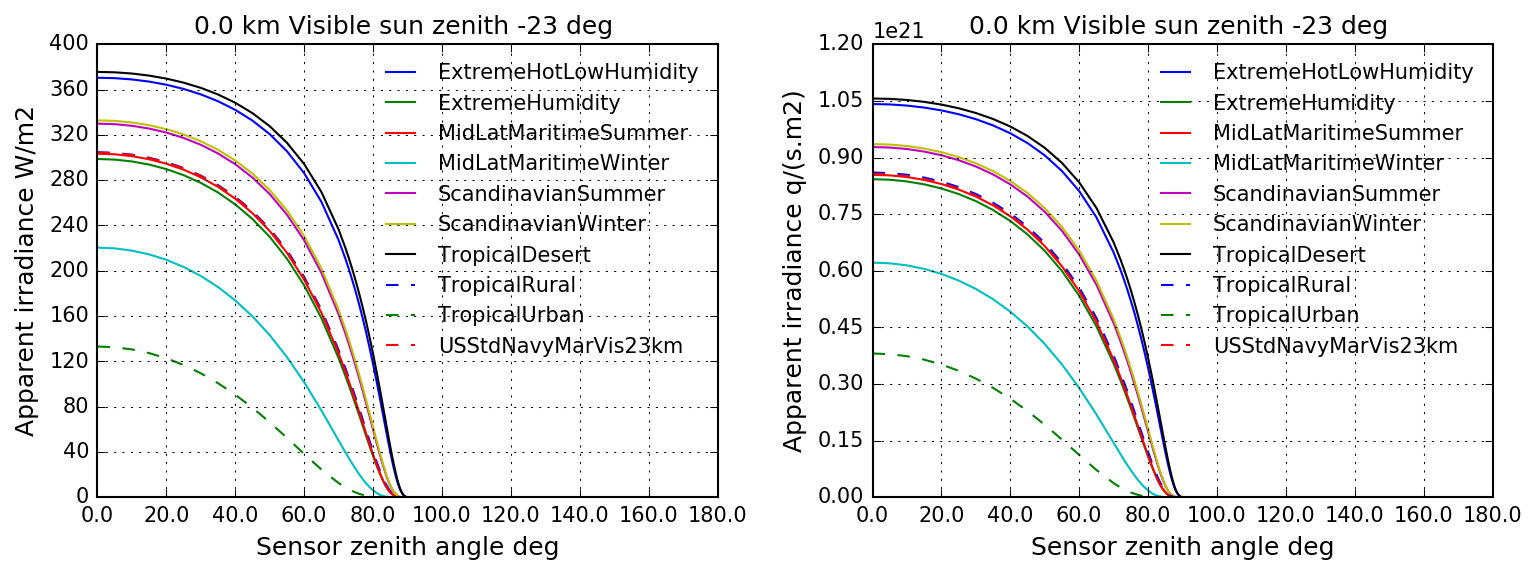
\includegraphics{./pic/Analyse-Standard-Atmospheres_40_0.png}
\end{center}

\begin{center}
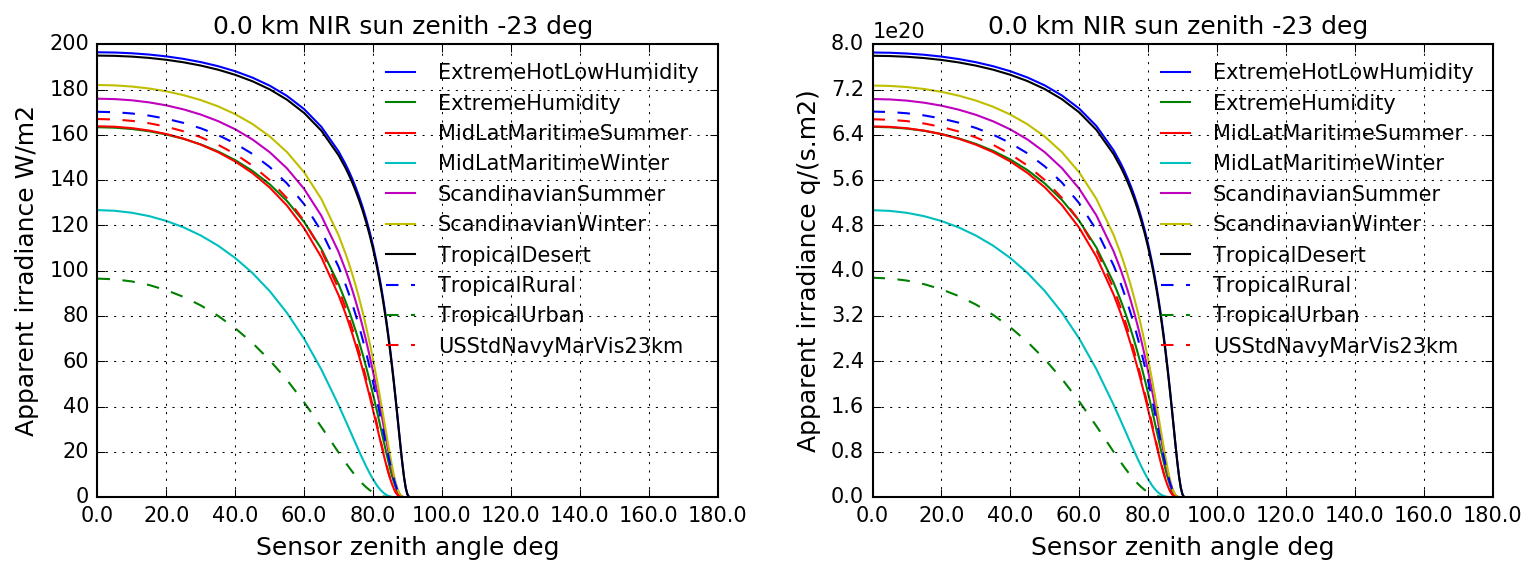
\includegraphics{./pic/Analyse-Standard-Atmospheres_40_1.png}
\end{center}

\begin{center}
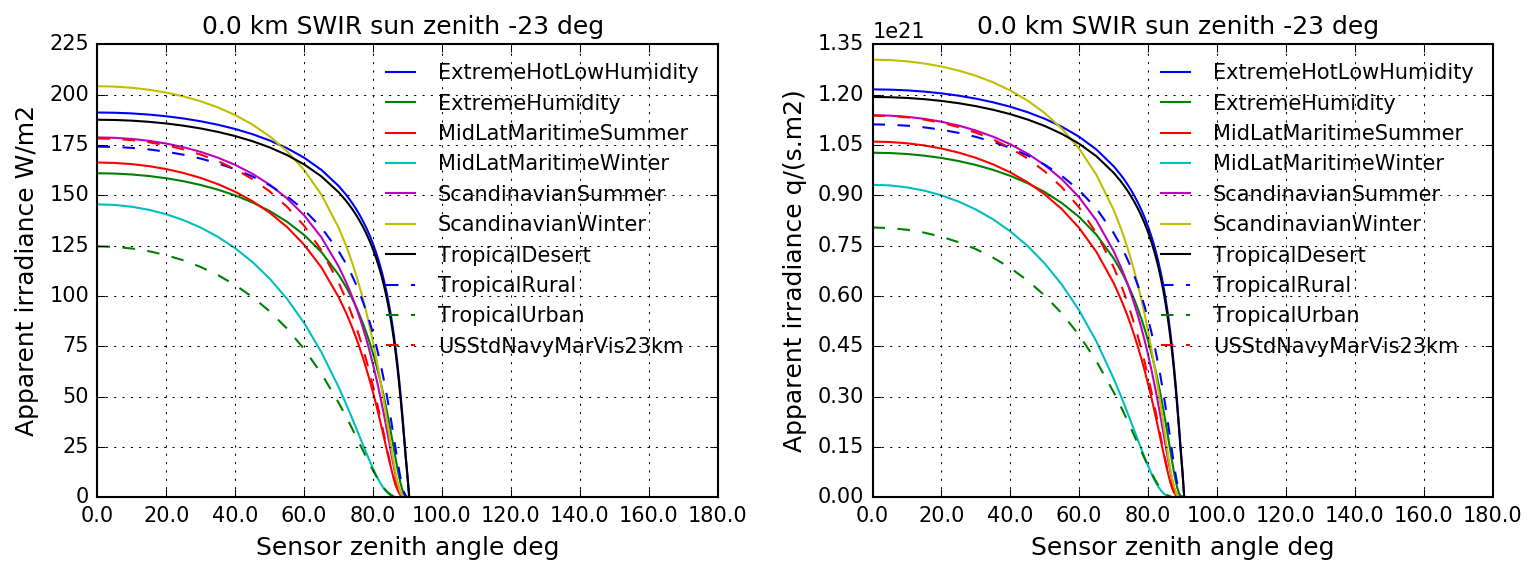
\includegraphics{./pic/Analyse-Standard-Atmospheres_40_2.png}
\end{center}

\begin{center}
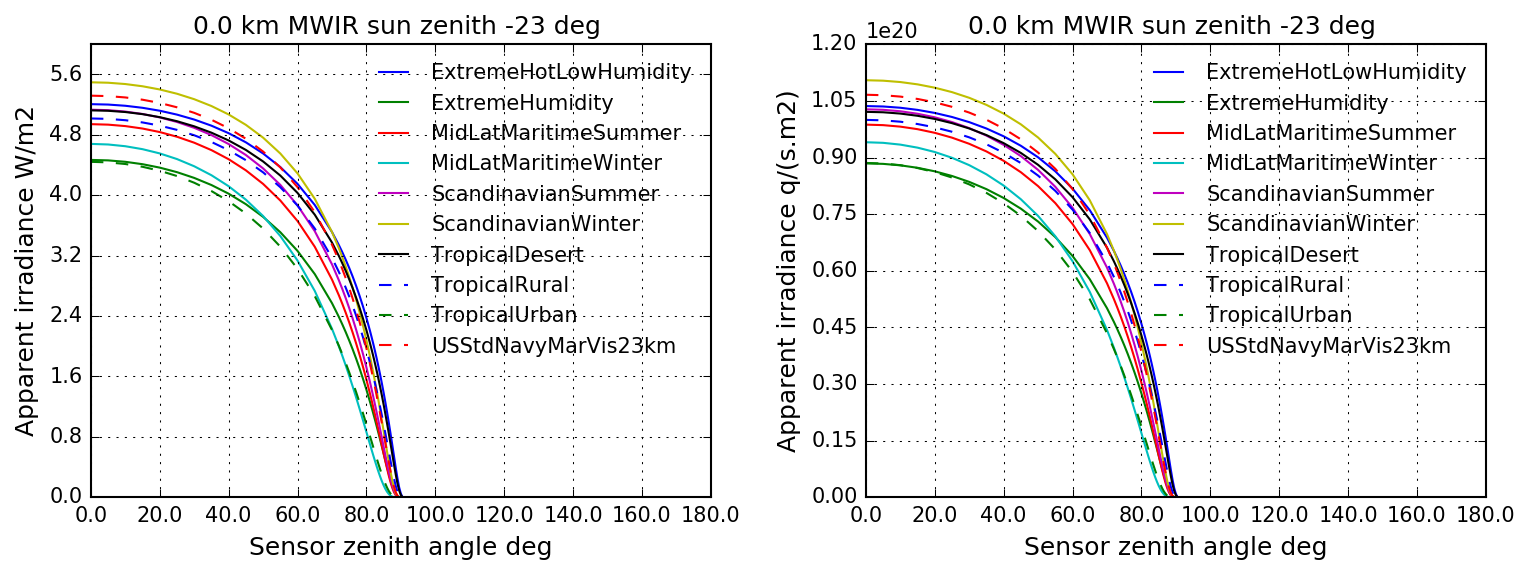
\includegraphics{./pic/Analyse-Standard-Atmospheres_40_3.png}
\end{center}

\begin{center}
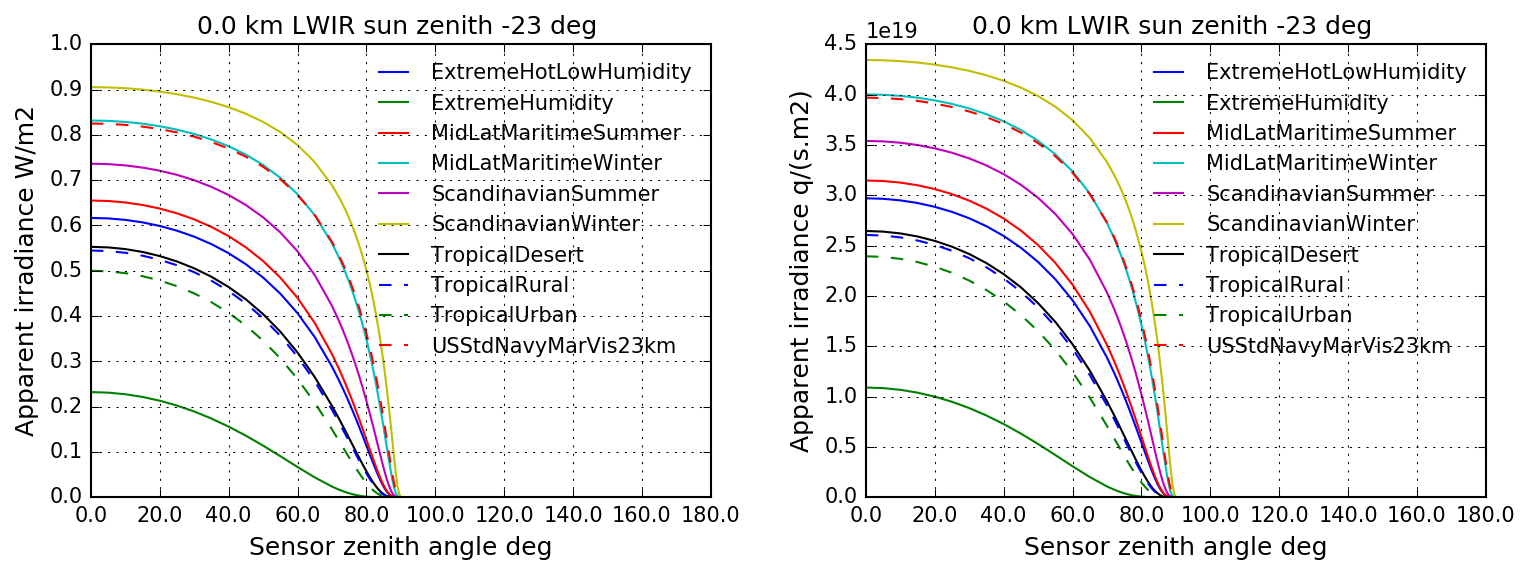
\includegraphics{./pic/Analyse-Standard-Atmospheres_40_4.png}
\end{center}

The next set of graphs show the path radiance for the different spectral bands and for different altitudes. At zero altitude only zenith angles above the horizon are displayed.  At high altitudes the path radiance for all lookup and lookdown angles are displayed.


\begin{enumerate}
\item Vis/NIR/SWIR:  The atmospheres with high aerosol content has high  path radiance closer to the vertical (nearer the sun), whereas the atmospheres with low aerosol content has lower path radiance near the vertical.  The ratio in path radiance near the vertical is more than double (closer to the sun it will be even higher).
\item Vis/NIR/SWIR: At  zenith angles more than 40 degrees from the sun, there is relatively little difference in path radiance between the different atmospheres, except near the horizon where aerosol differences lead to differences in path radiance.
\item Vis/NIR/SWIR: Towards the horizon the path radiance of high aerosol atmospheres is \textit{lower} than low aerosol atmosphere path radiance. Visually, I suspect that with aerosol atmospheres will have a white/grey horizon, whereas a high aerosol atmosphere has a red/brown horizon.  This is probably because high aerosol atmospheres already lost much of the sunlight in the halo around the sun, with less photons available on the horizon.
\item MWIR/LWIR: the path radiance near the sun or at small zenith angles is relatively small compared to the  path radiance nearer the horizon.  The atmospheric temperature plays a major role: hot atmospheres have higher path radiance.  Winter atmospheres have MWIR path radiance generally below 0.5 W/(m\textsuperscript{2}.sr), whereas the really hot atmospheres have MWIR path radiance exceeding 1 W/(m\textsuperscript{2}.sr).
\item The MWIR path radiance is less strongly affected by absolute humidity, and more by temperature.
\item The LWIR path radiance is strongly affected by absolute humidity, but also by temperature (keep in mind that atmospheres at higher temperatures allows higher absolute humidity).
\end{enumerate}



See Listing~\ref{lst:autolistingcell42} for the code to plot the path radiance for the different spectral bands.

\begin{center}
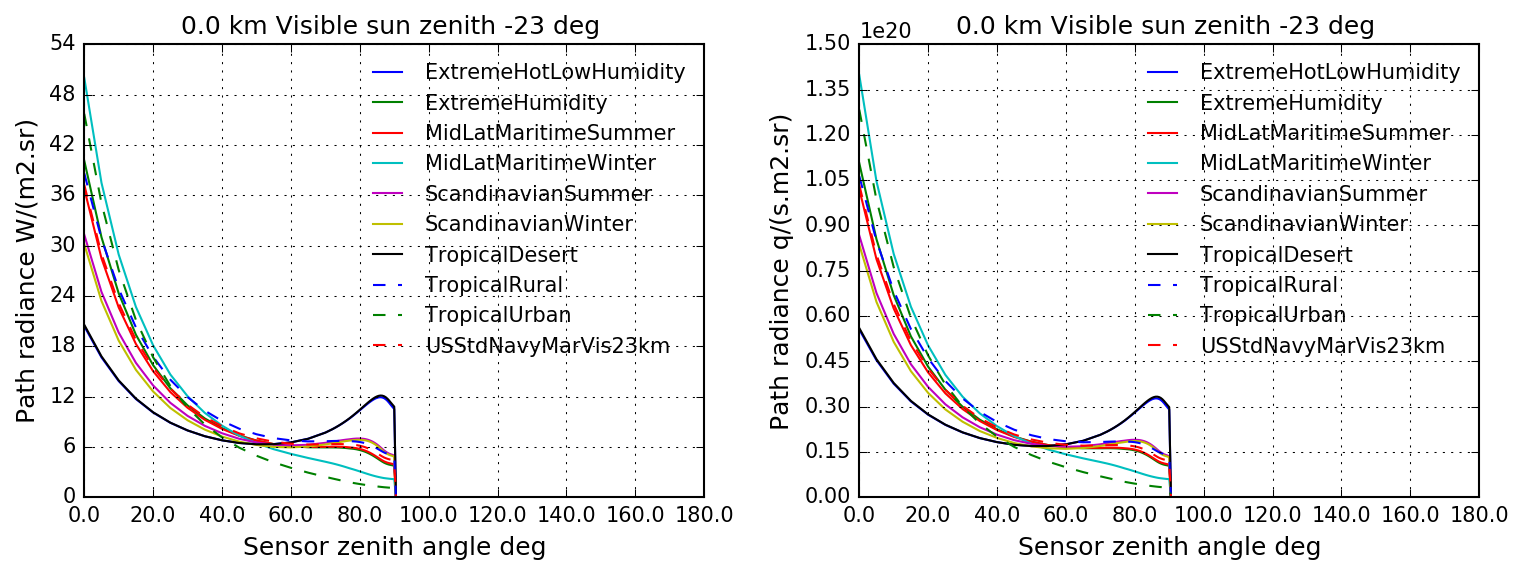
\includegraphics{./pic/Analyse-Standard-Atmospheres_42_0.png}
\end{center}

\begin{center}
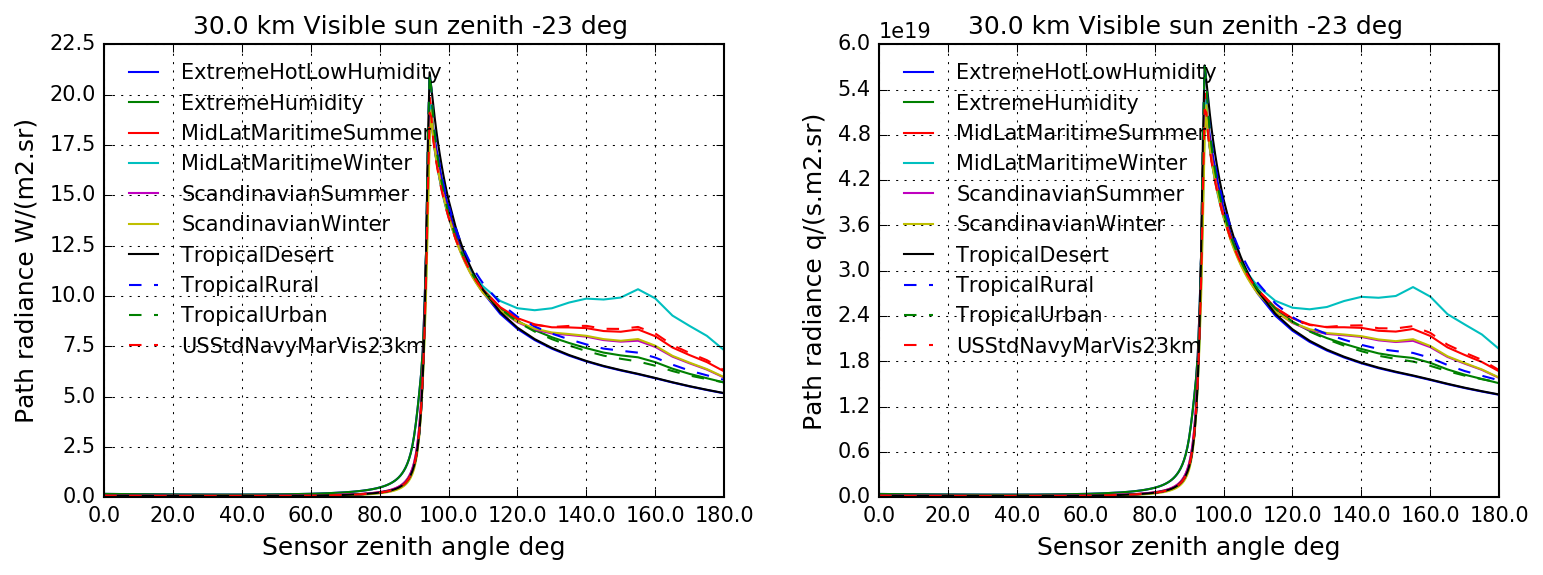
\includegraphics{./pic/Analyse-Standard-Atmospheres_42_1.png}
\end{center}

\begin{center}
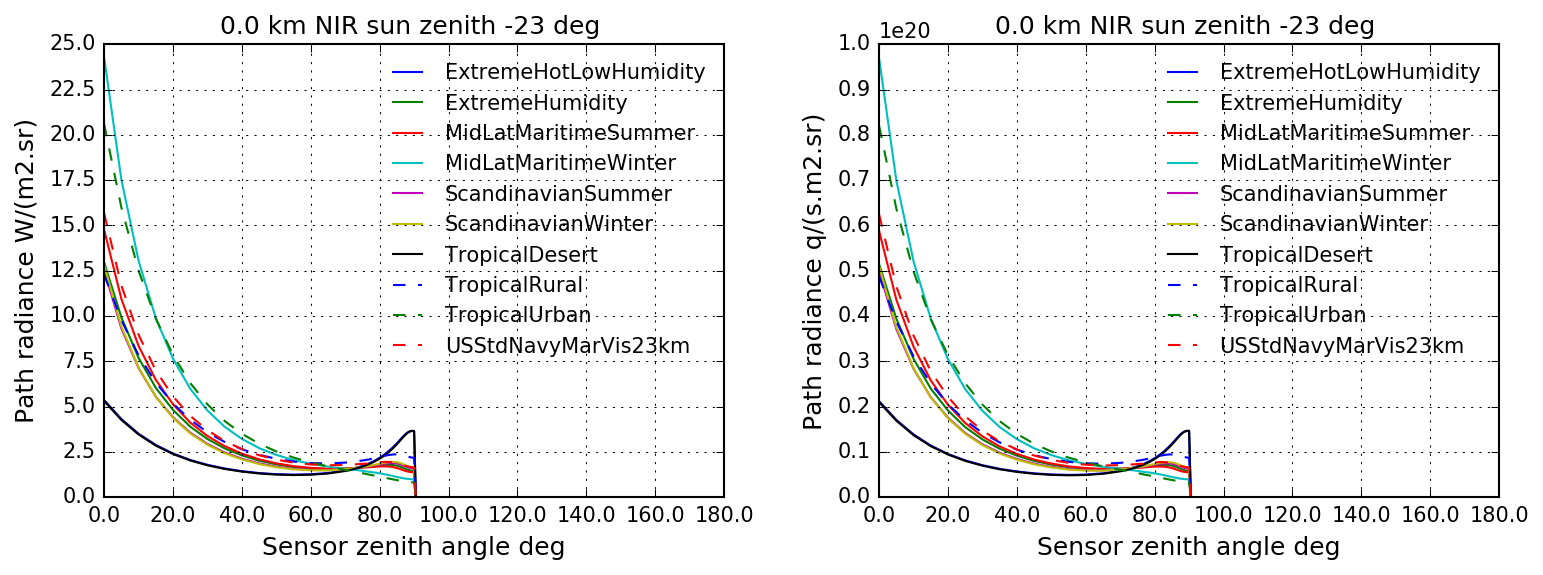
\includegraphics{./pic/Analyse-Standard-Atmospheres_42_2.png}
\end{center}

\begin{center}
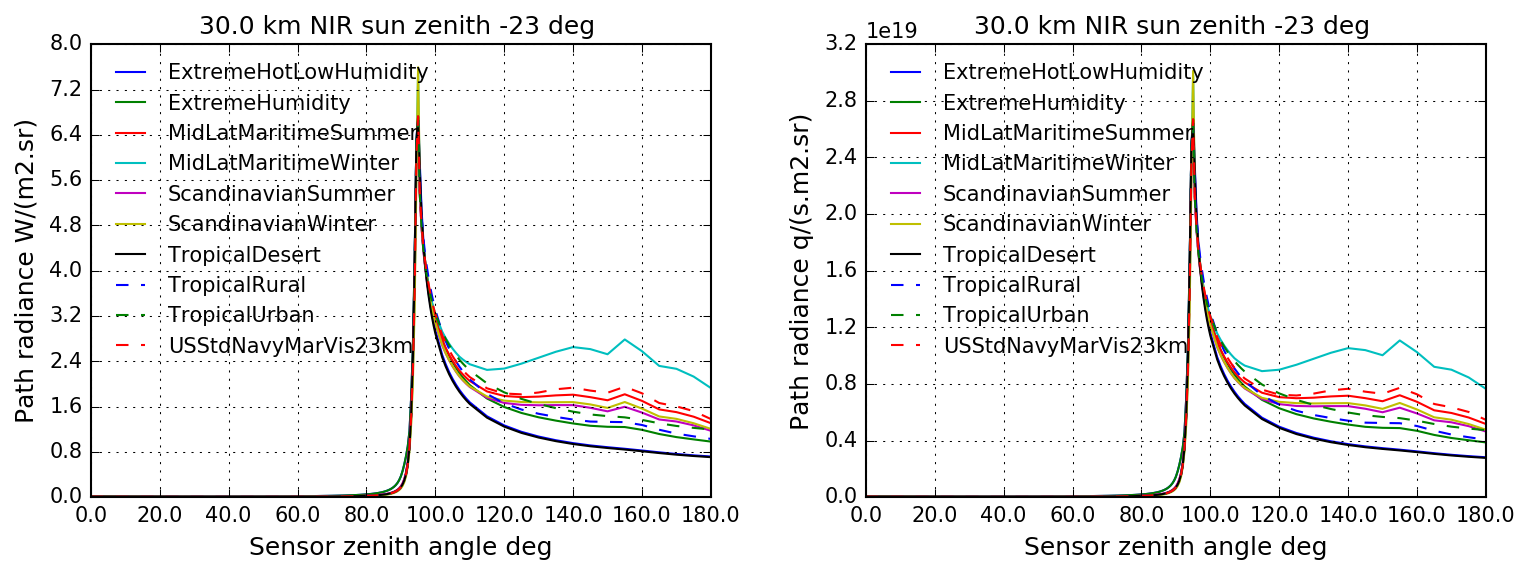
\includegraphics{./pic/Analyse-Standard-Atmospheres_42_3.png}
\end{center}

\begin{center}
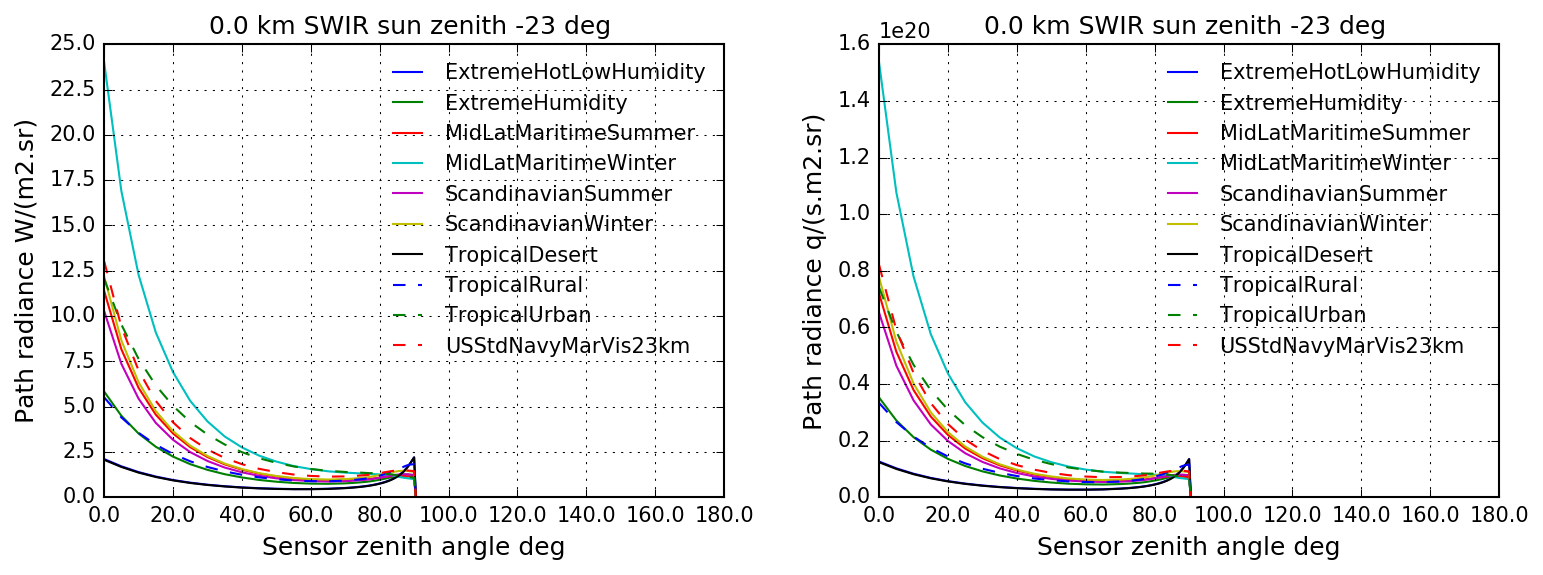
\includegraphics{./pic/Analyse-Standard-Atmospheres_42_4.png}
\end{center}

\begin{center}
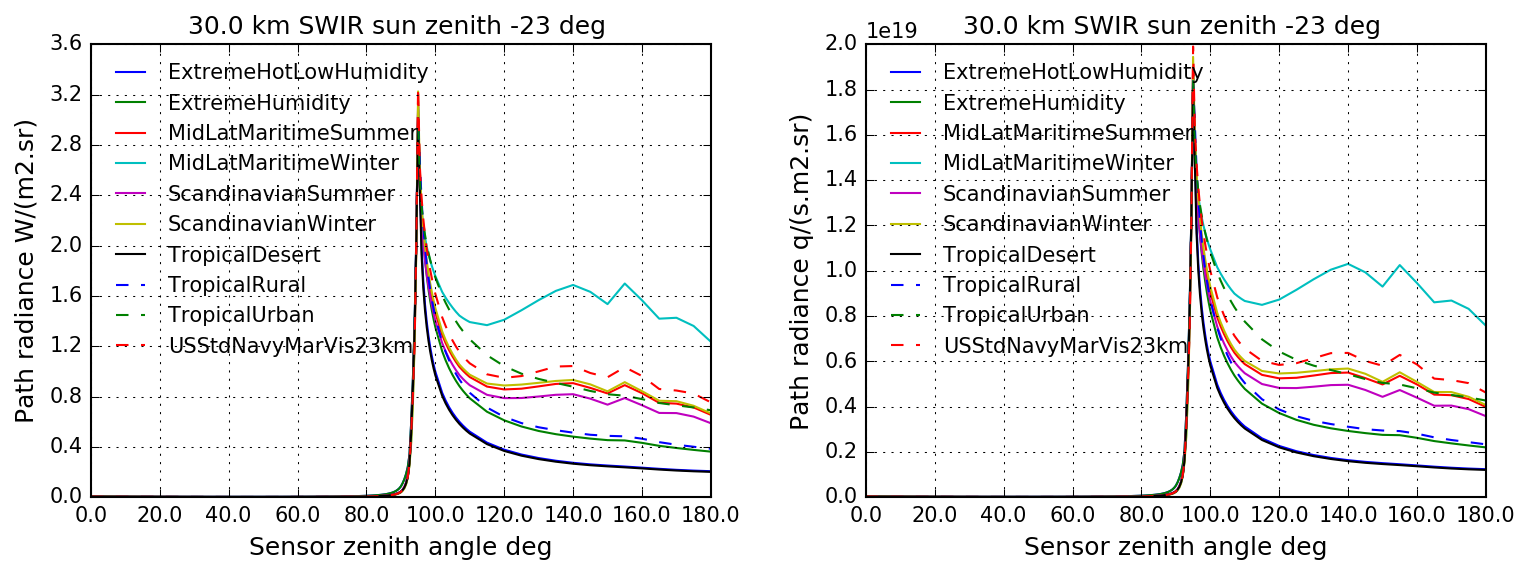
\includegraphics{./pic/Analyse-Standard-Atmospheres_42_5.png}
\end{center}

\begin{center}
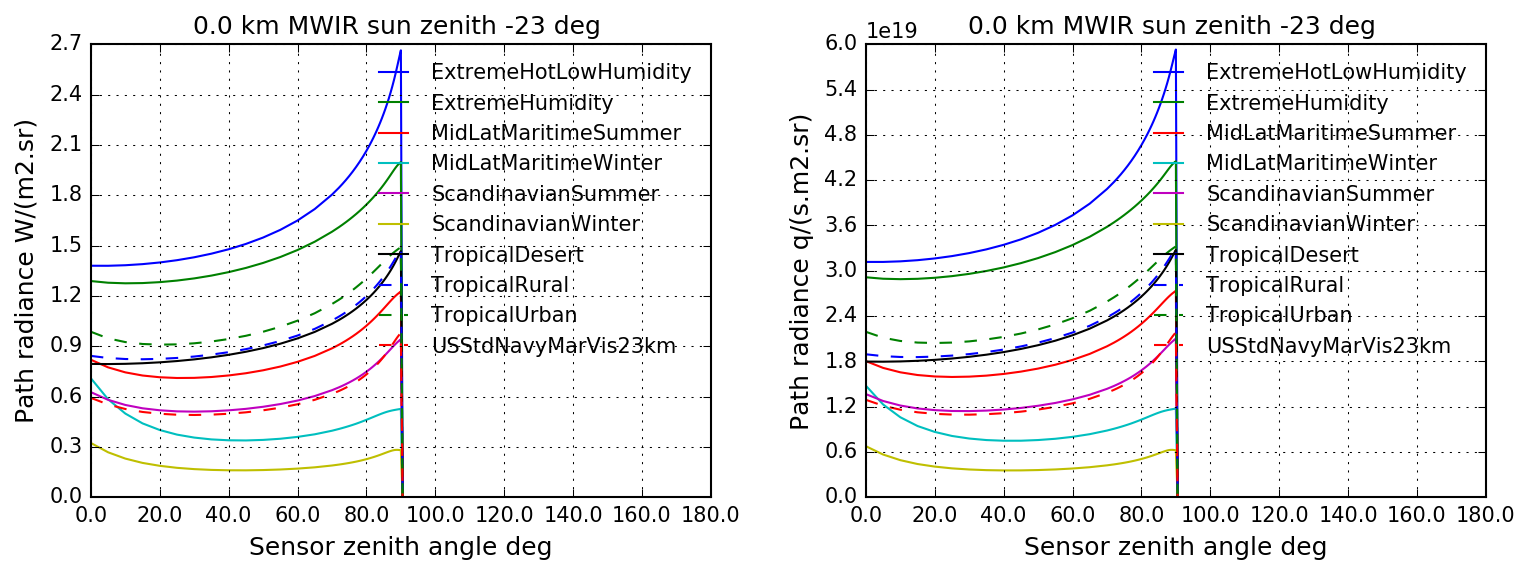
\includegraphics{./pic/Analyse-Standard-Atmospheres_42_6.png}
\end{center}

\begin{center}
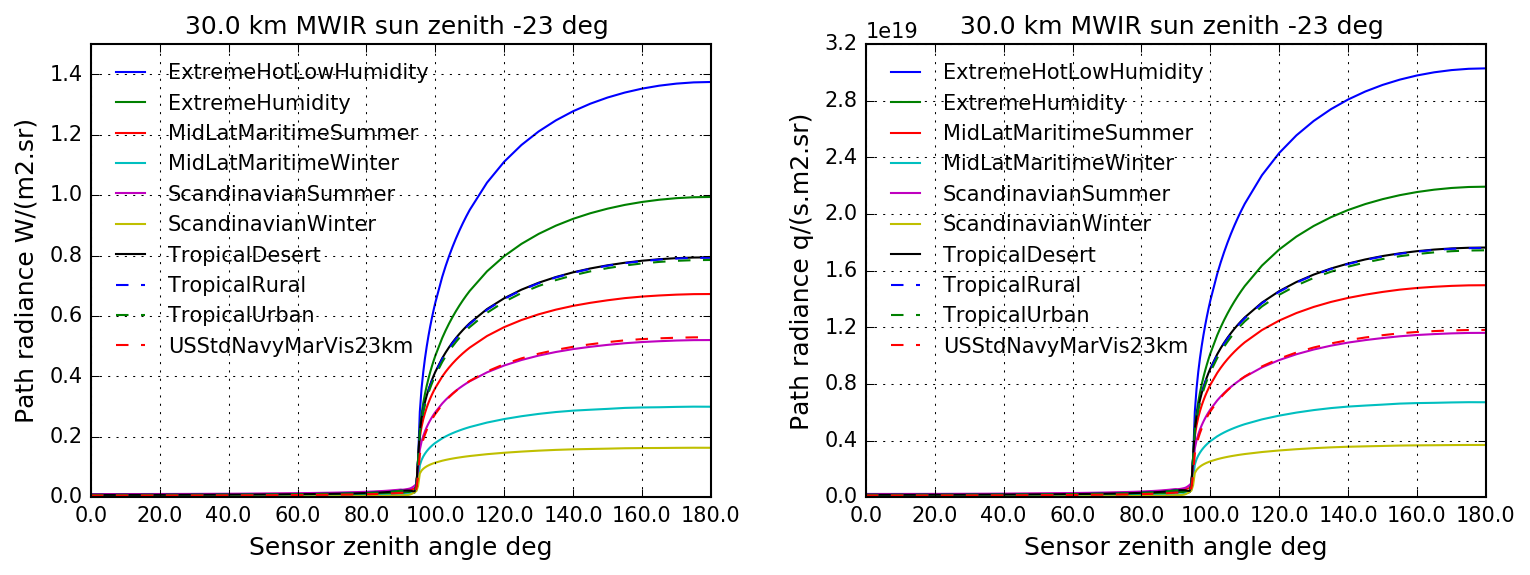
\includegraphics{./pic/Analyse-Standard-Atmospheres_42_7.png}
\end{center}

\begin{center}
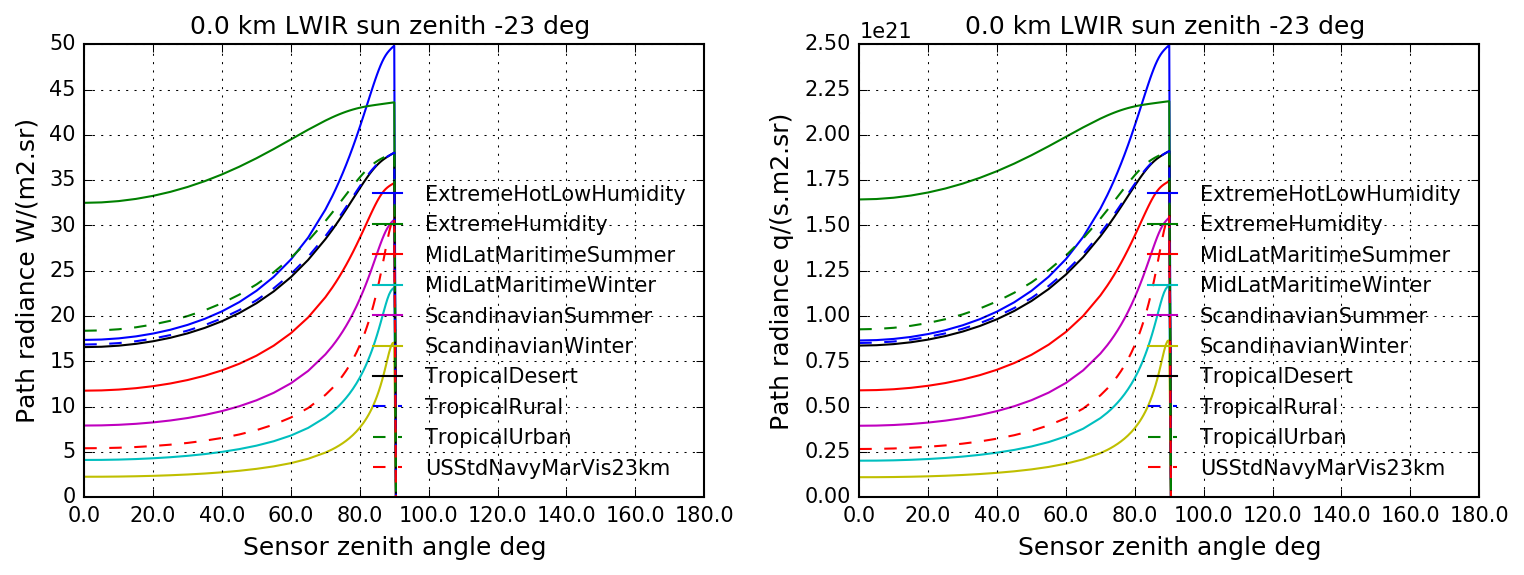
\includegraphics{./pic/Analyse-Standard-Atmospheres_42_8.png}
\end{center}

\begin{center}
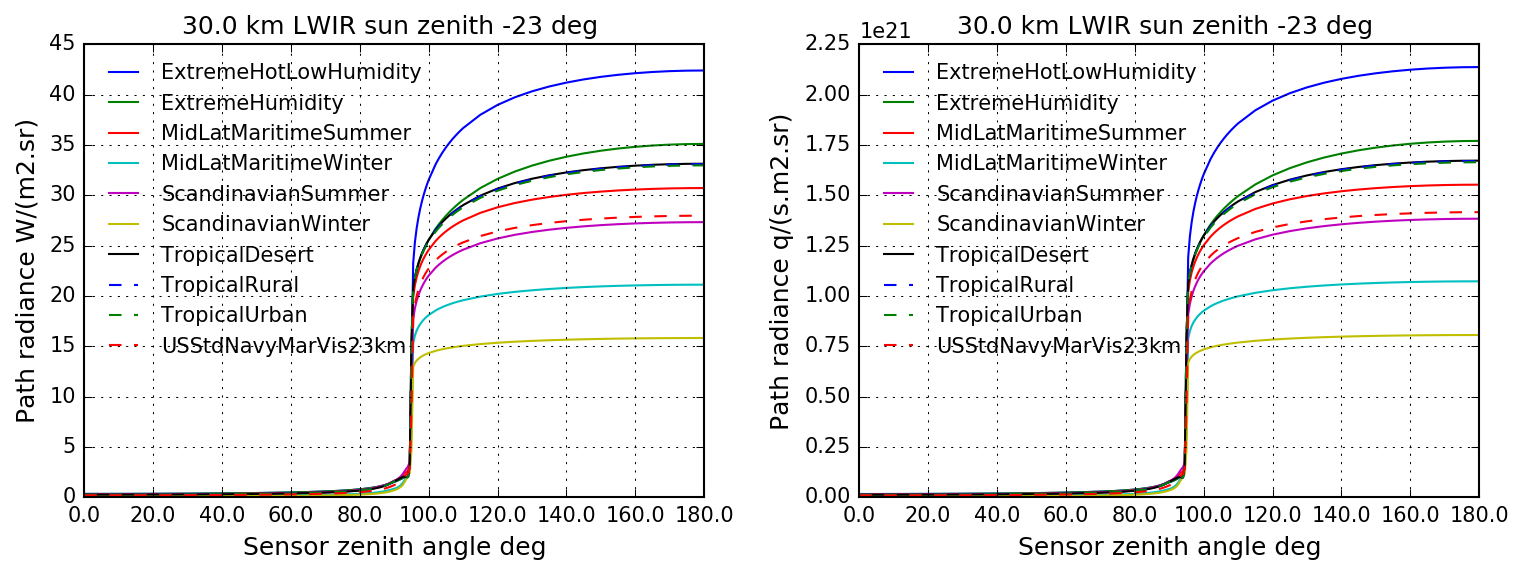
\includegraphics{./pic/Analyse-Standard-Atmospheres_42_9.png}
\end{center}



See Listing~\ref{lst:autolistingcell43} for the code to plot the effective transmittance for the different atmospheres.

\begin{center}
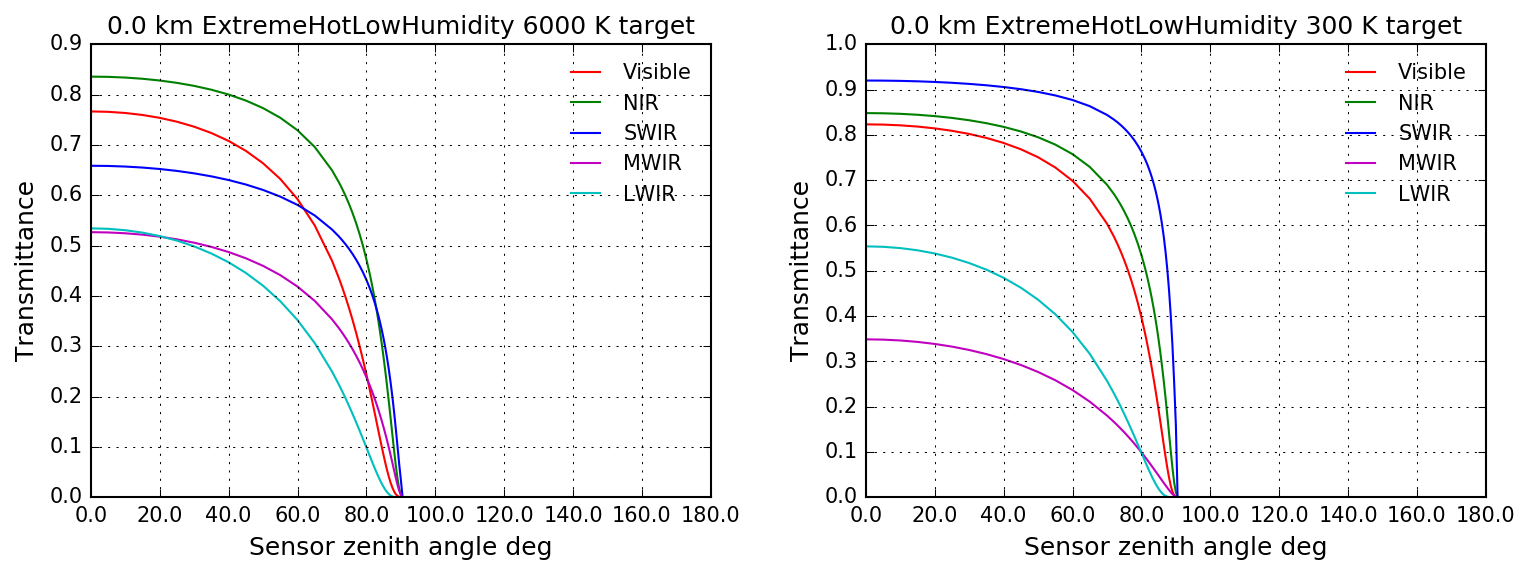
\includegraphics{./pic/Analyse-Standard-Atmospheres_43_0.png}
\end{center}

\begin{center}
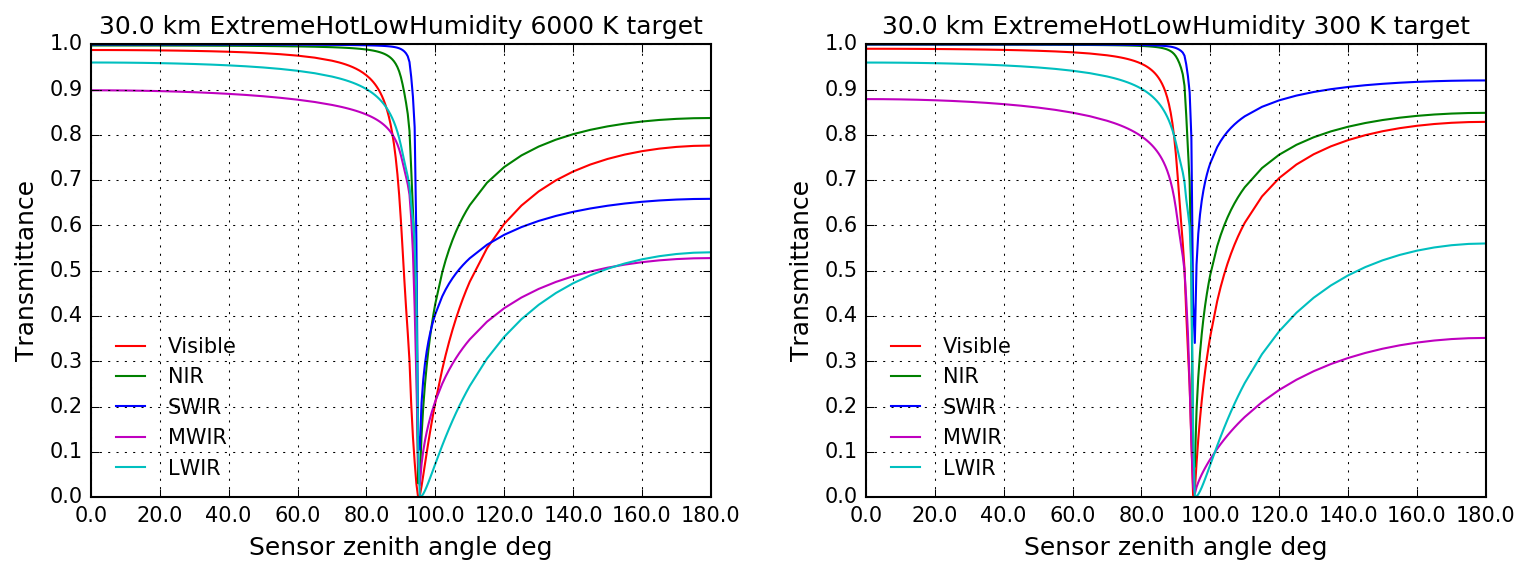
\includegraphics{./pic/Analyse-Standard-Atmospheres_43_1.png}
\end{center}

\begin{center}
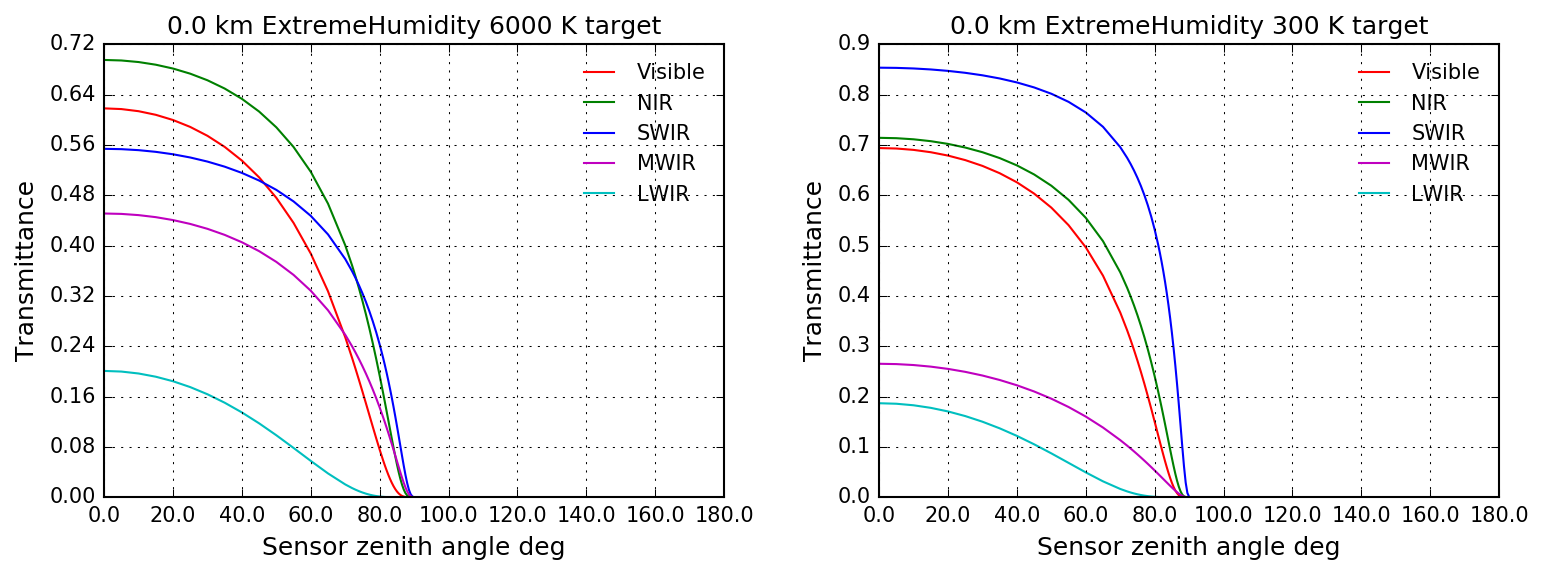
\includegraphics{./pic/Analyse-Standard-Atmospheres_43_2.png}
\end{center}

\begin{center}
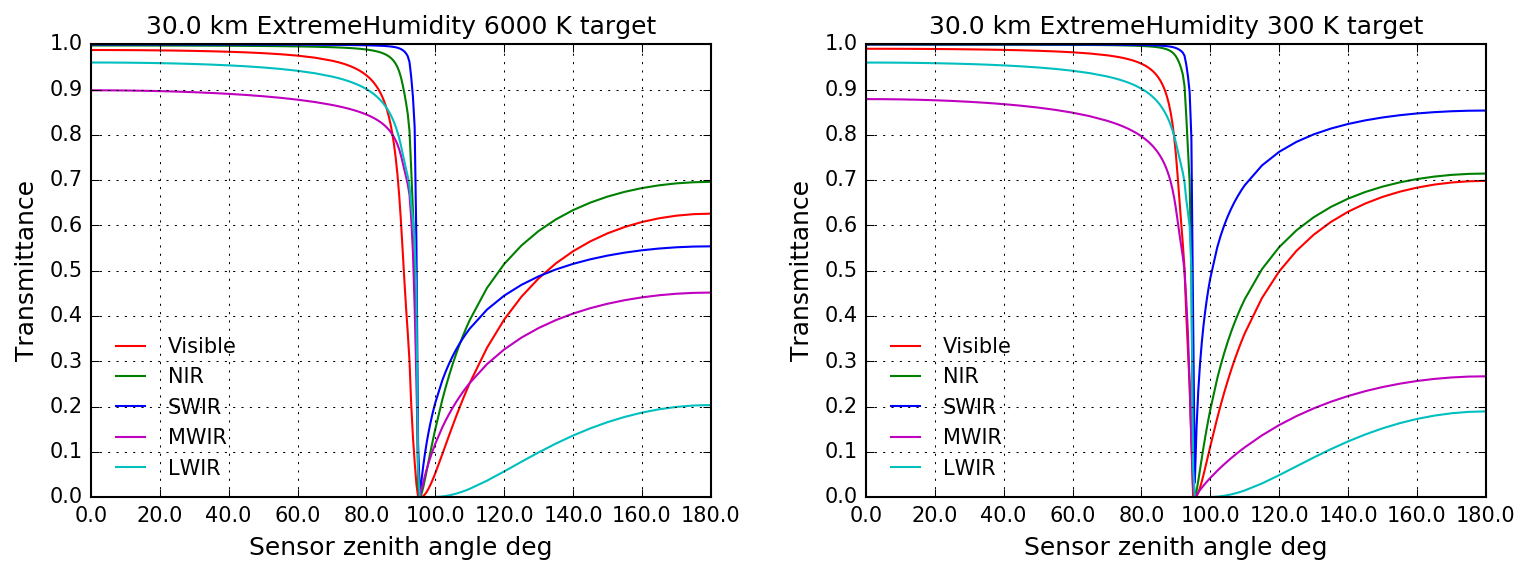
\includegraphics{./pic/Analyse-Standard-Atmospheres_43_3.png}
\end{center}

\begin{center}
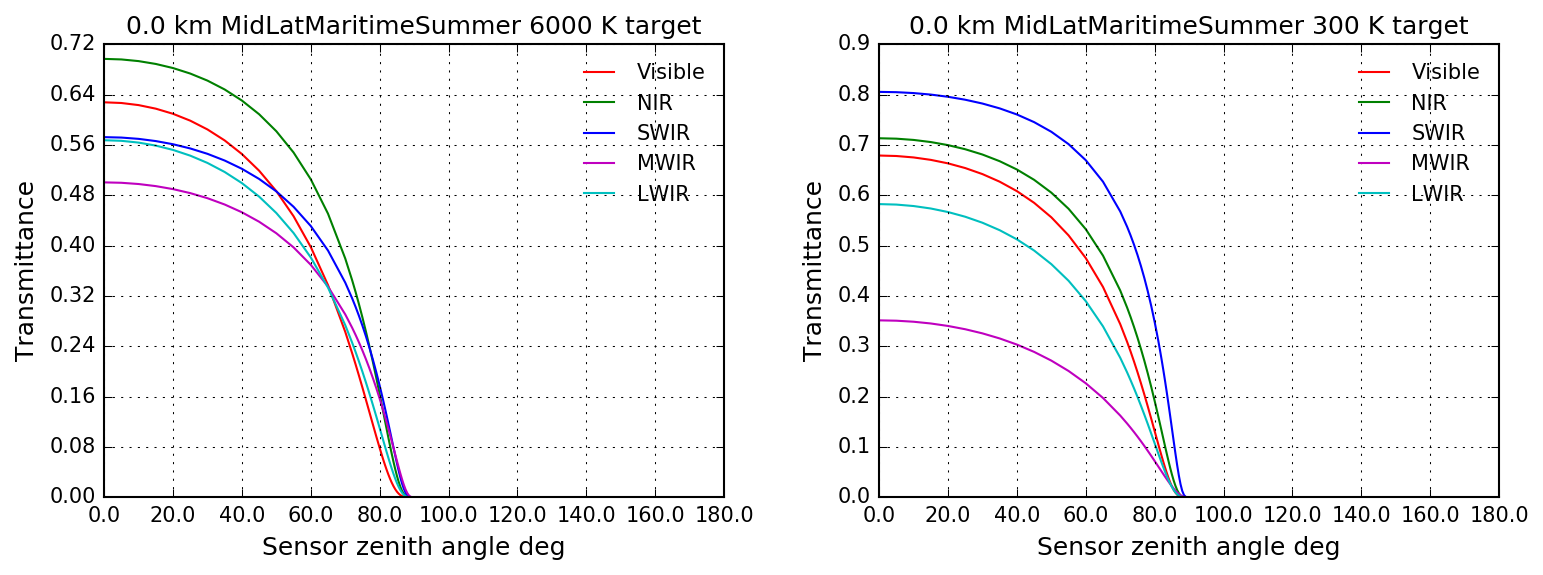
\includegraphics{./pic/Analyse-Standard-Atmospheres_43_4.png}
\end{center}

\begin{center}
\includegraphics{./pic/Analyse-Standard-Atmospheres_43_5.png}
\end{center}

\begin{center}
\includegraphics{./pic/Analyse-Standard-Atmospheres_43_6.png}
\end{center}

\begin{center}
\includegraphics{./pic/Analyse-Standard-Atmospheres_43_7.png}
\end{center}

\begin{center}
\includegraphics{./pic/Analyse-Standard-Atmospheres_43_8.png}
\end{center}

\begin{center}
\includegraphics{./pic/Analyse-Standard-Atmospheres_43_9.png}
\end{center}

\begin{center}
\includegraphics{./pic/Analyse-Standard-Atmospheres_43_10.png}
\end{center}

\begin{center}
\includegraphics{./pic/Analyse-Standard-Atmospheres_43_11.png}
\end{center}

\begin{center}
\includegraphics{./pic/Analyse-Standard-Atmospheres_43_12.png}
\end{center}

\begin{center}
\includegraphics{./pic/Analyse-Standard-Atmospheres_43_13.png}
\end{center}

\begin{center}
\includegraphics{./pic/Analyse-Standard-Atmospheres_43_14.png}
\end{center}

\begin{center}
\includegraphics{./pic/Analyse-Standard-Atmospheres_43_15.png}
\end{center}

\begin{center}
\includegraphics{./pic/Analyse-Standard-Atmospheres_43_16.png}
\end{center}

\begin{center}
\includegraphics{./pic/Analyse-Standard-Atmospheres_43_17.png}
\end{center}

\begin{center}
\includegraphics{./pic/Analyse-Standard-Atmospheres_43_18.png}
\end{center}

\begin{center}
\includegraphics{./pic/Analyse-Standard-Atmospheres_43_19.png}
\end{center}



See Listing~\ref{lst:autolistingcell44} for the code to plot the effective transmittance for the different spectral bands.

\begin{center}
\includegraphics{./pic/Analyse-Standard-Atmospheres_44_0.png}
\end{center}

\begin{center}
\includegraphics{./pic/Analyse-Standard-Atmospheres_44_1.png}
\end{center}

\begin{center}
\includegraphics{./pic/Analyse-Standard-Atmospheres_44_2.png}
\end{center}

\begin{center}
\includegraphics{./pic/Analyse-Standard-Atmospheres_44_3.png}
\end{center}

\begin{center}
\includegraphics{./pic/Analyse-Standard-Atmospheres_44_4.png}
\end{center}

\begin{center}
\includegraphics{./pic/Analyse-Standard-Atmospheres_44_5.png}
\end{center}

\begin{center}
\includegraphics{./pic/Analyse-Standard-Atmospheres_44_6.png}
\end{center}

\begin{center}
\includegraphics{./pic/Analyse-Standard-Atmospheres_44_7.png}
\end{center}

\begin{center}
\includegraphics{./pic/Analyse-Standard-Atmospheres_44_8.png}
\end{center}

\begin{center}
\includegraphics{./pic/Analyse-Standard-Atmospheres_44_9.png}
\end{center}


\chapter{$\alpha$, $\beta$  and $\gamma$ fits to standard atmospheres}
\label{sec:alphabetaandgammafitstostandardatmospheres}

Clients sometimes use simple equations to model atmospheric transmittance with range.  These models are not suitable for wideband spectral ranges.  This section investigates the goodness of fit of two such models.  Both these models apply for a uniform atmospheric path. Slant paths from any height above 2 km would not be accurately modelled.


The $(\alpha,\beta)$ extinction model  is as follows:\begin{equation}\tau = \exp{\left[-\alpha R \left( \frac{10}{R}\right)^\beta \right]}\end{equation}


The $(\gamma)$  or Beer (Bouguer) extinction model  is as follows:\begin{equation}\tau = \exp{\left[-\gamma R \right]}\end{equation}


In the graph below the curves labelled 'Effective Transmittance' are the true transmittance variation against range.  The sets of curves labelled '$\alpha/\beta$ and $\gamma$ are the approximation curve fits.


It is quite evident that the approximation curves are not very good approximations.  For the data shown here the $(\alpha,\beta)$ extinction model gives a reasonable fit over the distances considered (0.1 to 15 km), but beyond 15 km the error grows very quickly.  The $(\gamma)$ model only fits reasonably for a path length shorter than about 2 km.




See Listing~\ref{lst:autolistingcell46} for the code to model the approximations.



See Listing~\ref{lst:autolistingcell47} for the code to collect list of atmospheres.



See Listing~\ref{lst:autolistingcell48} for the code to plot the approximations vs true results..

\begin{center}
\includegraphics{./pic/Analyse-Standard-Atmospheres_48_0.png}
\end{center}



See Listing~\ref{lst:autolistingcell49} for the code to prepare tables.

\begin{center}

\begin{footnotesize}

\begin{tabular}{|c|c|c|c|c|}
\hline
&Atmosphere&$\alpha$&$\beta$&$\gamma$\\\hline
0&ExtremeHotLowHumidity: 44 C, 30\% RH (18.1), 77 km Vis Desert&0.270773&0.498202&0.594155\\\hline
1&ExtremeHumidity: 35 C, 95\% RH (37.9), 23 km Vis Rural&0.347705&0.481553&0.919896\\\hline
2&MidLatMaritimeSummer: 21 C, 76\% RH (14), 23 km Vis Maritime&0.322575&0.386728&0.584343\\\hline
3&MidLatMaritimeWinter: -1 C, 77\% RH (3), 10 km Vis Maritime&0.346758&0.270231&0.498239\\\hline
4&ScandinavianSummer: 14 C, 75\% RH (9), 31 km Vis Maritime&0.282606&0.383870&0.465228\\\hline
5&ScandinavianWinter: -15.9 C, 80\% RH (1), 31 km Vis Maritime&0.202865&0.348069&0.260869\\\hline
6&TropicalDesert: 26.6 C, 75\% RH (18), 75 km Vis Desert&0.271947&0.480195&0.564427\\\hline
7&TropicalRural: 26.6 C, 75\% RH (18), 23 km Vis Rural&0.287227&0.461126&0.590823\\\hline
8&TropicalUrban: 26.6 C, 75\% RH (18), 5 km Vis Urban&0.388425&0.364487&0.743685\\\hline
9&USStdNavyMarVis23km: 15 C, 46\% RH (5.9), 23 km Vis Nav.Mar, SS4&0.254076&0.383958&0.390133\\\hline

\end{tabular}
\end{footnotesize}
\end{center}


\chapter{Python and module versions, and dates}
\label{sec:Pythonandmoduleversionsanddates}

See Listing~\ref{lst:autolistingcell51} for the code.

\begin{center}

\begin{normalsize}

\begin{tabular}{|c|c|}
\hline
Software&Version\\\hline
Python&2.7.11 64bit [MSC v.1500 64 bit (AMD64)]\\\hline
IPython&4.1.2\\\hline
OS&Windows 7 6.1.7601 SP1\\\hline
numpy&1.10.4\\\hline
scipy&0.17.0\\\hline
matplotlib&1.5.1\\\hline
pyradi&0.2.3\\\hline
pandas&0.18.0\\\hline
\multicolumn{2}{|c|}{Mon Sep 26 09:20:16 2016 South Africa Standard Time}\\\hline

\end{tabular}
\end{normalsize}
\end{center}


\begin{lstlisting}[style=outcellstyle]
Software versions
Python 2.7.11 64bit [MSC v.1500 64 bit (AMD64)]
IPython 4.1.2
OS Windows 7 6.1.7601 SP1
numpy 1.10.4
scipy 0.17.0
matplotlib 1.5.1
pyradi 0.2.3
pandas 0.18.0
Mon Sep 26 09:20:16 2016 South Africa Standard Time
\end{lstlisting}



\chapter{Listings}


\begin{lstlisting}[style=incellstyle,caption={Code Listing in cell 10 \label{lst:autolistingcell10}}]
#to prepare the environment
import numpy as np
import scipy as sp
import pandas as pd
import pyradi.ryplot as ryplot
import os.path
from scipy.optimize import curve_fit

%matplotlib inline

# %reload_ext autoreload
# %autoreload 2

import pyradi.ryplot as ryplot
import pyradi.ryplanck as ryplanck
import pyradi.ryfiles as ryfiles
import pyradi.rymodtran as rymodtran

# import xlsxwriter

from IPython.display import HTML
from IPython.display import Image
from IPython.display import display
from IPython.display import FileLink, FileLinks

#make pngs at 150 dpi
import matplotlib as mpl
mpl.rc("savefig", dpi=150)
mpl.rc('figure', figsize=(10,8))
# %config InlineBackend.figure_format = 'svg'

pd.set_option('display.max_columns', 80)
pd.set_option('display.width', 200)
pd.set_option('display.max_colwidth', 150)


\end{lstlisting}


\begin{lstlisting}[style=incellstyle,caption={Code Listing in cell 12 \label{lst:autolistingcell12}}]
#to define the atmospheres
"""This file provides Python-style definitions of the standard atmospheres.
This file can be included in other python scripts
"""

#each base tape5 file is in its own directory
dirs = ['ExtremeHotLowHumidity', 'ExtremeHumidity',
        'MidLatMaritimeSummer','MidLatMaritimeWinter',
        'ScandinavianSummer','ScandinavianWinter',
        'TropicalDesert','TropicalRural',
        'TropicalUrban','USStdNavyMarVis23km']
        
#altitudes  (in m)
alts = [305, 1524, 3048, 4572, 6096, 7620, 9144, 10668, 12192, 13716, 14326, 15240]
              
atmospheres = {
    u'ExtremeHotLowHumidity':['44 C, 30% RH (18.1), 77 km Vis Desert'],
    u'ExtremeHumidity'      :['35 C, 95% RH (37.9), 23 km Vis Rural'],
    u'MidLatMaritimeSummer' :['21 C, 76% RH (14), 23 km Vis Maritime'],
    u'MidLatMaritimeWinter' :['-1 C, 77% RH (3), 10 km Vis Maritime'],
    u'ScandinavianSummer'   :['14 C, 75% RH (9), 31 km Vis Maritime'],
    u'ScandinavianWinter'   :['-15.9 C, 80% RH (1), 31 km Vis Maritime'],
    u'TropicalDesert'       :['26.6 C, 75% RH (18), 75 km Vis Desert'], 
    u'TropicalRural'        :['26.6 C, 75% RH (18), 23 km Vis Rural'],
    u'TropicalUrban'        :['26.6 C, 75% RH (18), 5 km Vis Urban'],
    u'USStdNavyMarVis23km'  :['15 C, 46% RH (5.9), 23 km Vis Nav.Mar, SS4'],
    }

\end{lstlisting}


\begin{lstlisting}[style=incellstyle,caption={Code Listing in cell 15 \label{lst:autolistingcell15}}]
#to plot the vertical profiles
def plotProfiles(alts, dirs, atmospheres,maxalt):
    #first plot the different altitudes for each atmosphere
    pa = ryplot.Plotter(4, 1, 1, figsize=(6,6));
    pp = ryplot.Plotter(1, 1, 1, figsize=(6,6));
    pt = ryplot.Plotter(2, 1, 1, figsize=(6,6));
    ph = ryplot.Plotter(3, 1, 1, figsize=(6,6));
    
    for i,directory in enumerate(dirs):
        for alt in alts:
            if alt == 305:
                datadir = os.path.join('.',directory,'{}'.format(alt))
                filename = os.path.join(datadir,'tape6')
                with open(filename,'rt') as fin:
                    lines = fin.readlines()
                    cntProfiles = 0
                    linecnt = 0
                    doLines = True
                    while(doLines and linecnt < len(lines)):
                        if 'ATMOSPHERIC PROFILES' in lines[linecnt]:
                            linecnt += 2 # discard empty line and read next
                            acclines = []
                            if 'RH (%)' in lines[linecnt]:
                                linecnt += 2 # discard header lines
                                for i in range(36):
                                    acclines.append((lines[linecnt]).split())
                                    linecnt += 1
                                arr = np.asarray(acclines, dtype=np.float)
                                arr[0,1] = .1
                                #write profile to disk
                                profile = np.hstack((arr[:,1].reshape(-1,1),arr[:,2].reshape(-1,1),arr[:,3].reshape(-1,1),arr[:,10].reshape(-1,1)))
                                profilepath = os.path.join('.',directory,'{}-profile.txt'.format(directory))
                                np.savetxt(profilepath, profile)
                                #process
                                arrdf = pd.DataFrame(arr)
                                arrdf = arrdf[arrdf[1] <= maxalt]
                                arr = arrdf.values
                                aero = np.sum(arr[:,4:8], axis=1)
                                pa.logLog(1,aero,arr[:,1],label=[directory])
                                pp.semilogY(1,arr[:,2],arr[:,1],label=[directory])
                                pt.semilogY(1,arr[:,3],arr[:,1],label=[directory])
                                ph.semilogY(1,arr[:,10],arr[:,1],label=[directory])
                                doLines = False
                        linecnt += 1
        
    cpa = pa.getSubPlot(1)
    cpp = pp.getSubPlot(1)
    cpt = pt.getSubPlot(1)
    cph = ph.getSubPlot(1)
    
    for falt in [1000, 5000, 30000]:
        malt = 0.3048 * falt / 1000.
        pa.logLog(1,np.asarray([1e-4,1e0]),np.asarray([malt,malt]),plotCol='k')
        cpa.text(0.2,0.9*malt, '{:.0f} kft'.format(falt/1000.), horizontalalignment='left', fontsize=8)    
        pp.semilogY(1,np.asarray([240,1040]),np.asarray([malt,malt]),plotCol='k')
        cpp.text(960,0.9*malt, '{:.0f} kft'.format(falt/1000.), horizontalalignment='left', fontsize=8)    
        pt.semilogY(1,np.asarray([210,330]),np.asarray([malt,malt]),plotCol='k')
        cpt.text(318,0.9*malt, '{:.0f} kft'.format(falt/1000.), horizontalalignment='left', fontsize=8)    
        ph.semilogY(1,np.asarray([10,100]),np.asarray([malt,malt]),plotCol='k')
        cph.text(92,0.9*malt, '{:.0f} kft'.format(falt/1000.), horizontalalignment='left', fontsize=8)    

    for ext in np.logspace(-2,0, 20):#[1e-2, 1e-1, 1]:
        cpa.text(ext,0.105, '{:.0f} km vis'.format(3.91/ext), verticalalignment='bottom', horizontalalignment='center', fontsize=8, rotation=90)        
        
    cpa.set_xlabel('Extinction [km$^{-1}$]')
    cpa.set_ylabel('Altitude [km]')
    cpa.set_title('Vertical 550 nm Extinction Profiles')
    cpp.set_xlabel('Pressure [mBar]')
    cpp.set_ylabel('Altitude [km]')
    cpp.set_title('Vertical Pressure Profiles')
    cpt.set_xlabel('Temperature [K]')
    cpt.set_ylabel('Altitude [km]')
    cpt.set_title('Vertical Temperature Profiles')
    cph.set_xlabel('Relative humidity [%]')
    cph.set_ylabel('Altitude [km]')
    cph.set_title('Vertical Humidity Profiles')
#     pa.saveFig('profiles-aerosol.png')
#     pp.saveFig('profiles-pressure.png')
#     pt.saveFig('profiles-temperature.png')
#     ph.saveFig('profiles-humidity.png')
    
plotProfiles(alts, dirs, atmospheres, 10.)    
\end{lstlisting}


\begin{lstlisting}[style=incellstyle,caption={Code Listing in cell 17 \label{lst:autolistingcell17}}]
#to plot the spectral transmittance
def plotTau(alts, dirs, atmospheres):
  #first plot the different altitudes for each atmosphere
  for i,directory in enumerate(dirs):
    p = ryplot.Plotter(i, 1, 1, figsize=(12,6))
    for alt in alts:
      datadir = os.path.join('.',directory,'{}'.format(alt))
      filename = '{}-{}m.1km'.format(directory, alt)
      data = np.loadtxt(os.path.join(datadir,filename), skiprows=1)
      p.plot(1, data[:,0], data[:,1],
        '{} {} 1 km transmittance, 135 deg zenith'.format(directory, atmospheres[directory][0]),
        'Wavelength $\mu$m','Transmittance', label=['{} m'.format(alt)],legendAlpha=0.5)
#     p.saveFig(os.path.join('.',directory,'{}.png'.format(directory)))
    
  #now plot the different atmospheres for each altitude
  for j, alt in enumerate(alts):
    p = ryplot.Plotter(j+len(dirs), 1, 1, figsize=(12,6))
    for i,directory in enumerate(dirs):
      datadir = os.path.join('.',directory,'{}'.format(alt))
      filename = '{}-{}m.1km'.format(directory, alt)
      data = np.loadtxt(os.path.join(datadir,filename), skiprows=1)
      p.plot(1, data[:,0], data[:,1],
        '{} m altitude, 135 deg zenith 1 km transmittance'.format(alt),
        'Wavelength $\mu$m','Transmittance', label=['{} {}'.format(directory, atmospheres[directory][0])],
        legendAlpha=0.5)
#     p.saveFig(os.path.join('.','AllScen-{}m.png'.format(alt)))

plotTau(alts, dirs, atmospheres)
\end{lstlisting}


\begin{lstlisting}[style=incellstyle,caption={Code Listing in cell 20 \label{lst:autolistingcell20}}]
#to return Placnk radiator radiance
def lpathfunc(nu,tbb):
    return  ryplanck.planck(nu,tbb, 'en') / np.pi 
\end{lstlisting}


\begin{lstlisting}[style=incellstyle,caption={Code Listing in cell 21 \label{lst:autolistingcell21}}]
#to calculate and plot atmospheric temperature
files = ryfiles.listFiles(root=r'.', 
                patterns=r'.*tape7', recurse=1, return_folders=0, useRegex=True)

#remove the files with elev in the name
fileslist = []
for filen in files:
    if 'elev' not in filen:
        fileslist.append(filen)


dfAtmoTempCols = ['Atmosphere','Altitude','TmpLoTau','TmpHiTau','3.5-4.8','8.3-12','TmpAve','TmpAll']
dfAtmoTemp = pd.DataFrame(columns=dfAtmoTempCols)

# for i,filename in enumerate([r'C:\WorkA\TAPM\Atmospheres\Standard\ExtremeHotLowHumidity\305\tape7',
#                             r'C:\WorkA\TAPM\Atmospheres\Standard\ExtremeHotLowHumidity\15240\tape7']):
for i,filename in enumerate(fileslist):
    filesplit = filename.split('\\')
    colselect = ['FREQ', 'TOT_TRANS','PTH_THRML']
    tape7 = rymodtran.loadtape7(filename, colselect )
    tape7[:,2] *= 1e4

    genericbands = {
        '10-12,5':[12.5, 10.],  # generic
        '8.33-9.34':[9.34, 8.33],  # generic
        '4.5-5.0':[5.0, 4.5],  # generic
        '3.2-4.5':[4.17, 3.2],  # generic
        }
    camerabands = {    
        '8.33-12.0':[12.0, 8.33], # this is the 8-12 band including 
        '3.5-4.8':[4.8, 3.5], # this is the 3-5 band including CO2
        }
    
    #prepare selection for generic bands
    selectHiTau = np.zeros(tape7[:,0].shape)
    for key in genericbands:
        selectHiTau = np.logical_or(selectHiTau, 
            np.all([ tape7[:,0] >= 1e4/genericbands[key][0], tape7[:,0] <= 1e4/genericbands[key][1]], axis=0))

    selectLoTau = np.logical_not(selectHiTau)
    select3to5 = np.all([ tape7[:,0] >= 1e4/camerabands['3.5-4.8'][0], tape7[:,0] <= 1e4/camerabands['3.5-4.8'][1]], axis=0)
    select8to12 = np.all([ tape7[:,0] >= 1e4/camerabands['8.33-12.0'][0], tape7[:,0] <= 1e4/camerabands['8.33-12.0'][1]], axis=0)
   
    popt, pcov = curve_fit(lpathfunc,tape7[selectHiTau,0], tape7[selectHiTau,2]/(1-tape7[selectHiTau,1]), p0=(250.) )
    tmpHiTau = popt[0]
    popt, pcov = curve_fit(lpathfunc,tape7[selectLoTau,0], tape7[selectLoTau,2]/(1-tape7[selectLoTau,1]), p0=(250.) )
    tmpLoTau = popt[0]
    tmpAve = (tmpHiTau + tmpLoTau) / 2.
    popt, pcov = curve_fit(lpathfunc,tape7[:,0], tape7[:,2]/(1-tape7[:,1]), p0=(250.) )
    tmpAll = popt[0]
    popt, pcov = curve_fit(lpathfunc,tape7[select3to5,0], tape7[select3to5,2]/(1-tape7[select3to5,1]), p0=(250.) )
    tmp3to5 = popt[0]
    popt, pcov = curve_fit(lpathfunc,tape7[select8to12,0], tape7[select8to12,2]/(1-tape7[select8to12,1]), p0=(250.) )
    tmp8to12 = popt[0]
    
    dfAtmoTemp = dfAtmoTemp.append(pd.DataFrame([[filesplit[-3], float(filesplit[-2]), tmpLoTau, tmpHiTau, 
                            tmp3to5, tmp8to12, tmpAve, tmpAll]], columns=dfAtmoTempCols))

    if filesplit[-3] =='ExtremeHotLowHumidity' and (filesplit[-2]=='305' or filesplit[-2]=='15240') :

        p = ryplot.Plotter(i, 2,2,'{} - {} m'.format(filesplit[-3],filesplit[-2]),figsize=(10,10))
        p.plot(1, tape7[:,0],selectHiTau * .2, plotCol='m',label=['High $\\tau$ selection'], linestyle='--', )
        p.plot(1, tape7[:,0],select3to5 * 0.4, plotCol='y',label=['3.5-4.8 $\\mu$m'], linestyle='--', )
        p.plot(1, tape7[:,0],select8to12 * 0.4, plotCol='c',label=['8.3-12 $\\mu$m'], linestyle='--', )
        p.plot(1, tape7[:,0],tape7[:,1],colselect[1],'Wavenumber cm$^{-1}$','Transmittance',
                    plotCol='r',maxNX=5,pltaxis=[0,4000,0,1])
        
        p.plot(2, tape7[:,0],tape7[:,2],colselect[2],'Wavenumber cm$^{-1}$','Radiance W/(m$^2$.sr.cm$^{-1}$)',
                    plotCol='r',label=['$L_\\mathrm{path}$'])
        p.plot(2, tape7[:,0],tape7[:,2]/(1.-tape7[:,1]),plotCol='b',label=['$L_\\mathrm{path}$ / $(1-\\tau)$'], 
                    maxNX=5)
        p.plot(2, tape7[:,0],selectHiTau * 0.05, plotCol='m',label=['High $\\tau$ selection'], linestyle='--', )
        p.plot(2, tape7[:,0],select3to5 * 0.1, plotCol='y',label=['3.5-4.8 $\\mu$m'], linestyle='--', )
        p.plot(2, tape7[:,0],select8to12 * 0.1, plotCol='c',label=['8.3-12 $\\mu$m'], linestyle='--', )
        p.plot(2, tape7[:,0],ryplanck.planck(tape7[:,0],tmpHiTau,'en')/np.pi,
                plotCol='g',label=['$L_\\mathrm{bb}$'+'({:.1f}) K (high $\\tau$)'.format(tmpHiTau)])
        p.plot(2, tape7[:,0],ryplanck.planck(tape7[:,0],tmpAll,'en')/np.pi,
                plotCol='k',label=['$L_\\mathrm{bb}'+'$({:.1f}) K (all)'.format(tmpAll)])
        p.plot(2, tape7[:,0],ryplanck.planck(tape7[:,0],tmpLoTau,'en')/np.pi,
                plotCol='c',label=['$L_\\mathrm{bb}$'+'({:.1f}) K (low  $\\tau$)'.format(tmpLoTau)], 
                    maxNX=5,pltaxis=[650,2500,0,0.15])        
        
        p.semilogY(3, tape7[:,0],tape7[:,1],colselect[1],'Wavenumber cm$^{-1}$','Transmittance',
                    plotCol='r',maxNX=5,pltaxis=[0,16000,1e-9,1e0])
        p.semilogY(4, tape7[:,0],tape7[:,2],colselect[2],'Wavenumber cm$^{-1}$','Radiance W/(m$^2$.sr.cm$^{-1}$)',
                    plotCol='r',label=['$L_\\mathrm{path}$'])
        p.semilogY(4, tape7[:,0],tape7[:,2]/(1.-tape7[:,1]),plotCol='b',label=['$L_\\mathrm{path}$ / $(1-\\tau)$'], 
                    maxNX=5,pltaxis=[0,16000,1e-30,1e0])
        p.semilogY(4, tape7[:,0],ryplanck.planck(tape7[:,0],tmpHiTau,'en')/np.pi,
                    plotCol='g',label=['$L_\\mathrm{bb}$'+'({:.1f}) K (high  $\\tau$)'.format(tmpHiTau)])
        p.semilogY(4, tape7[:,0],ryplanck.planck(tape7[:,0],tmpAll,'en')/np.pi,
                    plotCol='k',label=['$L_\\mathrm{bb}$'+'({:.1f}) K (all)'.format(tmpAll)])
        p.semilogY(4, tape7[:,0],ryplanck.planck(tape7[:,0],tmpLoTau,'en')/np.pi,
                    plotCol='c',label=['$L_\\mathrm{bb}$'+'({:.1f}) K (low  $\\tau$)'.format(tmpLoTau)], 
                    maxNX=5,pltaxis=[0,16000,1e-30,1e0])
       
\end{lstlisting}


\begin{lstlisting}[style=incellstyle,caption={Code Listing in cell 22 \label{lst:autolistingcell22}}]
#to process and print atmospheric transmittance
dfAtmoTempk = dfAtmoTemp.sort_values(by=['Atmosphere','Altitude']).copy()

writer = pd.ExcelWriter('./StandardAtmoTemperatures.xlsx', engine='xlsxwriter')
dfAtmoTempk.to_excel(writer, sheet_name='Temperatures', startrow=0, startcol=0, header=True, index=False)

trimCols = ['TmpLoTau','TmpHiTau','3.5-4.8','8.3-12','TmpAve','TmpAll']
for col in trimCols:
    dfAtmoTempk[col] =  ((10*dfAtmoTempk[col]).astype(int))/10

atmolist = np.unique(dfAtmoTempk['Atmosphere'])
string = ''
for atmo in atmolist:
    dfAtmo = dfAtmoTempk[dfAtmoTempk.Atmosphere==atmo]
    dfAtmo = dfAtmo.set_index('Atmosphere')
    string += dfAtmo.to_html()
HTML(string)
\end{lstlisting}


\begin{lstlisting}[style=incellstyle,caption={Code Listing in cell 23 \label{lst:autolistingcell23}}]
#to plot atmospheric temperature
r = ryplot.Plotter(1,1,1,'',figsize=(10,5))
atmoUnique = dfAtmoTempk['Atmosphere'].unique()
for atmos in atmoUnique:
    atmprofile = dfAtmoTempk[dfAtmoTempk.Atmosphere==atmos]
    r.plot(1, atmprofile['Altitude'], atmprofile['3.5-4.8'],xlabel='Altitude [m]',
           ylabel='Apparent temperature [K]',ptitle='Down-looking atmospheric temperature 3.5-4.8 $\mu$m',label=[atmos])
for alt in [1000, 5000, 30000]:
    malt = 0.3048 * alt
    r.plot(1,np.asarray([malt,malt]),np.asarray([240,320]),plotCol='k')
    
    cp = r.getSubPlot(1)
    cp.text(malt, 317, '{:.0f} kft'.format(alt/1000.), 
                  horizontalalignment='left', fontsize=8)
\end{lstlisting}


\begin{lstlisting}[style=incellstyle,caption={Code Listing in cell 25 \label{lst:autolistingcell25}}]
#to define the spectral bands
specranges = {}
with open('StandardSpectralRanges.txt','rt') as fin:
    lines = fin.readlines()
    for line in lines:
        linelst = line.rstrip().split()
        specranges[linelst[0]] = [float(linelst[1]),float(linelst[2])]
print(specranges)
import operator
specrangesSorted = [x[0] for x in sorted(specranges.items(), key=operator.itemgetter(1))]
print(specrangesSorted)
\end{lstlisting}


\begin{lstlisting}[style=incellstyle,caption={Code Listing in cell 27 \label{lst:autolistingcell27}}]
#to calculate effective transmittance
def analyseTau(alts, dirs, atmospheres,specranges, reflect = 0.3, rangekm=5):
    """for specified atmospheres and altitudes calculate the effective transmittance
    for specified spectral bands, for sunlight radiance and 300K radiance 
    at the specified distance.
    Results are returned in a pandas dataframe
    """
        
    #prepare to create the data frame
    columns=['Atmosphere','Altitude','SpecRange','EffTauSlant','PathLenSlant','EffTauRange','PathLenRange','effGamma']
    aTau = pd.DataFrame(columns=columns)
    doPlot = True
    for i,directory in enumerate(dirs):
        for j, alt in enumerate(alts):
            #load data from file
            datadir = os.path.join('.',directory,'{}'.format(alt))
            filename = '{}-{}m.1km'.format(directory, alt)
            data = np.loadtxt(os.path.join(datadir,filename), skiprows=1)

            #calculate source radiance for sun and terrain
            LSun = ryplanck.planck(data[:,0],6000.,'el')
            L300 = ryplanck.planck(data[:,0],300.,'el')
            LEff = (1-reflect) * L300 + reflect * 2.1e-5 * LSun
            if doPlot:
                doPlot = False
                p = ryplot.Plotter(1,1,1,'Source Spectrum for Effective Transmittance Calculation',figsize=(12,5))
                p.logLog(1,data[:,0],LEff,'','Wavelength [$\mu$m]',
                         'Radiance [W/(m$^2$$\cdot$sr$\cdot$$\mu$m)]')#,pltaxis=[0.3,14,1,1000])
                    
            for k, spec in enumerate(specranges.keys()):
                #select a smaller spectral integration range according to spectral band definition
                select = np.zeros(data[:,0].shape)
                select = np.where(((data[:,0]>=specranges[spec][0]) & (data[:,0]<=specranges[spec][1])), 1.0, 0.0)
                # the following two lines check spectral selection
        #         seldiff = np.where(np.diff(select) != 0)
        #         print(specranges[spec][0], specranges[spec][1], data[seldiff,0])
                    
                #get slant path distance
                rangesl = ((alt/1000.) / (np.cos(45.0 * np.pi / 180.)) )

                taukm = np.exp( rangekm * np.log(data[:,1]))
                tausl = np.exp( rangesl * np.log(data[:,1]))
                effTaukm = np.trapz(select *LEff * taukm,data[:,0]) / np.trapz(select * LEff, data[:,0])
                effTaukm = int(1000.*effTaukm) / 1000.
                effTausl = np.trapz(select *LEff * tausl
                                    ,data[:,0]) / np.trapz(select * LEff, data[:,0])
                effGamma = -np.log(effTausl)/rangesl
                effTausl = int(1000.*effTausl) / 1000.
                aTau = aTau.append(pd.DataFrame([[directory,alt,spec,effTausl,rangesl,effTaukm,rangekm, effGamma]], columns=columns))
    return(aTau)    
\end{lstlisting}


\begin{lstlisting}[style=incellstyle,caption={Code Listing in cell 29 \label{lst:autolistingcell29}}]
#to define atmospheric conditions
rangekm = 5 
reflect = 0.3
limAlts = alts
# limAlts = [305, 1524, 3048, 4572,  10668, 15240]
# limAlts = [4572]
aTau = analyseTau(limAlts, dirs, atmospheres, specranges, reflect, rangekm)
# print(aTau)

\end{lstlisting}


\begin{lstlisting}[style=incellstyle,caption={Code Listing in cell 30 \label{lst:autolistingcell30}}]
#to sort and process the data
#first set up the dataframe to sort spectral range by the low wavelength, rather than alpha
# http://stackoverflow.com/questions/23482668/sorting-by-a-custom-list-in-pandas
specrangesSorted = sorted(specranges, key=lambda key: specranges[key][0])
aTau.SpecRange = aTau.SpecRange.astype("category")
aTau.SpecRange.cat.set_categories(specrangesSorted, inplace=True)

\end{lstlisting}


\begin{lstlisting}[style=incellstyle,caption={Code Listing in cell 32 \label{lst:autolistingcell32}}]
#to build the result tables
string = ''
for alt in limAlts:
    filData = aTau[aTau['Altitude']==alt]
    filData = filData.drop('Altitude', axis=1)
    
    pathType = ['PathLenSlant', 'PathLenRange']
    effTType = ['EffTauSlant', 'EffTauRange']
    
    for i in [0,1]:
        redData = filData
        #get appropriate range and drop the original rangecolumns
        pathlen = 1000. * np.unique(redData[[(pathType[i])]].values)[0]
        redData = redData.drop('PathLenSlant', axis=1)
        redData = redData.drop('PathLenRange', axis=1)
        redData = redData.drop('effGamma', axis=1)
        if i == 0:
            redData = redData.drop('EffTauRange', axis=1)
        else:
            redData = redData.drop('EffTauSlant', axis=1)
            
        #build a long description of the atmosphere
        redData.Atmosphere = redData.Atmosphere.map(lambda x: ' '.join((x, atmospheres[x][0])))
        #first create the mulitindex row-wise
        redData = redData.set_index(['Atmosphere', 'SpecRange'])
        #then unstack the deepest row-indexes into columns and select the target sze and concept 
        redData =  redData.unstack(('SpecRange'))
        redData.reindex_axis(sorted(redData.columns), axis=1)

        if i == 0:
            string += r'<P>\newpage'
            string +=  '<P>\nAltitude {} m, slant path length {:.0f} m, (recalculated from 1 km data set)'.format(alt,pathlen)
        else:
            string +=  '<P>\nAltitude {} m, fixed path length {:.0f} m, (recalculated from 1 km data set)'.format(alt,pathlen)
        string += redData.to_html()

HTML(string)
\end{lstlisting}


\begin{lstlisting}[style=incellstyle,caption={Code Listing in cell 35 \label{lst:autolistingcell35}}]
#to load the data and print the column headings
dfEff = pd.read_excel('atmos-elevation-angles.xlsx')
print(dfEff.columns)
# print(dfEff.Zenith.unique())
\end{lstlisting}


\begin{lstlisting}[style=incellstyle,caption={Code Listing in cell 37 \label{lst:autolistingcell37}}]
#ro print the spectral ranges
print(specranges)
\end{lstlisting}


\begin{lstlisting}[style=incellstyle,caption={Code Listing in cell 40 \label{lst:autolistingcell40}}]
#to plot the direct irradiance on ground level for the different spectral bands
atmodirs = dfEff.Atmo.unique()
altitudes = dfEff.Altitude.unique()
specBands = specrangesSorted
ipl = 0
for ic,specBand in enumerate(specBands):
    for il,alt in enumerate([altitudes[0]]):
        ipl += 1
        p = ryplot.Plotter(ipl,1,2,figsize=(12,4))
        for ip,lradu in zip([1,2],['W/m2','q/(s.m2)']):
            p.resetPlotCol()
            for ia,atmodir in enumerate(atmodirs):
                dft = dfEff[ (dfEff.Atmo==atmodir) & \
                             (dfEff.Altitude==alt) & \
                             (dfEff.SpecBand==specBand)  \
                ].copy()

                dft = dft.sort_values(by='Zenith')
                plotVal = dft.BoaWatt if lradu=='W/m2' else dft.BoaQ
                p.plot(ip, dft.Zenith, plotVal, '{} km {} sun zenith {} deg '.format(alt/1000.,specBand, -23),
                       'Sensor zenith angle deg','Apparent irradiance {}'.format(lradu), label=[atmodir] )
\end{lstlisting}


\begin{lstlisting}[style=incellstyle,caption={Code Listing in cell 42 \label{lst:autolistingcell42}}]
#to plot the path radiance for the different spectral bands
atmodirs = dfEff.Atmo.unique()
altitudes = dfEff.Altitude.unique()
specBands = specrangesSorted
ipl = 0
for ic,specBand in enumerate(specBands):
    for il,alt in enumerate(altitudes):
        ipl += 1
        p = ryplot.Plotter(ipl,1,2,figsize=(12,4))
        for ip,lradu in zip([1,2],['W/(m2.sr)','q/(s.m2.sr)']):
            p.resetPlotCol()
            for ia,atmodir in enumerate(atmodirs):
                dft = dfEff[ (dfEff.Atmo==atmodir) & \
                             (dfEff.Altitude==alt) & \
                             (dfEff.SpecBand==specBand)  \
                ].copy()

                dft = dft.sort_values(by='Zenith')
                plotVal = dft.LpathWatt if lradu=='W/(m2.sr)' else dft.LpathQ
                p.plot(ip, dft.Zenith, plotVal, '{} km {} sun zenith {} deg '.format(alt/1000.,specBand, -23),
                       'Sensor zenith angle deg','Path radiance {}'.format(lradu), label=[atmodir] )
\end{lstlisting}


\begin{lstlisting}[style=incellstyle,caption={Code Listing in cell 43 \label{lst:autolistingcell43}}]
#to plot the effective transmittance for the different atmospheres
atmodirs = dfEff.Atmo.unique()
specBands = specrangesSorted
altitudes = dfEff.Altitude.unique()
ipl = 0
for ia,atmodir in enumerate(atmodirs):
    for il,alt in enumerate(altitudes):
        ipl += 1
        p = ryplot.Plotter(ipl,1,2,figsize=(12,4))
        for specBand,plotCol in zip(specBands,['r','g','b','m','c',]):
            dft = dfEff[ (dfEff.Atmo==atmodir) & \
                         (dfEff.Altitude==alt) & \
                         (dfEff.SpecBand==specBand)  \
            ].copy()
            dft = dft.sort_values(by='Zenith')
            p.plot(1, dft.Zenith, dft.effTauSun, '{} km {} {} K target'.format(alt/1000., atmodir,6000),
                   'Sensor zenith angle deg','Transmittance', label=[specBand], plotCol=plotCol )
            p.plot(2, dft.Zenith, dft.effTau300, '{} km {} {} K target'.format(alt/1000.,atmodir,300),
                   'Sensor zenith angle deg','Transmittance', label=[specBand], plotCol=plotCol )
\end{lstlisting}


\begin{lstlisting}[style=incellstyle,caption={Code Listing in cell 44 \label{lst:autolistingcell44}}]
#to plot the effective transmittance for the different spectral bands
atmodirs = dfEff.Atmo.unique()
specBands = specrangesSorted
altitudes = dfEff.Altitude.unique()
ipl = 0
for ic,specBand in enumerate(specBands):
    for il,alt in enumerate(altitudes):
        p = ryplot.Plotter(ipl,1,2,figsize=(12,4))
        ipl += 1
        for ip,targ in zip([1,2],[6000,300]):
            p.resetPlotCol()
            for ia,atmodir in enumerate(atmodirs):
                dft = dfEff[ (dfEff.Atmo==atmodir) & \
                             (dfEff.Altitude==alt) & \
                             (dfEff.SpecBand==specBand)  \
                ].copy()

                dft = dft.sort_values(by='Zenith')
                plotVal = dft.effTauSun if targ==6000 else dft.effTau300
                p.plot(ip, dft.Zenith, plotVal, '{} effective transmittance for {} K target'.format(specBand,targ),
                       'Sensor zenith angle deg','Transmittance', label=[atmodir] )
\end{lstlisting}


\begin{lstlisting}[style=incellstyle,caption={Code Listing in cell 46 \label{lst:autolistingcell46}}]
#to model the approximations
def tauAB(prange, alpha, beta):
    tau = np.exp(-alpha * prange * (10/prange) ** beta)
    return tau

def tauG(prange, gamma):
    tau = np.exp(-gamma * prange)
    return tau
\end{lstlisting}


\begin{lstlisting}[style=incellstyle,caption={Code Listing in cell 47 \label{lst:autolistingcell47}}]
#to collect list of atmospheres
wlLo = 3.6 # um
wlHi = 5.0 # um
tempTarg = 300 # K
strScenario = r'$\Delta\lambda=${}-{} $\mu$m, T=300 K'.format(wlLo, wlHi, tempTarg )
fileslist = ryfiles.listFiles(root=r'.', 
                patterns='.*\.1km', recurse=1, return_folders=0, useRegex=True)
#filter only 305 m
filelist = []
for item in fileslist:
    if '305' in item:
        filelist.append(item)
\end{lstlisting}


\begin{lstlisting}[style=incellstyle,caption={Code Listing in cell 48 \label{lst:autolistingcell48}}]
#to plot the approximations vs true results.
prange = np.linspace(0.1,15,100)
p = ryplot.Plotter(1,len(filelist)/2,2, figsize=(12,18))
alphabetagamma = []
for i,filename in enumerate(filelist):
    #do this for horixontal path (homogeneous atmosphere)
    atmotype = os.path.basename(filename).replace('-305m.1km','')
    atmosphere = '{}: {}'.format(atmotype,atmospheres[atmotype][0])
    atmo = np.loadtxt(filename, skiprows=1)
    # select only the limited spectral range
    atmo = atmo[np.all([ atmo[:,0]<=wlHi, atmo[:,0]>=wlLo], axis=0),:]
    gamma = -np.log(atmo[:,1]) / 1.0  
    tau = np.exp(-gamma.reshape(-1,1) * prange.reshape(1,-1) )
 
    radtau = ryplanck.planck(atmo[:,0], tempTarg, 'el')
    tauEff = np.trapz(radtau.reshape(-1,1) * np.exp(-gamma.reshape(-1,1) * prange.reshape(1,-1) ),
                      atmo[:,0],axis=0) / np.trapz(radtau ,atmo[:,0],axis=0)
    
    popt, pcov = curve_fit(tauAB, prange, tauEff, p0=(0.5, 0.5) )
    alpha = popt[0]
    beta = popt[1]
    alfabetaL = r'$\alpha$={:.4f}  $\beta$={:.4f}'.format(alpha,beta)
    
    popt, pcov = curve_fit(tauG, prange, tauEff, p0=(0.5) )
    gamma = popt[0]
    gammaL = r'$\gamma$={:.4f}'.format(gamma)
    alphabetagamma.append([atmosphere, alpha,beta,gamma ])
   
    title = '{} {}'.format(atmotype,strScenario)
    p.logLog(i+1,prange, tauEff,'','','', linestyle=['-'],plotCol='b',
             label=['Effective transmittance'])
    p.logLog(i+1,prange, tauAB(prange,alpha, beta),'','','',
             linestyle=['--'],plotCol='r',label=[alfabetaL])
    p.logLog(i+1,prange, tauG(prange,gamma),title,
             'Range [m]','Transmittance', linestyle=['--'],plotCol='g',
             label=[gammaL],pltaxis=[0,15,1e-4,1])
#     cp = p.getSubPlot(i+1)
#     cp.text(0.15, 2e-3, strScenario, 
#                   horizontalalignment='left', fontsize=10)
    
\end{lstlisting}


\begin{lstlisting}[style=incellstyle,caption={Code Listing in cell 49 \label{lst:autolistingcell49}}]
#to prepare tables
string = ''
string += r'$(\alpha,\beta)$ parameters for a horizontal homogeneous path '
string += 'under conditions: {}. '.format(strScenario)
string += r'Data fitted over path range of 0.1 to 15 km. '
abdf = pd.DataFrame(alphabetagamma, columns=['Atmosphere',r'$\alpha$',r'$\beta$',r'$\gamma$'])
string += abdf.to_html()
HTML(string)
\end{lstlisting}


\begin{lstlisting}[style=incellstyle,caption={Code Listing in cell 51 \label{lst:autolistingcell51}}]
%load_ext version_information
%version_information numpy, scipy, matplotlib, pyradi, pandas
\end{lstlisting}


\begin{lstlisting}[style=incellstyle,caption={Code Listing in cell 52 \label{lst:autolistingcell52}}]

\end{lstlisting}

\end{document}

